\setchaptergraphic{
    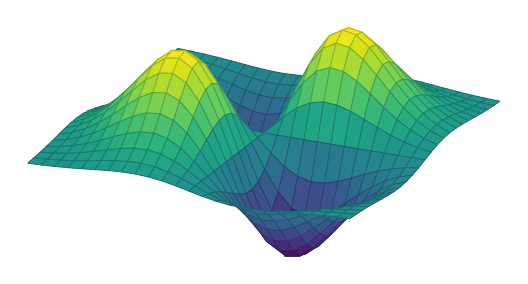
\begin{tikzpicture}[scale=0.875]
        \begin{axis}[hide axis,colormap/viridis]
            \addplot3[surf,domain=-2:2,y domain=-2:2] {7*x*y/exp(x^2+y^2)};
        \end{axis}
    \end{tikzpicture}
    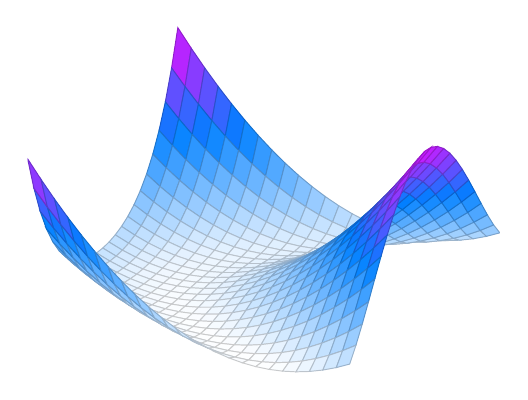
\begin{tikzpicture}[scale=0.875]
        \begin{axis}[hide axis,colormap/cool]
            \addplot3[surf,domain=-0.5:1.5,y domain=-1:1] {(1+y)^2+20*(x-y^2)^2};
        \end{axis}
    \end{tikzpicture}
}

\chapter{Optimization}
\label{ch:optimization}

\section{Linear Programming}

\begin{defn}
    In the context of an optimization problem:
    \begin{itemize}
        \item a \emph{constraint} is a condition that needs to be satisfied,
        \item the \emph{feasible region} $S \subseteq \R^n$ is the region that satisfies all constraints,
        \item and the \emph{objective function} is a function $f: S \to \R$ that is to be minimized or maximized.
    \end{itemize}
\end{defn}

\begin{figure}[ht!]
    \centering
    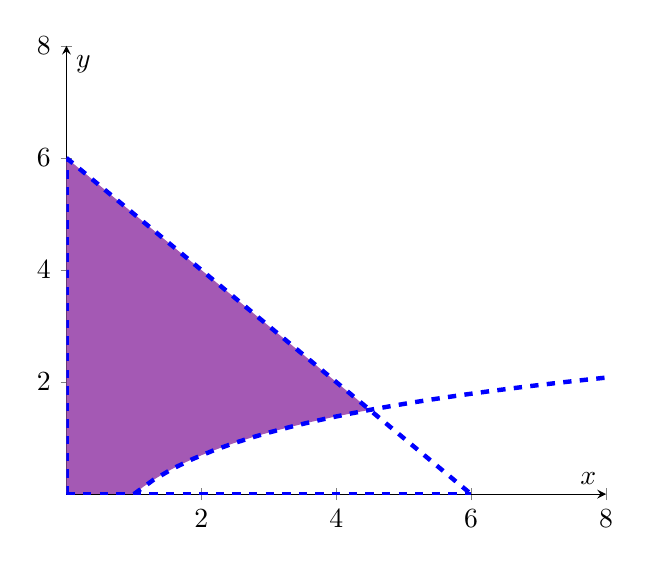
\begin{tikzpicture}[scale=1.0]
        \begin{axis}[
            axis x line=middle,
            axis y line=middle,
            ymin=0,ymax=8,ylabel=$y$,
            xmin=0,xmax=8,xlabel=$x$
        ]
            \begin{scope}
                \path[clip]
                    plot[domain=0:1] ({\x}, {0})
                    --plot[domain=1:4.49666] ({\x}, {ln(\x)})
                    --plot[domain=4.49666:0] ({\x}, {6-\x})
                    --plot[domain=0:6, variable=\y] ({0}, {\y})
                    --cycle;

                \fill [red!45!blue!65!] (0,0) rectangle (6,6);
            \end{scope}

            \plot[domain=0:6,blue,dashed,ultra thick] {6-\x};
            \plot[domain=1:8,blue,dashed,ultra thick] {ln(\x)};
            \plot[domain=0:6,blue,dashed,ultra thick] {0};
            \plot[domain=0:6,blue,dashed,ultra thick,variable=\y] ({0}, {\y});
        \end{axis}
    \end{tikzpicture}
\caption{Example feasible region (light purple) satisfying four constraints (dashed blue line)}
\label{fig:exmp-plant-feasible-region}
\end{figure}

\begin{exmp}
    Consider the problem of maximizing plant growth by manipulating quantities of two nutrients, $x_1$ and $x_2$. Let the plant height be $f(x_1, x_2) = 1 + x_1^2(x_2 - 1)^3e^{-x_1-x_2}$, with the constraints that $x_1 \geq 0$, $x_2 \geq 0$, $x_1 + x_2 \geq 6$, and $x_2 \geq \log x_1$. Then within the feasible region (depicted in Figure \ref{fig:exmp-plant-feasible-region}), $f$ is maximized by $(x_1, x_2) = (2, 4)$.
\end{exmp}

\begin{defn}
    For all $x \in \R^n$ and $\varepsilon > 0$, the \emph{$\varepsilon$-neighborhood} of $x$ is
    \[N_{\varepsilon}(x) = \left\{y \in \R^n \compbar \norm{x - y} < \varepsilon \right\}.\]
\end{defn}

\begin{exmp}
    In $\R^1$, $N_{3}(7)$ is $(4, 10)$.
\end{exmp}

\begin{defn}
    For any $S \subseteq \R^n$ and $x \in \R^n$, we say that $x$ is an \emph{interior point} of $S$ if there exists $N_{\varepsilon}(x) \subseteq S$. If every $N_{\varepsilon}(x)$ contains a point inside $S$ and a point not inside $S$, we say that $x$ is a \emph{boundary point} of $x$.
\end{defn}

\begin{defn}
    A set $S \subseteq \R^n$ is \emph{open} if every point in $S$ is an interior point of $S$, and \emph{closed} if $S$ contains every boundary point of $S$.
\end{defn}

\begin{exmp}
    In $\R^1$, any non-empty interval $[a, b]$ is closed, and non-empty $(a, b)$ is open.
\end{exmp}

\begin{exmp}
    Both $\emptyset$ and $\R^n \subseteq \R^n$ are both open and closed.
\end{exmp}

\begin{prop}
    Let $S \subseteq \R^n$. Then $S$ is open if and only if $\R^n - S$ is closed.
\end{prop}

\begin{proof}
    Assume that $S$ is open, and let $x$ be a boundary point of $\R^n - S$. Then for every $\varepsilon > 0$, by definition there exists $y, z \in N_{\varepsilon}(x)$ such that $y \in S$ and $z \in \R^n - S$. Therefore, $N_{\varepsilon}(x) \centernot\subseteq S$. It follows that $x \notin S$ by definition, and so $x \in \R^n - S$. Therefore, $\R^n - S$ contains every boundary point of itself, and so it is closed.

    Assume that $\R^n - S$ is closed, and let $x \in S$. Consider $N_{\varepsilon}(x)$. Since $\R^n - S$ contains all of its boundary points, $x$ cannot be a boundary point of $\R^n - S$, and so we know that there must be some $\varepsilon$ such that $N_{\varepsilon} \subseteq S$. Therefore, every $x \in S$ is an interior point of $S$, and so $S$ is closed by definition.
\end{proof}

\begin{exmp}
    We will examine a few cases in which minima and maxima may fail to first.

    \begin{itemize}
        \item Unbounded objective function, e.g. minimizing $\ln x$ such that $0 < x \leq 7$.
        \item Bounded objective function on open set, e.g. minimizing $\ln x$ such that $1 < x \leq 7$.
        \item Infeasible (feasible region is empty), e.g. minimizing $\ln x$ such that $1 < x$ and $x \leq 0.5$.
    \end{itemize}
\end{exmp}

\begin{exmp}
    When a solution exists, two distinct cases may occur.

    \begin{itemize}
        \item The solution is an interior point of the feasible region, e.g. minimizing $f(x) = 3 + (x - 2)^2$ such that $1 \leq x \leq 3$. The local minimum is $x^* = 2$, and $f'(x^*) = 0$.
        \item The solution is a boundary point of the feasible region, e.g. minimizing $f(x) = 3 + (x - 2)^2$ such that $x \leq 10$. Then $x^* = 10$, but $f'(x^*) \neq 0$.
    \end{itemize}
\end{exmp}

\begin{defn}
    Let $S \subseteq \R^n$ and $f: \R^n \to \R$. Consider $x^* \in S$. We say that $x^*$ is a \emph{global minimum} if for all $y \in S$, $f(x^*) \leq f(y)$, and a \emph{strict} global minimum if for all $y \in S - \{x^*\}$, $f(x^*) < f(y)$.
\end{defn}

\begin{defn}
    Let $S \subseteq \R^n$ and $f: \R^n \to \R$. Consider $x^* \in S$. We say that $x^*$ is a \emph{local minimum} if there exists an $\varepsilon$-neighborhood $N_{\varepsilon}(x^*)$ such that for all $y \in N_{\varepsilon}(x) \intersection S$, $f(x^*) \leq f(y)$, and a \emph{strict} local minimum if for all $y \in \left(N_{\varepsilon}(x) \intersection S\right) - \{x^*\}$, $f(x^*) < f(y)$.
\end{defn}

\begin{defn}
    Let $S \subseteq \R^n$ be a feasible region and $f: S \to \R$ an objective function. A \emph{stationary point} $x \in S$ is where $\nabla f(x) = \vec{0}.$
\end{defn}

\begin{rmk}
    Let $S \subseteq \R^n$, $x^*$ be an interior point of $S$, and $f: S \to \R$ be a sufficiently smooth continuous function. If $x^* \in S$ is a local minimum, then the \emph{gradient} of $f(x^*)$ is $\vec{0}$. However, $\nabla f(x^*) = \vec{0}$ does not imply that $x^*$ is a local minimum.
\end{rmk}

\subsection{Forms of Linear Programming Problems}

\begin{defn}
    A maximization or minimization linear programming problem in \emph{standard form} is a problem of the form:
    find $x \in \R^n$ that maximizes or minimizes $\transposeof{c}x$ such that $Ax = b$ and $x \geq \vec{0}$. The problem is said to be in \emph{canonical form} if the constraints are instead in the form $Ax \geq b$ (or $Ax \leq b$).
\end{defn}

\begin{exmp}
    Consider the problem of minimizing the cost per unit of chicken feed, while ensuring necessary nutrients are provided. Let $x_1, x_2, x_3, x_4$ denote the quantities of each of four ingredients, with cost per unit of $6.2$, $2.0$, $1.6$, and $3.2$ respectively. Let $n_1$, $n_2$, $n_3$ be the nutrients, with minimum required values of $6.2$, $11.9$, and $10.0$ respectively.

    \begin{minipage}{\linewidth}
        \begin{center}
        \captionof{table}{Nutrition values}
        \label{exmp-feed-nutrition-values}
        \begin{tabular}{c|cccc}
        & $x_1$ & $x_2$ & $x_3$ & $x_4$\\
        \hline
        $n_1$ & $1.2$ & $2.6$ & $0.0$ & $9.2$ \\ \hline
        $n_2$ & $3.9$ & $1.0$ & $0.8$ & $2.0$ \\ \hline
        $n_3$ & $6.0$ & $0.0$ & $4.0$ & $3.1$ \\
        \end{tabular}
        \end{center}
    \end{minipage}

    Let
    \[A = \begin{pmatrix}
        1.2 & 2.6 & 0.0 & 9.2 \\
        3.9 & 1.0 & 0.8 & 2.0 \\
        6.0 & 0.0 & 4.0 & 3.1
    \end{pmatrix},\; b = \begin{pmatrix}
        6.2 \\ 11.9 \\ 10.0
    \end{pmatrix},\; c = \begin{pmatrix}
        6.2 \\ 2.0 \\ 1.6 \\ 3.2
    \end{pmatrix},\; x = \begin{pmatrix}
        x_1 \\ x_2 \\ x_3 \\ x_4
    \end{pmatrix}\]
    then our problem is to minimize $\transposeof{c}x$ such that $Ax \geq b$ and $x \geq \vec{0}$. This form is the \emph{canonical form} of a linear programming problem.
\end{exmp}

\begin{rmk}
    We can easily convert problems expressed as a minimization problem into an equivalent maximization problem and vice versa, and between standard form and canonical form.
\end{rmk}

\begin{prop}
    Minimizing $\transposeof{c}x$ is equivalent to maximizing $-\transposeof{c}x$ (and so maximizing $\transposeof{c}x$ is equivalent to minimizing $-\transposeof{c}x$).
\end{prop}

\begin{proof}
    Let $P$ be a linear programming problem where we seek to minimize $\transposeof{c}x$, and let $S$ denote the feasible region of $P$. Now let $Q$ denote linear program where we seek to maximize $\transposeof{C}x$ that is otherwise identical to $P$. Let $x^{*}$ be a local minimum of $P$. By definition, there must exist some $\varepsilon$-neighborhood such that $\transposeof{c}x^{*} \leq \transposeof{c}y$ for all $y \in N_{\varepsilon}(x) \intersection S$. It follows that $-\transposeof{c}x^{*} \geq -\transposeof{c}y$ for all $y \in N_{\varepsilon}(x) \intersection S$, and so $x^{*}$ must be a local maximum of $Q$.
\end{proof}

\begin{prop}
    The constraint $Ax \geq b$ is equivalent to $-Ax \leq -b$, and $Ax \leq b$ is equivalent to $-Ax \geq -b$.
\end{prop}

\begin{prop}
    The constraint $Ax = b$ is equivalent to having both $Ax \geq b$ and $Ax \leq b$, and therefore is equivalent to $[A; -A] \geq [b; -b]$.
\end{prop}

\begin{prop}
    The constraint $Ax \geq b$ is equivalent to $Ax - z = b$, where $A \in M_{m \times n}(\R)$, $x \in \R^n$, and $z \in \R^m$ where $z \geq 0$. Here, $z$ is a vector of \emph{slack} variables.
\end{prop}

\begin{exmp}
    The constraints
    \begin{align*}
        a_{11}x_1 + a_{12}x_2 + a_{13}x_3 &\geq b_1 \\
        a_{21}x_1 + a_{22}x_2 + a_{23}x_3 &\geq b_2 \\
        a_{31}x_1 + a_{32}x_2 + a_{33}x_3 &\geq b_3 \\
        a_{41}x_1 + a_{42}x_2 + a_{43}x_3 &\geq b_4
    \end{align*}
    are equivalent to
    \begin{align*}
        a_{11}x_1 + a_{12}x_2 + a_{13}x_3 - x_4 &= b_1 \\
        a_{21}x_1 + a_{22}x_2 + a_{23}x_3 - x_5 &= b_2 \\
        a_{31}x_1 + a_{32}x_2 + a_{33}x_3 - x_6 &= b_3 \\
        a_{41}x_1 + a_{42}x_2 + a_{43}x_3 - x_7 &= b_4.
    \end{align*}
\end{exmp}

\begin{prop}
    We can incorporate the positivity constraints $x \geq 0$ into the general matrix constraints. The constraints $Ax \geq b$ and $x \geq 0$ are equivalent to \[\begin{bmatrix} A \\ I\end{bmatrix}x \geq \begin{bmatrix} b \\ 0 \end{bmatrix},\]
    and the constraints $Ax \leq b$ and $x \geq 0$ are equivalent to \[\begin{bmatrix} A \\ -I\end{bmatrix}x \leq \begin{bmatrix} b \\ 0 \end{bmatrix}.\]
\end{prop}

\begin{prop}
    We can transform an unconstrained problem into an equivalent problem with a positivity constraint.
\end{prop}

\begin{exmp}
    Consider the problem of minimizing $5x_1 + 6x_2$ such that $2x_1 - 3x_2 \geq 9$ and $x_1 + x_2 \geq -8$, with $x_1 \geq 0$ but $x_2$ unconstrained in sign. Define $x_2'$ and $x_2''$, and constrain $x_2', x_2'' \geq 0$. Let $x_2 = x_2' - x_2''$.
\end{exmp}

\begin{rmk}
    Constraints of the form $Ax = b$ are simply a system of equations, and therefore can be simplified using row operations by Theorem \ref{solutions-unchanged-by-row-ops}. Reduced row echelon form can help identified independent vs dependent variables.
\end{rmk}

\subsection{Polyhedrons}

\begin{defn}
    For non-zero $p \in \R^n$, the \emph{hyperplane} with normal vector $p$ is the orthogonal complement of $p$: \[\left\{x \in \R^n \compbar p \cdot x = 0 \right\},\]
    and the closed \emph{half-space} with normal vector $p$ is
    \[\left\{x \in \R^n \compbar p \cdot x \geq 0 \right\}.\]
    If we have $p \cdot x > 0$, we say it is an open half-space. We can replace $\geq$ and $>$ with $\leq$ and $<$ respectively.
\end{defn}

\begin{defn}
    A \emph{polyhedron} (or \emph{polyhedral set}) is the intersection of finitely many half spaces.
\end{defn}

\begin{defn}
    A polyhedron $P$ is \emph{bounded} if there exists $r \in \R$ such that $\norm{x} < r$ for all $x \in P$. A bounded polyhedron is known as a \emph{polytope}.
\end{defn}

\begin{prop}
    $P \subseteq \R^n$ is a polyhedron if and only if there exists $A \in M_{m \times n}(\R)$ and $b \in \R^m$ such that
    \[P = \left\{x \in \R^n \compbar Ax \geq b\right\}.\]
\end{prop}

\begin{defn}
    Let $X = \{x_1, \ldots, x_k\} \subset \R^n$. A \emph{convex combination} of $X$ is
    \[\lambda_1 x_1 + \lambda_2 x_2 + \cdots + \lambda_k x_k,\]
    where $\lambda_i \geq 0 \in \R$ and $\sum_{i=1}^{k}\lambda_i = 1$.
\end{defn}

\begin{defn}
    A set $S \subseteq \R^n$ is \emph{convex} if for any $x, y \in S$ and convex combination $z$ of $x$ and $y$, then $z \in S$.
\end{defn}

\begin{thm}
    Every polyhedron is convex.
\end{thm}

\begin{proof}
    Let $P = \left\{x \in \R^n, \compbar Ax \geq b\right\}$ be a polyhedron in $\R^n$. Let $x, y \in P$ and $z = \lambda x + (1 - \lambda) y$ be a convex combination of $x$ and $y$ for some $\lambda \in [0, 1]$.

    We know that $Ax \geq b$ and $Ay \geq b$, and want to show that $Az \geq b$. Since $z = \lambda x + (1 - \lambda)y$,
    \begin{align*}
        Az = A\left(\lambda x + (1 - \lambda)y\right) = \lambda Ax + (1 - \lambda)Ay \geq \lambda b + (1 - \lambda) b = b,
    \end{align*}
    and so $Az \geq b$.
\end{proof}

\begin{thm}
    A set $S \subseteq \R^n$ is convex if and only if every convex combination of every finite $X \subseteq S$ is in $S$.
\end{thm}

\begin{proof}
    We will prove this by showing that this is equivalent to the definition.

    $(\impliedby)$ If every convex combination of finite $X \subseteq S$ is in $S$, then every convex combination of $x, y \in S$ is in $X$.

    $(\implies)$ We will prove, via induction on $n = \abs{X}$, that if $z$ is a convex combination of $x, y \in S$ implies that $z \in S$, then every convex combination of $X \subseteq S$ is also in $S$.

    First, consider the base case of $n=1$, so $X = \{x\} \subseteq S$. The only convex combination of $X$ is simply $x$, and so every convex combination of $X$ is in $S$. Next, assume that if $z$ is a convex combination of $x, y \in S$ implies that $z \in S$, then every convex combination of $X \in S$ where $\abs{X} = n$ is also in $S$. For any $X' \subseteq S$ where $\abs{X'} = n+1$, there is some $X \subsetneq X'$ such that $\abs{X} = n$. Then every convex combination of $X$ is in $S$. Let \[\lambda_1x_1 + \cdots + \lambda_n x_n + \lambda_{n+1}x_{n+1}\] be a convex combination of $X$. Let $\Lambda = \lambda_1 + \cdots + \lambda_n$, and note that
    \[\alpha = \frac{\lambda_1}{\Lambda}x_1 + \cdots + \frac{\lambda_n}{\Lambda}x_n\] is a convex combination of $X$ and so must be in $S$ by by the induction hypothesis. Furthermore, note that
    \[\Lambda \alpha + \lambda_{n+1}x_{n+1}\] is our original convex combination of $X'$, but is also a convex combination of two points in $S$, and so is also in $S$ by assumption.
\end{proof}

\begin{defn}
    Let $S$ be a convex set, and consider $x \in S$. If $x$ being a convex combination of $y, z \in S$ implies that $x = y = z$, we say that $x$ is an \emph{extreme point}.
\end{defn}

\subsection{Basic Feasible Solutions}

\begin{defn}
    Let $c \in \R^n$, $A \in M_{m \times n}(\R)$, and $b \in \R^m$ be the linear program with feasibility region \[S = \left\{x \in \R^n \compbar Ax = b, x \geq \vec{0}\right\}.\] Let $A$ have rank $m$, or else eliminate redundant constraints until it does.

    Let $B$ be a subset of $m$ of the indices $\{1, \ldots, n\}$ such that the corresponding columns of $A$ form a basis for the column space of $A$ (which is $\R^m$ since $A$ has rank $m$). Let $A_B \in M_{m \times m}(\R)$ denote the invertible matrix of these columns.

    A \emph{basic feasible solution} is any $x \in S$ where $j \notin B$ implies $x_j = 0$.
\end{defn}

\begin{rmk}
    Without loss of generality, we can rearrange the columns of $A$ such that $A = [A_B | N]$, and then basic feasible solutions are precisely those $x \in S$ such that $x = \begin{bmatrix}
        x_B \\ x_N
    \end{bmatrix}$ where $x_N = \vec{0}$.
\end{rmk}

\begin{thm}
    Let $B \in M_{m \times m}(\R)$ have rank $m$, and $N \in M_{m \times (n-m)}(\R)$ where $m < n$, and then let $A = [B | N] \in M_{m \times n}(\R)$. Let $b \in \R^m$, so the feasible region is \[S = \left\{x \in \R^n \compbar Ax = b,\; x \geq \vec{0}\right\}.\]

    Then $x \in S$ is an extreme point of $S$ if and only if $x$ is a basic feasible solution of $S$.
\end{thm}

\begin{proof}\proofbreak
    ($\impliedby$) Suppose $x$ is a basic feasible solution of $S$, so $x = \begin{bmatrix}
        x_B \\ x_N
    \end{bmatrix}$ where $x_N = \vec{0}$. Let $x = \lambda x' + (1 - \lambda) x''$ be a non-trivial convex combination (so $0 < \lambda < 1$) of $x', x'' \in S$. We can represent $x'$ and $x''$ as $x' = \begin{bmatrix} x_B' \\ x_N' \end{bmatrix}$ and $x'' = \begin{bmatrix} x_B'' \\ x_N'' \end{bmatrix}$ respectively. Notice that we now have $x_N = \vec{0} = \lambda x_N' + (1 - \lambda)x_N''$. Since $x', x'' \in S$, we know $x_N', x_N'' \geq 0$ and so we necessarily have $x_N' = x_N'' = 0$. But then $x'$ and $x''$ are also basic feasible solutions. Since $A_{B}$ is invertible and $x, x', x'' \in S$, we know that $A_{B}x_B = A_{B}x_B'b = A_{B}x_B''$, and so $x = x' = x''$.

    ($\implies$) Suppose $x$ is not a basic feasible solution of $S$. Then $x = \begin{bmatrix}
        x_B \\ x_N
    \end{bmatrix}$ where $x_N$ is nonzero. We know that the columns of $A$ corresponding to the non-zero entries of $x$ must be linearly dependent, or else we can complete them to a basis for $\R^m$ and $x$ would be a basic feasible solution. Therefore, we know there exists non-zero $z$ such that $Az = \vec{0}$ and $z_i \neq 0$ implies $x_i \neq 0$. Note that for any $\alpha \in \R$, $A(x + \alpha z) = Ax + \alpha Az = b$, so any $x + \alpha z \geq \vec{0}$ is a feasible solution. Since $x_i$ is strictly greater than zero when $z_i \neq 0$, for sufficiently small $\varepsilon$ the points $x + \varepsilon z$ and $x - \varepsilon z$ must be feasible. Then $x = \frac{1}{2}\left(x + \varepsilon z\right) + \left(1 - \frac{1}{2}\right)\left(x - \varepsilon z\right)$, and so $x$ can be expressed as a non-trivial convex combination in $S$ and therefore is not extreme.
\end{proof}

\subsection{Simplex Method}

\begin{defn}
    Consider a linear program in standard form. Given a choice of basis $B$ such that $A = [B | N]$, the \emph{pre-tableau} is the matrix
    \begin{align*}
        \left[\begin{array}{c|c|c|c}
            1 & -\transposeof{c_B} & -\transposeof{c_N} & 0 \\
            \hline
            \vec{0} & B & N & b
        \end{array}\right].
    \end{align*}
    In other words, we have augment $A = [B|N]$ with the constraint values $b$, and then again with a new variable $z$ in the first column/row such that $z - \transposeof{c}x = 0$. Note that $z$ is therefore the value of the objective function.
\end{defn}

\begin{defn}
    Given a linear program in standard form, and basic feasible solution $\transposeof{x} = [\transposeof{x_B}, \vec{0}]$, the corresponding \emph{basic feasible simplex tableau} is the matrix
    \begin{align*}
        \left[\begin{array}{c|c|c|c}
            1 & 0 & \transposeof{c_B}B^{-1}N-\transposeof{c_N} & \transposeof{c_B}B^{-1}b \\
            \hline
            \vec{0} & I & B^{-1}N & B^{-1}b
        \end{array}\right].
    \end{align*}
\end{defn}

\begin{rmk}
    The basic feasible tableau is the reduced row echelon form of the pre-tableau. It can also be obtain by left-multiplying the pre-tableau by
    \begin{align*}
        \left[\begin{array}{c|c}
            1 & \transposeof{c_B}B^{-1} \\
            \hline
            \transposeof{\vec{0}} & B^{-1}
        \end{array}\right].
    \end{align*}
\end{rmk}

\begin{rmk}
    We can see that $z + (\transposeof{c_B}B^{-1}N-\transposeof{c_N})x_N = \transposeof{c_B}B^{-1}b$, so $z = \transposeof{c_B}B^{-1}b + (\transposeof{c_N} - \transposeof{c_B}B^{-1}N)x_N$. We often denote this as
    \[z = \transposeof{c_B}B^{-1}b + \transposeof{r_N}x_N,\]
    where
    \[\transposeof{r_N} = \transposeof{c_N} - \transposeof{c_B}B^{-1}N.\]
\end{rmk}

In the simplex, we start with a linear program $A, b, c$ in standard form. Assuming we already know a basis that leads to a basic feasible solution, we form the pre-tableau and either row-reduce or multiply through by the matrix from the above remark to obtain the basis feasible tableau.

To illustrate the linear program, we will consider
\begin{align*}
    A =
    \begin{bmatrix}
        2 & -1 & 3 & 7 & 1 & 2 & 8 \\
        5 & 2 & -8 & -1 & 2 & 0 & 1 \\
        4 & 6 & -2 & 4 & 1 & 3 & -5
    \end{bmatrix},\;\;
    b = \begin{bmatrix}
        2 \\ 4 \\ 3
    \end{bmatrix},\;\;
    \transposeof{c} = [6, -3, 2, 1, -1, 7, 1].
\end{align*}

We will use columns $1$, $3$, and $7$ as our basis columns, however we will leave the columns in their original order to make bookkeeping easier. Our pre-tableau is
\begin{align*}
    \left[\begin{array}{c|ccccccc|c}
        1 & -6 & 3 & -2 & -1 & 1 & -7 & -1 & 0 \\
        \hline
        0 & 2 & -1 & 3 & 7 & 1 & 2 & 8 & 2 \\
        0 & 5 & 2 & -8 & -1 & 2 & 0 & 1 & 4 \\
        0 & 4 & 6 & -2 & 4 & 1 & 3 & -5 & 3
    \end{array}\right].
\end{align*}

Row-reducing to the reduced row echelon form (while treating columns $1$, $3$, and $7$ as leading columns) brings us to our first basic feasible tableau:
\begin{align*}
    \left[\begin{array}{c|ccccccc|c}
        1 & 0 & 9.35 & 0 & 11.06 & 2.82 & -1.22 & 0 & 4.93 \\
        \hline
        0 & 1 & 1.03 & 0 & 1.62 & 0.31 & 0.82 & 0 & 0.81 \\
        0 & 0 & 0.33 & 1 & 1.14 & -0.05 & 0.50 & 0 & 0.01 \\
        0 & 0 & -0.51 & 0 & 0.04 & 0.07 & -0.14 & 1 & 0.04
    \end{array}\right].
\end{align*}

Now, we \emph{pivot} to a new (and improved!) basic feasible tableau by choosing a non-basis column to turn into a basis column. We make the greediest choice by choose the $4$th column ($5$th of the overall tableau) since it has the largest improvement to our objective function per unit change in the corresponding non-basis variable.

Letting $j = 4$, we choose the $k$th row (excluding the objective row on top) by \[\argmin_{k}\frac{b_k}{A_{kj}} \mathrm{ where } A_{kj} > 0.\] This gives us the $2$nd row, so we row-reduce again, replace the column whose leading term choose in the $2$nd row (which is column $3$) with column $4$. To do this, we treat column $4$ as if it was the second column while row-reducing. Our new basis columns are $1$, $4$, and $7$, giving us our second basic feasible tableau:
\begin{align*}
    \left[\begin{array}{c|ccccccc|c}
        1 & 0 & 6.14  & -9.67 & 0 & 3.29  & -6.01 & 0 & 4.81 \\
        \hline
        0 & 1 & 0.56  & -1.41 & 0 & 0.37  & 0.11  & 0 & 0.79 \\
        0 & 0 & 0.28  & 0.87  & 1 & -0.04 & 0.43  & 0 & 0.01 \\
        0 & 0 & -0.57 & -0.03 & 0 & 0.06  & -0.15 & 1 & 0.04
    \end{array}\right].
\end{align*}

Note that the objective function value has decreased from $4.93$ to $4.81$. We now continue pivoting in the manner, the objective function value decreasing from $4.81$, to $4.6$, to $-2.45$, to $-2.46$. When there are no positive entries in the objective function row (top row), there are no more improvements that can be made by changing our choice of basis and we have reached optimality.

\subsection{Two-Phase Method}

The Two-Phase Method is a technique for coming up with the initial basic feasible solution need to start off the Simplex Method. In Phase I, we solve a different linear program to find the initial basic feasible solution, and then in Phase II we use that basic feasible solution to apply the simplex method to the original linear program. We take a problem in standard form with constraints $Ax = b$, $x \geq 0$ where $A \in M_{m \times n}(\R)$. We then introduce \emph{artificial variables} $x_{n+1}, x_{n+2}, \ldots, x_{n+m}$ for each constraint (row) in $A$. Let $x'$ denote the vector obtained by appending the artificial variables to $x$.

For Phase I, we solve a different problem using the Simplex Method: minimizing $x_{n+1} + x_{n+2} + \cdots + x_{n+m}$ such that $[A|I]x' = b$, $x' \geq 0$. Notice that any feasible solution to this new problem is a feasible solution to the original linear program if the objective function value is zero. Therefore, the $x$ part of an optimal solution $x'$ to the new problem is a feasible solution to the original if $x'$ has objective function value zero. If the optimal solution $x'$ has a positive objective function value, then no feasible solution exists for the original linear program.

Note that
\begin{align*}
    x' = \begin{bmatrix}
        x \\
        x_{n+1} \\
        \vdots \\
        v_{n+m}
    \end{bmatrix} = \begin{bmatrix}
        0 \\
        b_1 \\
        \vdots \\
        b_m
    \end{bmatrix}
\end{align*}
is always a basic feasible solution to the Phase I problem. Therefore, we can immediately apply the Simplex method to determine the feasibility of the original linear program, and find a feasible solution if one exists. Additionally, since the number of columns in a basis for either linear program is the same (always just $m$), the feasible solution given to us by Phase I must in fact be a basic feasible solution for Phase II.

\subsection{Big-M Method}

In the Big-M method, we essentially combine the two phases of the Two-Phase method by using the objective function
\begin{align*}
    \transposeof{c}x + M(x_{n+1} + x_{n+2} + \cdots + x_{n+m}),
\end{align*}
where $M$ is a very large value. This penalizes the artificial variables and causes them to be zero in any optimal solution. Setting the artificial variables to $b$ gives us an initial basic feasible solution. If a basic feasible solution exists where the artificial variables are zero, the first $m$ pivots will replace each artificial variable with non-artificial variables, and so the final optimal solution will be a solution to the original linear program.

\subsection{Duality}

\begin{defn}{Canonical or symmetric duality}\proofbreak
    Consider a linear program of the form minimize $\transposeof{c}x$ such that $Ax \geq b$ and $x \geq \vec{0}$. The \emph{dual} problem is maximizing $\transposeof{b}y$ such that $\transposeof{A}y \leq c$ and $y \geq \vec{0}$. The original linear program is referred to as the \emph{primal} probem in relation to its dual.
\end{defn}

\begin{exmp}
    Consider minimizing $1x_1 + 2x_2$ such that
    \begin{align*}
        3x_1 + 4x_2 &\geq 9, \\
        5x_1 + 6x_2 &\geq 10, \\
        7x_1 + 8x_2 &\geq 11, \\
        x_1, x_2 &\geq 0.
    \end{align*}

    The dual problem is maximizing $9y_1 + 10y_2 + 11y_3$ such that
    \begin{align*}
        3y_1 + 5y_2 + 7y_3  &\leq 1, \\
        4y_1 + 6y_2 + 8y_3  &\leq 2, \\
        y_1, y_2, y_3 &\geq 0.
    \end{align*}
\end{exmp}

\begin{defn}{Standard duality}\proofbreak
    Consider a linear program of the form minimization of $\transposeof{c}x$ such that $Ax = b$ and $x \geq \vec{0}$. The \emph{dual} problem is maximizing $\transposeof{b}y$ such that $\transposeof{A}y \leq c$, \emph{without} a non-negativity constraint on $y$. The original linear program is again referred to as the \emph{primal} probem in relation to its dual.
\end{defn}

\begin{rmk}
    We can derive the canonical form of duality from the standard form, and vice versa. Imagine we know that the dual of minimizing $\transposeof{c}x$ such that $Ax = b$ and $x \geq \vec{0}$ was to maximize $\transposeof{b}y$ such that $\transposeof{A}y \leq c$. If we were now given a linear program in canonical form and wanted to find its dual, we could first convert it into standard form by the introduction of slack variables, obtaining minimize $\transposeof{c}x$ such that $[A|-I]\begin{bmatrix}x \\ z\end{bmatrix} = b$ such that $\begin{bmatrix}x \\ z\end{bmatrix} \geq 0$. The standard dual of this is to maximize $\transposeof{b}y$ such that $\transposeof{[A|-I]}y \leq \begin{bmatrix}c \\ \vec{0}\end{bmatrix}$, which is equivalent to maximizing $\transposeof{b}y$ such that $\transposeof{A}y \leq c$ and $y \geq \vec{0}$ (from $-y \leq \vec{0}$).
\end{rmk}

\begin{prop}
    The canonical and standard duals of equivalent linear programs are equivalent.
\end{prop}

\begin{proof}
    See figure \ref{fig:duality-equivalence}.
\end{proof}

\begin{figure}[ht]
    \centering
    \begin{tikzpicture}[{baseline=(current bounding box.north)}]
        \node[align=center] at (-3,2.5) {$
            \begin{aligned}
                \mathrm{min.}\;\transposeof{c}&x \\
                \mathrm{s.t.}\;A&x \geq b, \\
                        &x \geq \vec{0}.
            \end{aligned}
        $};
        \node[align=center] at (3,2.5) {$
            \begin{aligned}
                \mathrm{max.}\;\transposeof{b}&y \\
                \mathrm{s.t.}\;\transposeof{A}&y \leq c, \\
                        &y \geq \vec{0}.
            \end{aligned}
        $};
        \node[align=center] at (-3,-3) {$
            \begin{aligned}
                \mathrm{min.}\;\transposeof{\begin{bmatrix}c \\ \vec{0}\end{bmatrix}}&\begin{bmatrix}x \\ z\end{bmatrix} \\
                \mathrm{s.t.}\;\left[A|-I\right]&\begin{bmatrix}x \\ z\end{bmatrix} = b, \\
                        &x, z \geq \vec{0}.
            \end{aligned}
        $};
        \node[align=center] at (3,-3) {$
            \begin{aligned}
                \mathrm{max.}\;&\transposeof{b}y \\
                \mathrm{s.t.}\;&\begin{bmatrix}\transposeof{A} \\ -I\end{bmatrix}y \leq \begin{bmatrix}c \\ \vec{0}\end{bmatrix}.
            \end{aligned}
        $};

        \draw[ultra thick, blue, ->] (-1, 3) -- (1, 3);
        \draw[ultra thick, red, ->] (-1, -3) -- (1, -3);
        \draw[ultra thick, black, <->] (3, -1) -- (3, 1);
        \draw[ultra thick, black, <->] (-3, 1) -- (-3, -1);

    \end{tikzpicture}
\caption{Equivalence of dualities}
\label{fig:duality-equivalence}
\end{figure}

\newpage

\begin{prop}
    Given a primal linear program, the dual of the dual is the primal.
\end{prop}

\begin{proof}
    Consider a linear program in canonical form.  By definition, the dual is maximizing $\transposeof{b}y$ such that $\transposeof{A}y \leq c$ and $y \geq 0$. This program is equivalent to minimizing $-\transposeof{b}y$ such that $-\transposeof{A}y \geq -c$ and $y \geq 0$. The dual of this equivalent form of the dual is to maximizing $-\transposeof{c}x$ such that $\transposeof{\left(-\transposeof{A}\right)}x \leq -b$ and $x \geq 0$. Finally, this program is equivalent to minimizing $\transposeof{c}x$ such that $Ax \geq b$ and $x \geq 0$, which is the primal linear program.
\end{proof}

\begin{thm}{Weak Duality}\label{weak-duality}\proofbreak
    Consider a linear program and its dual, and $x, y$ feasible solutions to the primal and dual programs respectively. Then the objective function value at $y$ in the dual is less than or equal to the objective function value at $x$ in the primal.
\end{thm}

\begin{proof}
    When the primal is in standard form, we have $Ax = b$, $x \geq \vec{0}$ and $\transposeof{A}y \leq c$. It follows that $\transposeof{b}y = \transposeof{(Ax)}y = \transposeof{x}\transposeof{A}y$. Since we have $x \geq \vec{0}$, we know that $\transposeof{x}\transposeof{A}y \leq \transposeof{x}c$, and so $\transposeof{b}y \leq \transposeof{c}x$.

    When the primal is in canonical form, we have $Ax \geq b$, $x \geq \vec{0}$, $\transposeof{A}y \leq c$, and $y \geq 0$. Since $y \geq \vec{0}$, $Ax \geq b$ implies that $\transposeof{b}y \leq \transposeof{(Ax)}y$, and so $\transposeof{b}y \leq \transposeof{x}\transposeof{A}y$. Furthermore, since $\transposeof{A}y \leq c$ and $x \geq \vec{0}$, $\transposeof{x}\transposeof{A}y \leq \transposeof{x}c = \transposeof{c}x$. Combining these, we arrive at $\transposeof{b}y \leq \transposeof{c}y$.
\end{proof}

\begin{cor}
    The optimal objective value function in the dual is less than or equal to the optimal objective function value in the primal.
\end{cor}

\begin{cor}{Supervisor principle}\label{supervisor-principle}\proofbreak
    If $\transposeof{b}y = \transposeof{c}x$, then $x$ and $y$ are optimal in their respective linear programs.
\end{cor}

\begin{thm}{Strong Duality}\label{strong-duality}\proofbreak
    Suppose a linear program has a feasible solution and its objective function is bounded from below. Then the linear program and its dual have optimal solutions $x$ and $y$ respectively, and the objective function value of $x$ and $y$ are equal.
\end{thm}

\begin{proof}
    Consider the primal in standard form. We can apply the Simplex method or similar to obtain an optimal basic feasible solution $x^*$. Without loss of generality, we can assume that the final basis consists of the first $m$ columns of $A$.

    By the terminating condition of the Simplex method, we know that
    \begin{align*}
        \transposeof{r_N} = \transposeof{c_N} - \transposeof{c_B}B^{-1}N \geq \vec{0}.
    \end{align*}
    Let
    \begin{align*}
        \transposeof{y^*} = \transposeof{c_B}B^{-1}.
    \end{align*}

    Since $\transposeof{r_N} \geq \vec{0}$, we know that
    \begin{align*}
        \transposeof{c_B}B^{-1}N \leq \transposeof{c_N},
    \end{align*}
    and so it follows that
    \begin{align*}
        \transposeof{y^*}A = \transposeof{c_B}B^{-1}[B|N] = [\transposeof{c_B}|\transposeof{c_B}B^{-1}N] \leq [\transposeof{c_B}|\transposeof{c_N}] = \transposeof{c},
    \end{align*}
    so $y^*$ is a feasible solution to the dual. Now we can show that the objective function values are equal:
    \begin{align*}
        \transposeof{y^*}b = \transposeof{c_B}B^{-1}b = \transposeof{\begin{bmatrix}c_B \\ \vec{0}\end{bmatrix}}\begin{bmatrix}x_B \\ \vec{0}\end{bmatrix} = \transposeof{c}x^*.
    \end{align*}

    Therefore, $y^*$ is an optimal solution to the dual linear program by the supervisor principle \ref{supervisor-principle}.
\end{proof}

\begin{defn}
    A basic feasible solution $b$ to a linear program with basis $B$ is \emph{non-degenerate} when $B^{-1}b > \vec{0}$.
\end{defn}

Consider solving a linear program $A, b, c$ in standard form by the Simplex method. What happens if we replace $b$ with $b' = b + \Delta b$ for some arbitrary $\Delta b$? If we replaced $B^{-1}b$ with $B^{-1}(b + \Delta b)$ and $\transposeof{c_B}B^{-1}b$ with $\transposeof{c_B}B^{-1}(b + \Delta b)$ in just the final basic feasible simplex tableau, what happens?

If $B^{-1}(b + \Delta b) \geq \vec{0}$, then we still have a basic feasible solution! Furthermore, since the objective row would still be non-positive, our solution would also be an \emph{optimal} basic feasible solution. This would very likely only occur when $\Delta b$ is fairly small.

If the linear program is non-degenerate, there always exists such $\Delta b$ small enough.

In the corresponding dual linear program, we know that
\begin{align*}
    \transposeof{y^*} = \transposeof{c_B}B^{-1}.
\end{align*}
We also have $\transposeof{c}x^* = \transposeof{y^*}b$, and so when we replace $b$ with $b'$ we get
$\transposeof{c}{x'}^{*} = \transposeof{y^*}(b + \Delta b) = \transposeof{y^*}b + \transposeof{y^*}\Delta b$. Therefore,
\begin{align*}
    \frac{\partial\transposeof{c}{x}^{*}}{\partial b_i} = y_i^*.
\end{align*}

\begin{defn}
    Vectors $x, y \in \R^n$ are \emph{complementary} if $x_i \neq 0 \implies y_i = 0$ and $y_i \neq 0 \implies x_i = 0$.
\end{defn}

\begin{prop}\label{complementary-orthogonal}
    If $x \geq 0$ and $y \geq 0$, then $x$ and $y$ are complementary if and only if $\transposeof{x}y = 0$.
\end{prop}

\begin{proof}
    If $x$ and $y$ are complementary, then $x_iy_i = 0$, and so $\transposeof{x}y = 0$.

    Since $x \geq 0$ and $y \geq 0$, we know $x_iy_i \geq 0$. If $\transposeof{x}y = 0$, then we must have $x_iy_i = 0$. Therefore at least one of $x_i$ and $y_i$ is zero and so $x$ and $y$ are complementary.
\end{proof}

\begin{thm}{Complementary slackness}\label{complementary-slackness}\proofbreak
    Consider a linear program $A, b, c$ in standard form. Let $x \in \R^n$ be a feasible solution. Let $y \in \R^m$ be a feasible solution in the dual. Then $x$ and $y$ are optimal solutions if and only if $c - \transposeof{A}y$ is complentary to $x$.
\end{thm}

\begin{proof}
    Recall that
    \begin{align*}
        \transposeof{b}y = \transposeof{(Ax)}y = \transposeof{x}\transposeof{A}y \leq \transposeof{x}c = \transposeof{c}x.
    \end{align*}
    By the supervisor principle \ref{supervisor-principle}, $x$ and $y$ are optimal if and only if $\transposeof{b}y = \transposeof{c}x$, which is equivalent to $\transposeof{x}\transposeof{A}y = \transposeof{x}c$. Therefore,
    \begin{align*}
        \transposeof{x}\left(c - \transposeof{A}y\right) = \vec{0}.
    \end{align*}

    Since $y$ is feasible in the dual, by definition $\transposeof{A}y \leq c$, and so $c - \transposeof{A}y \geq \vec{0}$. Furthermore, $x \geq 0$ and so by Proposition \ref{complementary-orthogonal} it follows that this occurs precisely when $x$ and $c - \transposeof{A}y$ are complementary.
\end{proof}

\subsection{Dual Simplex Method}

In the dual simplex method, we have a linear program in standard form. Unlike when we start the simplex method, rather than knowing a starting feasible solution and working towards optimality, we know a starting solution that is essentially optimal and works towards feasibility. We actually start with a vector $y$ that is feasible in the dual linear program, and work towards making the corresponding primal vector $x$ feasible in the primal. Due to the setup of the dual simplex method, both $y$ and $x$ will have the same objective function value, and so once $x$ is feasible we have an optimal solution by the supervisor principle \ref{supervisor-principle}.

\begin{defn}{Basic tableau}\proofbreak
    A basic tableau is a tableau formed from a basic, but not necessarily feasible, solution.
\end{defn}

Given a linear program in standard form and corresponding basic tableau, we have $\transposeof{y} = \transposeof{c_B}B^{-1}$ and $x = B^{-1}b$. Recall that $y$ is an optimal solution to the dual problem when:
\begin{itemize}
    \item $Ax = b$,
    \item $x \geq 0$,
    \item $\transposeof{A}y \leq c$,
    \item $\transposeof{c}x = \transposeof{b}y$.
\end{itemize}

The first condition, that $Ax = b$ is necessarily satisfied by any basic tableau. The fourth, that $\transposeof{c}x = \transposeof{b}y$, is also satisfied since $\transposeof{c_B}B^{-1}b = \transposeof{y}b = \transposeof{b}y$ and $\transposeof{c_B}B^{-1}b = \transposeof{c}x$. The third condition, that $\transposeof{A}y \leq c$, is satisfied when $r \geq 0$. Since the top row of the tableau is $-r$, to have dual feasibility at the start of the dual simplex method we require that $-r \leq 0$ --- that is, that the top row of the basic tableau is non-positive other than the constant $1$. Therefore, we need to come up with a ``dual pivot'' that preserves these properties while working towards achieving the second condition.

To dual pivot, we choose the row $j$ with the most-negative value in $B^{-1}b$, and pick a column to row-reduce on. Since we need to maintain a non-positive top row $-r$, we want to pick the column $k$ by \[\argmin_{k}\frac{r_k}{A_{jk}} \mathrm{ where } A_{jk} < 0.\]

\section{Nonlinear}

\subsection{Convex and Lipschitz smooth functions}

\begin{defn}
    A set $S \subseteq \R^n$ is said to be \emph{convex} if $x, y \in S$ implies $tx + (1-t)y \in S$ for all $t \in [0, 1]$.
\end{defn}

\begin{lemma}\label{lemma:convex-sets}
    Let $A, B, C \subseteq \R^n$ be convex sets. The following are also convex:
    \begin{itemize}
        \item $\R^{+}A = \left\{\lambda x : \lambda \geq 0, x \in A\right\}$,
        \item $A + B = \left\{x + y : x \in A, y \in B\right\}$,
        \item $A \intersect B$,
        \item $T(A)$ and $T^{-1}(A)$, where $T: \R^n \to \R^n$ is a linear map (even if $T$ is not invertible).
    \end{itemize}
\end{lemma}

\begin{proof}\proofbreak
    \begin{itemize}
        \item If $x, y \in \R^{+}A$, then $x = \lambda_1s_1, y = \lambda_2s_2$ for some $\lambda_1, \lambda_2 \in \R^+$ and $s_1, s_2 \in A$. Therefore,
        \begin{align*}
            tx + (1-t)y &= t\lambda_1s_1 + (1 - t)\lambda_2s_2 = \lambda_3\left[us_1 + (1-u)s_2\right],
        \end{align*}
        where
        \begin{align*}
            \lambda_3 &= t\lambda_1 + (1-t)\lambda_2 \\
            u &= \frac{t\lambda_1}{\lambda_3}.
        \end{align*}
        Since $\lambda_1, \lambda_2 \geq 0$, it follows that $u \in [0, 1]$ and so $us_1 + (1-u)s_2 = s_3 \in A$. Furthermore, $\lambda_3$ is strictly positive, so $tx + (1-t)y = \lambda_3s_3 \in \R^{+}A$.
        \item If $x = a_1 + b_1$ and $y = a_2 + b_2$, then $tx + (1-t)y = (ta_1 + (1-t)a_2) + (tb_1 + (1-t)b_2) \in A + B$.
        \item If $x \in A \intersect B$ and $y \in A \intersect B$, then of course $tx + (1-t)y \in A$ and $tx + (1-t)y \in B$ by convexity of $A$ and $B$, so $tx + (1-t)y \in A \intersect B$.
        \item Follows immediately from linearity of $T$ and the fact convex combinations are linear combinations.
    \end{itemize}
\end{proof}

\begin{defn}
    Let $S \subseteq \R^n$ be a non-empty convex set, and let $f: S \to \R$. We say that $f$ is \emph{convex} when
    \begin{align*}
        f\left(\lambda x + (1 - \lambda)y\right) \leq \lambda f(x) + (1 - \lambda)f(y)
    \end{align*}
    for all $x, y \in S$ and $\lambda \in [0, 1]$.

    Similarly, we say that $f$ is \emph{strictly convex} when
    \begin{align*}
        f\left(\lambda x + (1 - \lambda)y\right) < \lambda f(x) + (1 - \lambda)f(y)
    \end{align*}
    for all $x, y \in S$ and $\lambda \in (0, 1)$.

    We analogously define \emph{concave} and \emph{strictly concave} functions using $\geq$ and $>$ respectively.
\end{defn}

\begin{rmk}
    Note that we use an open interval for $\lambda$ in the strict case, and a closed interval otherwise. This is because at $\lambda = 0$ or $\lambda = 1$ we will always have equality.
\end{rmk}

\begin{defn}
    Let $S \subseteq \R^n$, and consider $f: S \to \R$. The \emph{epigraph} of $f$
    \begin{align*}
        \left\{\begin{pmatrix}
            x \\ y
        \end{pmatrix} \in S \times \R : y \geq f(x)\right\} \subseteq \R^{n+1}
    \end{align*}
    and is denoted by $\epigraphof{f}$. That is, the epigraph is the set of all points above the graph of the function.
\end{defn}

\begin{prop}\label{epigraph-convexity}
    Let $S \subseteq \R^n$, and consider $f: S \to \R$. Then $f$ is a convex function if and only if $\epigraphof{f}$ is a convex set.
\end{prop}

\begin{proof}\proofbreak
    ($\implies$) Assume that $f$ is convex. Then for any $\transposeof{[x_1, y_1]}, \transposeof{[x_2, y_2]} \in \epigraphof{f}$ and $\lambda \in [0, 1]$, we know that
    \begin{align*}
        f(\lambda x_1 + (1 - \lambda)x_2) \leq \lambda f(x_1) + (1 - \lambda)f(x_2) \leq \lambda y_1 + (1 - \lambda)y_2.
    \end{align*}
    Therefore,
    \begin{align*}
        \lambda \begin{bmatrix}
            x_1 \\ y_1
        \end{bmatrix} + (1-\lambda)\begin{bmatrix}
            x_2 \\ y_2
        \end{bmatrix} = \begin{bmatrix}
            \lambda x_1 + (1 - \lambda)x_2 \\
            \lambda y_1 + (1 - \lambda)y_2
        \end{bmatrix} \in \epigraphof{f},
    \end{align*}
    and so $\epigraphof{f}$ is a convex set.

    ($\impliedby$) Assume that $\epigraphof{f}$ is a convex set. Since we trivially have $f(x) \leq f(x)$ for all $x \in S$, we know that for any $x_1, x_2 \in S$ we have
    \begin{align*}
        \transposeof{[x_1, f(x_1)]}, \transposeof{[x_2, f(x_2)]} \in \epigraphof{f}.
    \end{align*}
    Since $\epigraphof{f}$ is convex, for all $\lambda \in [0, 1]$ we also know that
    \begin{align*}
        \lambda \begin{bmatrix}
            x_1 \\ f(x_1)
        \end{bmatrix} + (1-\lambda)\begin{bmatrix}
            x_2 \\ f(x_2)
        \end{bmatrix} = \begin{bmatrix}
            \lambda x_1 + (1 - \lambda)x_2 \\
            \lambda f(x_1) + (1 - \lambda)f(x_2)
        \end{bmatrix} \in \epigraphof{f}.
    \end{align*}
    Therefore,
    \begin{align*}
        f(\lambda x_1 + (1 - \lambda)x_2) \leq \lambda f(x_1) + (1-\lambda)f(x_2)
    \end{align*}
    by the definition of $\epigraphof{f}$, and so $f$ is a convex function.
\end{proof}

\begin{thm}{Support Theorem}\label{support-theorem}\proofbreak
    Let $S \subseteq \R^n$ be a convex set, and let $\bar{x}$ be a boundary point of $S$. There exists a hyperplane containing $\bar{x}$ such that $S$ is contained in an associated closed half-space.
\end{thm}

\begin{thm}\label{convex-function-tangent-hyperplane}
    Let $S \subseteq \R^n$ be an open convex set, and let $f: S \to \R$ be continuously differentiable. Then the following are equivalent:
    \begin{itemize}
        \item $f$ is a convex function,
        \item $f(x) \geq f(\bar{x}) + \langle \nabla f(\bar{x}), x - \bar{x}\rangle$ for all $x, \bar{x} \in S$,
        \item $\langle \nabla f(x) - \nabla f(y), x - y \rangle \geq 0$.
    \end{itemize}
\end{thm}

\begin{proof}
    Suppose that (1) holds, so $f(\bar{x} + t(x - \bar{x})) \leq tf(\bar{x}) + (1 - t)f(x)$ by definition of a convex function. Therefore,
    \begin{align*}
        \frac{f(\bar{x} + t(x - \bar{x})) - f(\bar{x})}{t} \leq f(x) - f(\bar{x}).
    \end{align*}
    Taking the limit as $t \to 0$, we obtain (2): $\langle \nabla f(\bar{x}), x - \bar{x} \rangle \leq f(x) - f(\bar{x})$.

    Now instead let $x, y \in \R^n$ and define $z_t = ty + (1-t)x$. Suppose that (2) holds, so for all $t \in [0, 1]$ we have
    \begin{align*}
        f(x) \geq f(z_t) + \langle \nabla f(z_t), x - z_t\rangle, \\
        f(y) \geq f(z_t) + \langle \nabla f(z_t), y - z_t\rangle.
    \end{align*}
    Since $t \geq 0$ and $1-t \geq 0$, it follows that we may take a convex combination of the inequalities in order to obtain
    \begin{align*}
        (1-t)f(x) + tf(y) \geq \langle \nabla f(z_t), (1-t)x + ty \rangle,
    \end{align*}
    and so $f$ is a convex function. Therefore, condition (1) holds if and only if (2) holds.

    Suppose that (2) holds, so
    \begin{align*}
        f(x) \geq f(y) + \langle \nabla f(y), x - y\rangle, \\
        f(y) \geq f(x) + \langle \nabla f(x), y - x\rangle.
    \end{align*}
    Adding these inequalities, we obtain
    \begin{align*}
        f(x) + f(y) \geq f(x) + f(y) + \langle \nabla f(y) - \nabla f(x), x - y \rangle,
    \end{align*}
    and so (3) holds: $\langle \nabla f(x) - \nabla f(y), x - y \rangle \geq 0$.

    Finally, suppose (3) holds, and we will show (2) holds. Define $\varphi(t) = f(x + t(y - x))$. Then by applying the Fundamental Theorem of Calculus we obtain
    \begin{align*}
        \varphi(1) &= \varphi(0) + \int_{0}^{1}\varphi'(t)dt \\
        \varphi(1) &= \varphi(0) + \varphi'(0) - \int_{0}^{1} \varphi'(0)dt + \int_{0}^{1}\varphi'(t)dt \\
    \end{align*}
    Therefore,
    \begin{align*}
        f(y) &= f(x) + \langle \nabla f(x), y - x \rangle - \int_{0}^{1}\left(\langle \nabla \varphi(0), y - x \rangle - \langle \nabla \varphi(t), y - x \rangle\right) dt \\
        &= f(x) + \langle \nabla f(x), y - x \rangle - \int_{0}^{1}t\langle \nabla f(y) - f(x), y - x \rangle dt.
    \end{align*}
\end{proof}

\begin{thm}
    Let $S \subseteq \R^n$ be an open convex set, and let $f: S \to \R$ be \emph{twice} continuously differentiable. Then $f$ is convex if and only if $\nabla^2f(\bar{x})$ is positive semi-definite for all $\bar{x} \in S$.
\end{thm}

\begin{proof}\proofbreak
    Assume $\nabla^2f(\bar{x})$ is positive semi-definite for all $\bar{x} \in S$. By Taylor's theorem, for all $x \in S$ we have
    \begin{align*}
        f(x) = f(\bar{x}) + \transposeof{\nabla f(\bar{x})}(x - \bar{x}) + \frac{1}{2}\transposeof{(x - \bar{x})}\nabla^2f(z)(x - \bar{x})
    \end{align*}
    for some $z \in S$. Since $\nabla^2f(\bar{x})$ is positive semi-definite, we know that $\frac{1}{2}\transposeof{(x - \bar{x})}\nabla^2f(z)(x - \bar{x}) \geq 0$, and so we have
    \begin{align*}
        f(x) \geq f(\bar{x}) + \transposeof{\nabla f(\bar{x})}(x - \bar{x}).
    \end{align*}

    Now assume $\nabla^2f(\bar{x})$ is \emph{not} positive semi-definite for all $\bar{x} \in S$. Then there exists $d \in \R^n$ such that $\transposeof{d}\nabla^2f(\bar{x})d < 0$. By continuity of $\nabla^2f(\bar{x})$, there is a neighborhood around $\bar{x}$ such that $\transposeof{d}\nabla^2f(z)d < 0$ for all $z$ in that neighborhood. By Taylor's theorem, for all $x \in S$ we have
    \begin{align*}
        f(x) = f(\bar{x}) + \transposeof{\nabla f(\bar{x})}(x - \bar{x}) + \frac{1}{2}\transposeof{(x - \bar{x})}\nabla^2f(z)(x - \bar{x})
    \end{align*}
    for some $z \in S$. Choose $x = \bar{x} + \alpha d$ for $\alpha > 0$ small enough that $x$ is in that neighborhood, and since $z$ falls between $x$ and $\bar{x}$, $z$ is also in that neighborhood. Then $\frac{1}{2}\transposeof{(x - \bar{x})}\nabla^2f(z)(x - \bar{x}) < 0$, and so we have
    \begin{align*}
        f(x) < f(\bar{x}) + \transposeof{\nabla f(\bar{x})}(x - \bar{x}).
    \end{align*}
\end{proof}

\begin{defn}
    A function $f: \R^n \to \R$ is $L$-Lipschitz smooth if its gradient is an $L$-Lipschitz continuous function.
\end{defn}

\begin{lemma}\label{lemma:lipschitz-taylor-bound}
    If $f: \R^n \to \R$ is $L$-Lipschitz smooth, then for any $x, y \in \R^n$ we have
    \begin{align*}
        \abs{f(y) - \Bigl(f(x) + \langle \nabla f(x), y - x \rangle\Bigr)} \leq \frac{L}{2}\norm{y-x}^2.
    \end{align*}
\end{lemma}

\begin{proof}
    Consider $s = y - s$ and $\theta(t) = f(x + ts)$. Then $f(x) = \theta(0)$, $f(y) = \theta(1)$, and $\theta'(0) = \langle \nabla f(x), s \rangle$. Therefore,
    \begin{equation*}\tag{$\star$}\label{eq:lipschitz-taylor-bound}
        \abs{f(y) - \Bigl(f(x) + \langle \nabla f(x), y - x \rangle\Bigr)} = \abs{\theta(1) - \theta(0) - \theta'(0)}.
    \end{equation*}
    By the Fundamental Theoem of Calculus,
    \begin{equation*}\tag{$\dagger$}\label{eq:lipschitz-taylor-integral}
        \theta(1) - \theta(0) - \theta(0) = \int_{0}^{1}\theta'(t)dt - \theta(0) = \int_0^1\Bigl[\theta'(t) - \theta'(0)\Bigr]dt.
    \end{equation*}
    By the Cauchy-Schwarz inequality,
    \begin{align*}
        \abs{\theta'(t) - \theta'(0)} = \abs{\langle \nabla f(x + ts) - \nabla f(x), s \rangle} \leq \norm{\nabla f(x - ts) - \nabla f(x)}\norm{s}.
    \end{align*}
    Since $f$ has an $L$-Lipschitz gradient, we know $\norm{\nabla f(x - ts) - \nabla f(x)} \leq L\norm{ts} = L\abs{t}\norm{s}$, so it follows that
    \begin{align*}
        \abs{\theta'(t) - \theta'(0)} \leq L\abs{t}\norm{s}^2.
    \end{align*}
    Therefore, we can bound the integral from (\ref{eq:lipschitz-taylor-integral}) above as follows:
    \begin{align*}
        \abs{\int_0^1\Bigl[\theta'(t) - \theta'(0)\Bigr]dt} \leq \int_0^{1}\abs{\theta'(t) - \theta'(0)}dt \leq L\norm{s}^2\int_0^1\abs{t}dt = \frac{L}{2}\norm{s}^2.
    \end{align*}
    Finally, by combining this with (\ref{eq:lipschitz-taylor-bound}) and expanding $s = y-x$ we have obtained
    \begin{align*}
        \abs{f(y) - \Bigl(f(x) + \langle \nabla f(x), y - x \rangle\Bigr)} \leq \frac{L}{2}\norm{y-x}^2.
    \end{align*}
\end{proof}

\begin{lemma}\label{lemma:lipschitz-convexity}
    Let $f: \R^n \to \R$ is a differentiable convex function. Then the following are all equivalent:
    \begin{enumerate}[label=(\arabic*)]
        \item $f$ is $L$-Lipschitz smooth,
        \item $\frac{L}{2}\norm{x}_2^2 - f(x)$ is convex,
        \item $f(y) \leq f(x) + \langle \nabla f(x), y - x \rangle + \frac{L}{2}\norm{x-y}_2^2$,
        \item $\langle \nabla f(y) - \nabla f(x), y - x\rangle \geq \frac{1}{L}\norm{\nabla f(x) - \nabla f(y)}_2^2$.
    \end{enumerate}
    If $f$ is twice differentiable, then the following are \emph{also} all equivalent to the above
    \begin{enumerate}[label=(\arabic*)]
        \setcounter{enumi}{4}
        \item $\nabla^2 f(x) \preceq LI$.
    \end{enumerate}
\end{lemma}

\begin{proof}
    Suppose (2) holds, then by Theorem \ref{convex-function-tangent-hyperplane} we have
    \begin{align*}
        \frac{L}{2}\norm{y}^2 - f(y) \geq \frac{L}{2}\norm{x}^2 - f(x) + \langle Lx - \nabla f(x), y - x\rangle
    \end{align*}
    and so
    \begin{align*}
        f(y) \leq f(x) + \frac{L}{2}\norm{y}^2 - \frac{L}{2}\norm{x}^2 - L\langle x, y - x\rangle + L\langle \nabla f(x), y - x\rangle.
    \end{align*}

    {\color{red}\Large Prove: $2 \iff 3 \iff 5$}

    Suppose that (4) holds, and we will show (1) holds. By Cauchy-Schwarz,
    \begin{align*}
        \frac{1}{L}\norm{\nabla f(x) - \nabla f(y)}_2^2 \leq \norm{\nabla f(x) - \nabla f(y)}_2\norm{x - y},
    \end{align*}
    and so $\norm{\nabla f(x) - \nabla f(y)}_2 \leq L\norm{x - y}_2$.

    (1) implies (3)follows from homework 1.

    Finally, assume (3) holds, and we will prove (4) holds. Define $g(x) = f(x) - \langle \nabla f(x), x\rangle$. Note that $g(x)$ will also satisfy (3), and that
    \begin{align*}
        \nabla g(y) = \nabla f(y) - \nabla f(y) = 0.
    \end{align*}
    Since $f$, and therefore $g$, is convex, it follows that $y$ is a minimizer of $y$. Define $z = x - \frac{1}{L}\nabla g(x)$, and so by (3) we have
    \begin{align*}
        g(x) + \langle \nabla g(x), z - x \rangle + \frac{L}{2}\norm{z - x}_2^2 \geq g(z) \geq g(y).
    \end{align*}
    By the construction of $z$ we then have
    \begin{align*}
        g(x) - \frac{1}{2L}\norm{\nabla g(x)}_2^2 \geq g(y).
    \end{align*}
    Rewriting in terms of $f$, we find
    \begin{align*}
        f(x) - \langle \nabla f(y), x - y \rangle - \frac{1}{2L}\norm{\nabla f(x) - f(y)}_2^2 \geq f(y) - \langle \nabla f(y), x \rangle.
    \end{align*}
    Repeating the above, but interchanging the roles of $x$ and $y$ we obtain
    \begin{align*}
        f(y) - \langle \nabla f(x), y - x \rangle - \frac{1}{2L}\norm{\nabla f(y) - f(x)}_2^2 \geq f(x) - \langle \nabla f(x), y \rangle.
    \end{align*}
    Adding these inequalities, we obtain (4).
\end{proof}

\subsection{Optimality Conditions}

\begin{thm}
    Assume that $f: \R^n \to \R$ is differentiable. If $x^{*}$ is a local minimizer, then $\nabla f(x^{*}) = 0$.
\end{thm}

\begin{proof}
    Assume, for the sake of contradiction, that $\nabla f(x^{*}) \neq 0$. Let $u = -\nabla f(x^{*})$, and define $\varphi(t) = f(x^{*} + tu)$. Then by the chain rule
    \begin{align*}
        \frac{d\varphi}{dt} = \nabla f(x^{*})^{\transpose}u = -\norm{\nabla f(x^*)}_2^2.
    \end{align*}
    Therefore, $\frac{d\varphi}{dt} < 0$, and so there exists $\abs{\varepsilon} < 0$ such that $\varphi(\varepsilon) < \varphi(0)$.
\end{proof}

\begin{prop}
    Let $S \in \R^n$ be an open convex set, and let $f: S \to \R$ be a continuously differentiable convex function. Then for any $\bar{x} \in S$, the following are equivalent:
    \begin{itemize}
        \item $\bar{x}$ is a global minimum,
        \item $\bar{x}$ is a local minimum,
        \item $\bar{x}$ is stationary point.
    \end{itemize}
\end{prop}

\begin{proof}
    If $\bar{x}$ is a global minimum, then $\bar{x}$ is a local minimum. If $\bar{x}$ is a local minimum, then $\bar{x}$ is a stationary point. Therefore, we only need to show that stationary points are global minimums, and the result will follow.

    By convexity of $f$, for all $x \in S$ we know that $f(x) \geq f(\bar{x}) + \transposeof{\nabla f(\bar{x})}(x - \bar{x})$ by Theorem \ref{convex-function-tangent-hyperplane}. If $\bar{x}$ is a stationary point, then $\nabla f(\bar{x}) = 0$ by definition, and so $f(x) \geq f(\bar{x})$. Then $\bar{x}$ is a global minimum by definition.
\end{proof}

\begin{thm}
    Let $f: \R^n \to \R$ be twice-continuously differentiable, and suppose $x^{*}$ is a local minimizer. Then $\nabla^2f(x^{*})$ must be positive semi-definite.
\end{thm}

\begin{proof}
    Assume, for the sake of contradiction, that there exists non-zero $s \in \R^n$ such that $s^{\transpose}\nabla^2f(x)^{\transpose}s < 0$. Let $\varphi(t) = f(x^{*} + ts)$. Since $x^{*}$ is a local minimizer we know $\varphi'(t) = 0$, and so {\large\color{red}CHECK}
    \begin{align*}
        0 > \frac{1}{2}\varphi''(0) &= \lim_{t\to 0}\frac{\varphi(t)-\varphi(0)}{t^2}.
    \end{align*}
    Therefore, there exists $\varepsilon > 0$ such that $0 < t < \varepsilon$ implies that {\color{red}FILL IN} $f(x^{*} + ts) < f(x^{*})$.
\end{proof}

\begin{thm}
    Suppose that $f: \R^n \to \R$ is twice-continuously differentiable. If $\nabla f(x^{*}) = \vec{0}$ and $\nabla^2f(x^{*})$ is positive definite, then $x^{*}$ is a local minimizer.
\end{thm}

\begin{proof}
    Let $u \in \R^n$ such that $\abs{u} = 1$, and $\varphi(t) = f(x^{*} + tu)$. By twice application of the Fundamental Theorem of Calculus,
    \begin{align*}
        \varphi(t) - \varphi(0) &= \int_{0}^{t}\varphi'(\alpha)d\alpha = \int_{0}^{t}\left(\varphi'(0) + \int_{0}^{\alpha}\varphi''(\beta)d\beta\right)d\alpha \\
        &= t\varphi'(0) + \int_{0}^{t}\int_{0}^{\alpha}\varphi''(\beta)d\beta d\alpha.
    \end{align*}
    Since $\nabla^2 f^{x}$ is continuous and positive definite at $x^{*}$, there exists some $\varepsilon, \lambda > 0$ such that the smallest eigenvalue of $\nabla^2 f(y)$ is greater than $\lambda$ for all $\norm{x^{*} - y} < \varepsilon$. Therefore, $u^{\transpose}\nabla^2f(x^{*})u \geq \lambda$, and so
    \begin{align*}
        \varphi(t) \geq \varphi(0) + t\varphi'(0) + \lambda\frac{1}{2}t^2.
    \end{align*}
    As $\varphi'(0) = 0$, we have $\varphi(t) \geq \varphi(0) + \frac{1}{2}\lambda t^2$.
\end{proof}

\begin{defn}
    Let $f: \R^n \to \R$ be a convex function. The \emph{subdifferential set} of $f$ at $x$ is
    \begin{align*}
        \partial f(x) = \left\{ v \in \R^n : \forall y f(y) \geq f(x) + \langle v, y - x\rangle \right\}.
    \end{align*}
\end{defn}

\begin{exmp}
    Consider $f(x) = \abs{x}$. At $x < 0$ we have $\partial f(x) = \{ -1 \}$, and at $x > 0$ we have $\partial f(x) = \{ 1 \}$. However, $\partial f(0) = [-1, 1]$.
\end{exmp}

\begin{prop}
    Suppose that $f, h$ are convex functions $\R^d \to \R$. Then the following hold:
    \begin{enumerate}
        \item $\partial (f + h)(x) = \partial f(x) + \partial h(x)$
        \item If $A: \R^n \to \R^d$ is linear, then $\partial (f \circ A)(x) = A^{\transpose}\partial f(Ax)$.
        \item $\partial (\alpha f)(x) = \alpha \partial f(x)$.
        \item Let $f_1, \ldots, f_k: \R^d \to \R$ be convex functions. Let $\mu(x) = \left\{ i : f_i(x) = \max_{i}f_i(x) \right\}$, and note that $\mu(x)$ is not necessarily a singleton set. Then
        \begin{align*}
            \partial \max_{i}f_i = \mathrm{convexhull}\left\{v \in \partial f_{i} | i \in \mu(x)\right\}.
        \end{align*}
    \end{enumerate}
\end{prop}

\begin{exmp}
    Note that $\abs{x} = \max\left\{-x, x\right\}$. Then $\partial \abs{x}$ at $x = 0$ is the convex hull of $\{-1, 1\}$ which is $[-1, 1]$.
\end{exmp}

\subsection{Bregman divergence and the proximal operator}

\begin{defn}
    Bregman divergence
\end{defn}

\begin{defn}
    Given a closed convex function $\Psi: \R^d \to \R \union \{\infty\}$, we define the proximal operator $\prox_{\alpha\Psi}: \R^d \to \R$ by
    \begin{align*}
        \prox_{\alpha\Psi}(x) &= \argmin_{y}\left(\Psi(y) + \frac{1}{2\alpha}\norm{x-y}_2^2\right).
    \end{align*}
\end{defn}

\begin{lemma}
    The proximal operator is well-defined.
\end{lemma}

\begin{proof}
    Since $y \mapsto \Psi(y) + \frac{1}{2\alpha}\norm{x-y}_2^2$ is strongly convex, it follows that it has a unique minimizer by {\color{red}TODO: reference}.
\end{proof}

\begin{lemma}\label{lemma:sum-smooth-convex}
    Let $\Psi: \R^d \to \R \union \{\infty\}$ be a closed convex function, and let $f: \R^d\to \R$ be a smooth function. If $x^* \in \argmin (f + \Psi)$, we have
    \begin{align*}
        -\nabla f(x^*) \in \partial \Psi(x^*).
    \end{align*}
    If $f$ is additionally convex, then the converse holds as well: if $-\nabla f(x^*) \in \partial\Psi(x^*)$, then $x^* \in \argmin (f+\Psi)$.
\end{lemma}

\begin{proof}
    Let $x \in \R^d$ and $t \in (0, 1]$ be given. Since $x^*$ is a minimizer,
    \begin{align*}
        f(x^*) + \Psi(x^*) \leq f(x^* + t(x - x^*)) + \Psi(x^* + t(x - x^*)).
    \end{align*}
    By convexity of $\Psi$, we know
    \begin{align*}
        f(x^*) + \Psi(x^*) \leq f(x^* + t(x - x^*)) + (1-t)\Psi(x^*) + t\Psi(x),
    \end{align*}
    and so
    \begin{align*}
        f(x^*) - f(x^* + t(x - x^*)) \leq t(\Psi(x) - \Psi(x^*)).
    \end{align*}
    Taking a limit, we find that
    \begin{align*}
        \langle -\nabla f(x^*), x - x^* \rangle = \lim_{t \to 0}\frac{f(x^*)-f(x^*+t(x-x^*))}{t} \leq \Psi(x) - \Psi(x^*)
    \end{align*}
    and so
    \begin{align*}
        \Psi(x^*) + \langle -\nabla f(x^*), x - x^* \rangle \leq \Psi(x),
    \end{align*}
    and so $-\nabla f(x^*) \in \partial \Psi(x^*)$ by definition.

    Now, suppose instead that $f$ is convex and $-\nabla f(x^*) \in \partial \Psi(x^*)$, so by definition
    \begin{align*}
        \Psi(x^*) + \langle -\nabla f(x^*), x - x^*\rangle \leq \Psi(x).
    \end{align*}
    Since $f$ is assumed to be convex, $f(x^*) + \langle \nabla f(x^*), x - x^*\rangle \leq f(x)$, and so by adding this to the inequality immediately above that we have
    \begin{align*}
        f(x^*) + \Psi(x^*) \leq f(x) + \Psi(x),
    \end{align*}
    and so $x^*$ is necessarily a minimizer of $f + \Psi$.
\end{proof}

\begin{cor}\label{cor:prox-criteria}
    We have $x^+ = \prox_{\alpha\Psi}(x)$ if and only if
    \begin{align*}
        \frac{1}{\alpha}(x-x^+) \in \partial \Psi(x^+).
    \end{align*}
\end{cor}

\begin{prop}
    The proximal of the $\ell_1$ norm is given by
    \begin{align*}
        \left[\prox_{\alpha\norm{\cdot}_1}(x)\right]_i &= \begin{dcases}
            x_i + \alpha, &x_i < -\alpha \\
            0, &-\alpha \leq x \leq \alpha \\
            x_i - \alpha, &x_i > \alpha
        \end{dcases}.
    \end{align*}
\end{prop}

\begin{prop}
    Let $A$ be a matrix, with singular value decomposition $A = U\Sigma V^{*}$, and let $\sigma$ be the vector of singular values. The proximal of the nuclear norm is
    \begin{align*}
        \left[\prox_{\alpha\norm{\cdot}_{*}}(A)\right]_i &= U\textrm{diag}\left(\prox_{\alpha\norm{\cdot}_1}(\sigma)\right)V^{*}.
    \end{align*}
\end{prop}

\subsection{Smooth or convex first-order memthods}

\begin{defn}
    Bregman divergence
\end{defn}

\begin{defn}
    Mirror descent
\end{defn}

\begin{defn}
    Subgradient descent
\end{defn}

\begin{lemma}{Descent lemma}\label{lemma:descent}\proofbreak
    Let $f: \R^d \to \R$ be a differentiable function with $L$-Lipschitz gradient. Let $x_0$ be given and recursively define $x_{k+1} = x_k - \alpha_k\nabla f(x_k)$ by gradient descent.

    Then for any $k \geq 0$,
    \begin{align*}
        f(x_{k+1}) \leq f(x_k) - \left(\alpha_k - \frac{L\alpha_k^2}{2}\right)\norm{\nabla f(x_k)}^2.
    \end{align*}
\end{lemma}

\begin{proof}
    Since $x_{k+1}-x_k = -\alpha_k\nabla f(x_k)$, it follows from Lemma \ref{lemma:lipschitz-taylor-bound} that
    \begin{align*}
        \abs{f(x_{k+1}) - \Bigl(f(x_k) + \langle \nabla f(x_k), -\alpha_k\nabla f(x_k)\rangle\Bigr)} \leq \frac{L}{2}\alpha_k^2\norm{\nabla f(x_k)}_2^2.
    \end{align*}
    Therefore,
    \begin{align*}
        f(x_{k+1}) \leq f(x_k) - \left(\alpha_k - \frac{L}{2}\alpha_k^2\right)\norm{\nabla f(x_k)}_2^2.
    \end{align*}
\end{proof}

\begin{rmk}
    Gradient descent is therefore guaranteed to yield improvement when $0 < \alpha_k < 2/L$, and gives the largest guaranteed minimum improvement when $\alpha_k = 1/L$. This choice of $\alpha_k$ would yield improvement of at least
    \begin{align*}
        -\frac{1}{2L}\norm{\nabla f(x_k)}_2^2
    \end{align*}
    per step.
\end{rmk}

\begin{rmk}
    How should we select the step size $\alpha_k$? One approach would be to simply choose $\alpha = -1/L$, but this is often impractical as determing the Lipschitz constant can be difficult.

    Another approach is so-called \emph{steepest descent} or \emph{exact linesearch}, where $\alpha_k$ is chosen to be
    \begin{align*}
        \alpha_k = \argmin_{\alpha}f(x_k - \alpha \nabla f(x_k)),
    \end{align*}
    however this can be extremely computationally intensive, unless a simple way to solve this new optimization problem is readily available.

    Yet another approach is \emph{backtracking linesearch}, where several step sizes are tried, each smaller than the last, until $\alpha_k$ is found such that $f(x_{k+1})$ is sufficiently smaller than $f(x_k)$. In particular, this is done by trying $\alpha_k =\alpha \tau^n$ for some hyperparameters $\alpha > 0$ and $0 < \tau < 1$, starting from $n = 0$, and increasing $n$ until the \emph{Armijo} condition is satisfied:
    \begin{align*}
        f(x_{k+1}) \leq f(x_k) - \eta\alpha_k\norm{\nabla f(x_k)}^2,
    \end{align*}
    where $0 < \eta < 1$ is another hyperparameter.
\end{rmk}

\begin{lemma}\label{lemma:armijo-eventual-satisfaction}
    The Armijo condition will be satisfied for large enough $n$. In particular, it holds for any $0 < \alpha_k < 2(1-\eta)/L$.
\end{lemma}

\begin{proof}
    By the Descent Lemma \ref{lemma:descent}, we have
    \begin{align*}
        f(x_{k+1}) \leq f(x_k) - \left(\alpha_k - L\alpha_k^2/2\right)\norm{\nabla f(x_k)}_2^2.
    \end{align*}
    Therefore, the Armijo conditions holds if
    \begin{align*}
        -\left(\alpha_k - \frac{L\alpha_k^2}{2}\right) \leq -\eta\alpha_k,
    \end{align*}
    or equivalently if $0 < \alpha_k < 2(1-\eta)/L$.
\end{proof}

\begin{thm}\label{thm:general-gd-guarantee}
    Consider an $L$-Lipschitz smooth function $f: \R^n \to \R$, and gradient descent $x_{k+1} = x_k - \alpha_k\nabla f(x_k)$. If $\alpha_k = 1/L$, then for $T \geq 0$ we have
    \begin{align*}
        \min_{k \leq T-1}\norm{\nabla f(x_k)}_2^2 \leq \frac{1}{T}\sum_{k=0}^{T-1}\norm{\nabla f(x_k)}_2^{2} \leq \frac{2L\left(f(x_0) - \min f\right)}{T}.
    \end{align*}
    If $\alpha_k$ is chosen using Armijo backtracking, then
    \begin{align*}
        \min_{k \leq T-1}\norm{\nabla f(x_k)}_2^2 \leq  \frac{1}{T}\sum_{k=0}^{T-1}\norm{\nabla f(x_k)}_2^{2} \leq \max\left(\frac{1}{\eta\alpha}, \frac{L}{2\tau\eta(1-\eta)}\right)\frac{\left(f(x_0) - \min f\right)}{T}.
    \end{align*}
\end{thm}

\begin{proof}
    By the Descent Lemma \ref{lemma:descent} with $\alpha_k = 1/L$, we know
    \begin{align*}
        f(x_{k+1})-f(x_k) \leq -\frac{1}{2L}\norm{\nabla f(x_k)}_2^2
    \end{align*}
    Therefore,
    \begin{align*}
        2L(f(x_0) - \min f) \geq 2L\sum_{k=0}^{T-1}\Bigl(f(x_{k})-f(x_{k+1})\Bigr) \geq \sum_{k=0}^{T-1}\norm{\nabla f(x_k)}_2^2.
    \end{align*}
    Similarly, if $\alpha_k$ is chosen to satisfy the Armijo condition then $ f(x_{k+1})-f(x_k) \leq -\eta\alpha_k\norm{\nabla f(x_k)}_2^2$ by definition and by Lemma \ref{lemma:armijo-eventual-satisfaction} we know that
    \begin{align*}
        \alpha_k \geq \min\left(\alpha, \tau\frac{2(1-\eta)}{L}\right),
    \end{align*}
    and so
    \begin{align*}
        f(x_0) - \min f \geq \sum_{k=0}^{T-1}\Bigl(f(x_{k})-f(x_{k+1})\Bigr) \geq \min\left(\eta\alpha, \frac{2\tau\eta(1-\eta)}{L}\right)\sum_{k=0}^{T-1}\norm{\nabla f(x_k)}_2^2,
    \end{align*}
    from which we obtain
    \begin{align*}
        \max\left(\frac{1}{\eta\alpha}, \frac{L}{2\tau\eta(1-\eta)}\right)\Bigl[f(x_0) - \min f\Bigr] \geq \sum_{k=0}^{T-1}\Bigl(f(x_{k})-f(x_{k+1})\Bigr) \geq \sum_{k=0}^{T-1}\norm{\nabla f(x_k)}_2^2.
    \end{align*}
\end{proof}

\begin{thm}\label{thm:convex-gd-guarantee}
    Consider $f: \R^2 \to \R$ be convex with an $L$-Lipschitz gradient. Assume there exists a minimizer $x^{*} \in \argmin f$. Then, gradient descent with a stepsize of $\alpha_k = 1/L$ guarantees that
    \begin{align*}
        f(x_{k+1}) - \min f \leq \frac{2L\norm{x_0 - x^{*}}_2^2}{k}.
    \end{align*}
    Compare with Theorem \ref{thm:general-gd-guarantee}.
\end{thm}

\begin{proof}
    Notice that
    \begin{align*}
        \norm{x_{k+1}-x^*}_2^2 = \norm*{x_k - \frac{1}{L}\nabla f(x_k) - x^*}_2^2 = \norm{x_k-x^*}_2^2 - \frac{2}{L}\left\langle \nabla f(x_k), x_k-x^* \right\rangle + \frac{1}{L^2}\norm{\nabla f(x_k)}_2^2.
    \end{align*}
    Since $f$ is convex and $L$-Lipschitz smooth, with $\nabla f(x^*)$ necessarily zero, it follows by (4) of Lemma \ref{lemma:lipschitz-convexity} that $\langle \nabla f(x_k), x_k-x^*\rangle \geq 1/L\norm{f(x_k)}^2$, and so
    \begin{align*}\tag{$\dagger$}\label{eq:convex-gd-guarantee-1}
        \norm{x_{k+1}-x^*}_2^2 \leq \norm{x_k-x^*}_2^2 - \frac{1}{L^2}\norm{\nabla f(x_k)}_2^2.
    \end{align*}
    Let $\delta_k = f(x_k) - \min f$. By convexity and Cauchy-Schwarz we have
    \begin{align*}
        \delta_k \leq \langle \nabla f(x_k), x_k - x^* \rangle \leq \norm{\nabla f(x_k)}\norm{x_k-x^*},
    \end{align*}
    and so
    \begin{align*}
        \frac{\delta_k}{\norm{x_k-x^*}} \leq \norm{\nabla f(x_k)}.
    \end{align*}
    Applying the Descent Lemma \ref{lemma:descent}, we obtain
    \begin{align*}
        \delta_{k+1} \leq \delta_k - \frac{1}{2L}\norm{\nabla f(x_k)}_2^2 \leq \delta_k - \frac{1}{2L}\frac{\delta_k^2}{\norm{x_k-x^*}^2}.
    \end{align*}
    Since $\norm{x_k-x^*}^2 \leq \norm{x_0-x^*}^2$ by (\ref{eq:convex-gd-guarantee-1}) and $0 \leq \delta_{k+1} < \delta_{k}$, we have
    \begin{align*}
        \delta_{k+1} \leq \delta_k - \frac{1}{2L}\frac{\delta_k^2}{\norm{x_k-x^*}^2}\frac{\delta_{k+1}}{\delta_{k}}\frac{\norm{x_k-x^*}^2}{\norm{x_0-x^*}^2} = \delta_k - \frac{1}{2L}\frac{\delta_k\delta_{k+1}}{\norm{x_0-x^*}^2}.
    \end{align*}
    Multiplying by $1/(\delta_k\delta_{k+1})$ we then have
    \begin{align*}
        \frac{1}{\delta_{k}} \leq \frac{1}{\delta_{k+1}} - \frac{1}{2L\norm{x_0-x^*}^2}
    \end{align*}
    and so
    \begin{align*}
        \frac{1}{\delta_{k+1}} \geq \frac{1}{\delta_k} + \frac{1}{2L}\frac{1}{\norm{x_0-x^*}^2},
    \end{align*}
    and by induction
    \begin{align*}
        \frac{1}{\delta_{k+1}} \geq \frac{1}{\delta_0} + \frac{k}{2L\norm{x_0-x^{*}}^2} \geq \frac{k}{2L\norm{x_0-x^{*}}^2},
    \end{align*}
    and so we conclude that $f(x_{k}) - \min f = \delta_{k} \leq \frac{2L\norm{x_0-x^*}^2}{k}$.
\end{proof}

\subsection{Strong Convexity}

\begin{defn}
    A convex function $f: \R^d \to \R$ is $\mu$-strongly convex when $f(x) - \frac{\mu}{2}\norm{x}_2^2$ is convex.
\end{defn}

\begin{lemma}\label{lemma:strong-convexity}
    Let $f$ be differentiable, then the following are equivalent.
    \begin{enumerate}[label=(\arabic*)]
        \item $f$ is $\mu$-strongly convex.
        \item $f(y) \geq f(x) + \langle \nabla f(x), y - x \rangle + \frac{\mu}{2}\norm{y-x}_2^2$
        \item For all $y, x$ we have $\langle \nabla f(y) - \nabla f(x), y - x \rangle \geq \mu \norm{y-x}_2^2$.
    \end{enumerate}
    If $f$ is twice differentiable, then we additionally have
    \begin{align*}
        \nabla^2 f(x) \succeq \mu I.
    \end{align*}
\end{lemma}

\begin{proof}
    Suppose that $f$ is $\mu$-strongly convex, and fix $x \in \R^d$ and $\alpha \in \R^d$ such that $\alpha \in \partial f(x)$. Note that
    \begin{align*}\tag{$\star$}\label{eq:norm-diff-identity}
        \norm{y - x}_2^2 = \langle y, y - x \rangle - \rangle x, y - x\rangle = \langle y, y \rangle - \langle y, x \rangle - \langle x, y - x \rangle = \norm{y}_2^2 - \norm{x}_2^2 - 2\langle x, y - x \rangle.
    \end{align*}
    Since $\alpha \in \partial f(x)$, we know that $\alpha - \mu x \in \partial (f - \frac{\mu}{2}\norm{x}_2^2)(x)$. By definition of the subdifferential and by convexity of $f - \frac{\mu}{2}\norm{x}_2^2$ it follows that for any $y \in \R^d$ we have
    \begin{align*}
        f(y) - \frac{\mu}{2}\norm{y}_2^2 &\geq f(x) - \frac{\mu}{2}\norm{x}_2^2 + \langle \alpha - \mu x, y - x\rangle
    \end{align*}
    and so by (\ref{eq:norm-diff-identity}) we have
    \begin{align*}
        f(y) &\geq f(x) + \frac{\mu}{2}\left(\norm{y}_2^2 - \norm{x}_2^2 - 2\langle x, y-x\rangle\right) + \langle \alpha, y - x\rangle \\
        &= f(x) + \langle \alpha, y - x\rangle + \frac{\mu}{2}\norm{y-x}_2^2.
    \end{align*}

    {\Large\color{red}TODO}
\end{proof}

\begin{lemma}\label{lemma:lipschitz-strong-convexity-squeeze}
    Let $f: \R^n \to \R$ have an $L$-Lipschitz gradient and be $\mu$-strongly convex. Then for all $x, y \in \R^n$ we have
    \begin{align*}
        \langle \nabla f(x) - \nabla f(y), y - x \rangle \geq \frac{\mu L}{\mu + L}\norm{x - y}_2^2 + \frac{1}{\mu + L}\norm{\nabla f(x) - \nabla f(y)}_2^2.
    \end{align*}
\end{lemma}

\begin{proof}
    {\color{red}\Large TODO}
\end{proof}

\begin{thm}
    Let $f: \R^n \to \R$ be $L$-smooth and $\mu$-strongly convex function. Then gradient descent using $\alpha_k = 2/(\mu + L)$ produces
    \begin{align*}
        f(x_k) - \min f \leq \frac{L}{2}\left(\frac{\gamma - 1}{\gamma + 1}\right)^{2k}\norm{x_0-x^*}_2^2,
    \end{align*}
    where $\gamma = L/\mu$.
\end{thm}

\begin{proof}
    \begin{align*}
        \norm{x_k-x^*}^2 &= \norm{x-k - x^* - \frac{2}{\mu + L}\norm{\nabla f(x_k)}_2^2} \\
        &= \norm{x_k-x^*}_2^2 - \frac{4}{\mu + L}\langle \nabla f(x_k), x_k-x^* \rangle + \frac{4}{\left(\mu + L\right)^2}\langle \nabla f(x_k) \rangle_2^2.
    \end{align*}
    Using Lemma \ref{lemma:lipschitz-strong-convexity-squeeze} we find that
    \begin{align*}
        \norm{x_{k+1}-x^*}^2 &\leq \norm{x_k-x^*}_2^2 - \frac{4}{\mu + L}\left(\frac{1}{\mu + L}\norm{\nabla f(x_l)}_2^2 + \frac{\mu L}{\mu + L}\norm{x_k-x^*}_2^2\right) + \frac{4}{\left(\mu + L\right)^2\norm{\nabla f(x_k)}_2^2} \\
        &= \norm{x_k-x^*}^2\left(1 - \frac{4\mu L}{\left(\mu + L\right)^2}\right).
    \end{align*}
    Since $f(x_k+1) - f(x^*) \leq \frac{L}{2}\norm{x_{k+1}-x^*}_2^2$, it follows that
    \begin{align*}
        f(x_k+1) - f(x^*) \leq \frac{L}{2}\left(1 - \frac{4\mu L}{\left(\mu + L\right)^2}\right)^k\norm{x_0-x^*}_2^2.
    \end{align*}
\end{proof}

\subsection{Nesterov accelerated gradient descent}

\begin{defn}
    Given a function $f: \R^n \to \R$, define sequences $\lambda_k, y_k, x_k$ starting from $0, x_0, x_0$ as follows:
    \begin{align*}
        \lambda_{k+1} &= \frac{1 + \sqrt{1 + 4\lambda_k^2}}{2}, \\
        y_{k+1} &= x_k - \frac{1}{L}\nabla f(x_k), \\
        x_{k+1} &= y_{k+1} + \frac{\lambda_k-1}{\lambda_{k+1}}\left(y_{k+1}-y_k\right).
    \end{align*}
    This procedure is \emph{Nesterov accelerated gradient descent}.
\end{defn}

\begin{lemma}\label{lemma:nesterov:one}
    The sequence $\{\lambda_k\}$ from Nesterov accelerated gradient descent satisfies
    \begin{itemize}
        \item $\lambda_{k+1}^2 - \lambda_{k+1} = \lambda_k^2$,
        \item $\forall k \geq 1$, $\lambda_{k} \geq \frac{k+1}{2}$.
    \end{itemize}
\end{lemma}

\begin{proof}
    First, directly from the definition we have
    \begin{align*}
        \lambda_{k+1}^2 - \lambda_{k+1} = \frac{1 + 2\sqrt{1 + 4\lambda_k^2} + 1 + 4\lambda_k^2}{4} - \frac{2 + 2\sqrt{1 + 4\lambda_k^2}}{4} = \frac{4\lambda_k^2}{4} = \lambda_k^2.
    \end{align*}
    Secondly,
    \begin{align*}
        \lambda_{k+1} = \frac{1 + \sqrt{1 + 4\lambda_k^2}}{2} \geq \frac{1 + \sqrt{4\lambda_k^2}}{2} \geq \frac{1}{2} + \lambda_k.
    \end{align*}
    Since $\lambda_1 = 1 \geq (1+1)/2$, it follows by induction that $\lambda_k \geq (k+1)/2$.
\end{proof}

\begin{lemma}\label{lemma:nesterov:two}
    For any $u, v \in \R^n$,
    \begin{align*}
        f(u - \frac{1}{L}\nabla f(u)) - f(v) \leq -\frac{1}{2L}\norm{\nabla f(u)}_2^2 + \left\langle \nabla f(u), u - v \right\rangle.
    \end{align*}
\end{lemma}

\begin{proof}
    By convexity of $f$, we have
    \begin{align*}
        f(u - \frac{1}{L}\nabla f(u)) - f(v) \leq f(u - \frac{1}{L}\nabla f(u)) - \left(f(u) + \langle \nabla f(u), v - u \rangle\right),
    \end{align*}
    which by the Descent lemma \ref{lemma:descent} we have
    \begin{align*}
        f(u - \frac{1}{L}\nabla f(u)) - f(v) \leq -\frac{1}{2L}\norm{\nabla f(u)}_2^2 + \langle \nabla f(u), u - v \rangle.
    \end{align*}
\end{proof}

\begin{thm}
    Let $f: \R^n \to \R$ be an $L$-Lipschitz smooth convex function, and let $x^{*} \in \argmin(f)$ be a minimizer. Then computing $\lambda_k, y_k, x_k$ via Nesterov accelerated gradient descent, we have
    \begin{align*}
        f(y_k) - \min f \leq \frac{2L\norm{x_0 - x^{*}}^2}{k^2}.
    \end{align*}
\end{thm}

\begin{proof}
    Define $\delta_k = f(y_k) - \min f$, then we apply Lemma \ref{lemma:nesterov:two} with $u = x_k$ and $v = y_k$ to obtain
    \begin{align*}
        \delta_{k+1} - \delta_{k} = f(y_{k+1}) - f(y_k) \leq -\frac{1}{2L}\norm{\nabla f(x_k)}_2^2 + \langle \nabla f(x_k), x_k - y_k \rangle.
    \end{align*}
    Then by construction of $y_{k+1}$ we have $\nabla f(x_k) = -L(y_{k+1} - x_k)$, and so
    \begin{equation*}\tag{$\diamondsuit$}\label{eq:nesterov:diamond}
        \delta_{k+1} - \delta_{k} \leq -\frac{L}{2}\norm{y_{k+1}-x_k}_2^2 - L\langle y_{k+1}-x_k, x_k-y_k \rangle.
    \end{equation*}
    Again applying Lemma \ref{lemma:nesterov:two}, but with $u = x_{k}$ and $v = x^{*}$ (and again substituting $\nabla f(x_k) = -L(y_{k+1}-x_k)$) we obtain
    \begin{equation*}\tag{$\spadesuit$}\label{eq:nesterov:spade}
        \delta_{k+1} = f(y_{k+1}) - \min f \leq -\frac{L}{2}\norm{y_{k+1}-x_k}_2^2 - L\langle y_{k+1}-x_k, x_k-x^{*} \rangle.
    \end{equation*}
    Therefore, $\left(\lambda_k - 1\right)\textrm{(\ref{eq:nesterov:diamond})} + \textrm{(\ref{eq:nesterov:spade})}$ produces
    \begin{align*}
        \lambda_k\delta_{k+1} - \left(\lambda_k - 1\right)\delta_k \leq -\frac{L\lambda_k}{2}\norm{y_{k+1}-x_k}^2 - L\left\langle y_{k+1}-x_k, \lambda_kx_k - (\lambda_k-1)y_k - x^* \right\rangle.
    \end{align*}
    Multiplying by $\lambda_k$, we have that
    \begin{align*}
        \lambda_k^2\delta_{k+1} - \left(\lambda_k^2 - \lambda_k\right)\delta_k \leq -\frac{L}{2}\Bigl[\left\langle \lambda_k(y_{k+1}-x_k), \lambda_k(y_{k+1}-x_k) + 2\lambda_kx_k - 2(\lambda_k-1)y_k - 2x^* \right\rangle\Bigr].
    \end{align*}
    Let $A = \lambda_k(y_{k+1}-x_k)$, let $B = \lambda_kx_k - (\lambda_k-1)y_k - x^*$. Noticing that  $\lambda_k^2-\lambda_k = \lambda_{k-1}^2$ by Lemma \ref{lemma:nesterov:one}, we have
    \begin{align*}
        \lambda_k^2\delta_{k+1} - \lambda_{k-1}^2\delta_k &= -\frac{L}{2}\Bigl[\left\langle A, A + 2B\right\rangle\Bigr] = -\frac{L}{2}\Bigl[\left\langle A, A + B\right\rangle + \left\langle A, B\right\rangle\Bigr] \\
        &= -\frac{L}{2}\Bigl[\left\langle A + B, A + B\right\rangle - \langle B, A + B\rangle + \left\langle A, B\right\rangle\Bigr] \\
        &= -\frac{L}{2}\Bigl[\left\langle A + B, A + B\right\rangle - \langle B, B\rangle - \langle B, A\rangle + \left\langle A, B\right\rangle\Bigr] \\
        &= -\frac{L}{2}\Bigl[\norm{A+B}^2 - \norm{B}^2\Bigr].
    \end{align*}
    Expanding the definition of $x_{k+1}$ within $\lambda_{k+1}x_{k+1}$, we find
    \begin{align*}
        x_{k+1} &= y_{k+1} + \frac{\lambda_k-1}{\lambda_{k+1}}(y_{k+1}-y_k) \\
        \lambda_{k+1}x_{k+1} - (\lambda_{k+1}-1)y_{k+1} &= \lambda_ky_{k+1} - (\lambda_k-1)y_k.
    \end{align*}
    Furthermore, $A+B$ simplifies to $\lambda_{k}y_{k+1} - (\lambda_k-1)y_k-x^*$, and so $A+B = \lambda_{k+1}x_{k+1}-(\lambda_{k+1}-1)y_{k+1}-x^*$. Define $u_k = \lambda_kx_k - (\lambda_k-1)y_k - x^*$, and then we have
    \begin{align*}
        \lambda_k^2\delta_{k+1} - \lambda_{k-1}^2\delta_k &= -\frac{L}{2}\Bigl[\norm{A+B}^2 - \norm{B}^2\Bigr] \\
        &= -\frac{L}{2}\Bigl[\norm{\lambda_{k+1}x_{k+1}-(\lambda_{k+1}-1)y_{k+1}-x^*}^2 - \norm{\lambda_kx_k - (\lambda_k-1)y_k - x^*}^2\Bigr] \\
        &= -\frac{L}{2}\Bigl[\norm{u_{k+1}}^2 - \norm{u_k}^2\Bigr].
    \end{align*}
    Taking a telescoping sum from $k=1$ to $k=T-1$ gives us
    \begin{align*}
        \lambda_{T-1}^2\delta_{T} - \lambda_{0}^2\delta_0 &= -\frac{L}{2}\left(\norm{u_{T}}^2 - \norm{u_1}^2\right).
    \end{align*}
    Since $\lambda_0 = 0$, $\lambda_1 = 1$, and $\norm{u_T}^2 \geq 0$, it follows that
    \begin{align*}
        \lambda_{T-1}^2(f(y_T)-\min f) &\leq \frac{L}{2}\norm{u_1}^2 = \frac{L}{2}\norm{\lambda_1x_1 - (\lambda_1 - 1)y_1 - x^*}^2 \\
        &= \frac{L}{2}\norm{x_1 - x^*}^2.
    \end{align*}
    By Lemma \ref{lemma:nesterov:one} we have $\lambda_{T-1} \geq T/2$, and so
    \begin{align*}
        f(y_T)-\min f \leq \frac{L}{2\lambda_{T-1}^2}\norm{x_1 - x^*}^2 \leq \frac{2L\norm{x_1-x^*}^2}{T^2}.
    \end{align*}
\end{proof}

\begin{thm}
    For first order descent methods of a certain class, Nesterov accelerated gradient descent achieves the best possible convergence.

    Specifically, consider any method such that $x_k$ satisfies
    \begin{align*}
        x_{k+1} \in x_0 + \spn\left\{\nabla f(x_0), \nabla f(x_1), \ldots, \nabla f(x_{k})\right\}.
    \end{align*}
    Then for any $1 \leq k \leq \frac{1}{2}(d - 1)$ and $L \geq 0$, there exists an $L$-Lipschitz smooth convex function $f: \R^d \to \R$ such that
    \begin{align*}
        f(x_k) - \min f &\geq \frac{3L\norm{x_0-x^*}_2^2}{32(k+1)^2}, \\
        \norm{x_k-x^*}_2^2 &\geq \frac{1}{8}\norm{x_0-x^*}_2^2.
    \end{align*}
\end{thm}

\begin{proof}
    Define
    \begin{align*}
        f_k(x) &= \frac{L}{4}\left[\frac{1}{2}x^{\transpose}A_kx - e_1^{\transpose}x\right],
    \end{align*}
    where $A_k$ has $2$ on the diagonal, $-1$ on the super and sub diagonals, and zeros elsewhere. Therefore,
    \begin{align*}
        \nabla f_k(x) &= \frac{L}{4}\left[A_kx - e_1\right], \\
        \nabla^2 f_k(x) &= \frac{L}{4}A_k.
    \end{align*}

    Assume, without loss of generality, that $x_0 = \vec{0}$. Otherwise, we could simply define $\tilde{f}_k$ to be $f_k(x - x_0)$ and proceed identically.

    Then,
    \begin{equation*}\tag{$\star$}\label{eq:gradient-span}
        \spn\left\{\nabla f_k(x_0), \ldots, \nabla f_k(x_{i})\right\} \subseteq \R^{i+1} \times \{0\}^{d-i-1}
    \end{equation*}
    for all $i \leq k$. We will prove this by induction on $i$. In the base case $i=0$ we have
    \begin{align*}
        \nabla f(x_0) &= \frac{L}{4}\left[A_k\vec{0} - e_1\right] = -\frac{L}{2}e_1,
    \end{align*}
    the span of which is precisely $\R^{1} \times \{0\}^{d-1}$. Now assuming (\ref{eq:gradient-span}) holds up to some $i$, then by the assumption that
    \begin{align*}
        x_{k+1} \in \span\left\{\nabla f(x_0), \nabla f(x_1), \ldots, \nabla f(x_{k})\right\},
    \end{align*}
    we necessarily have
    \begin{align*}
        \nabla f_k(x_{i+1}) &\subseteq \frac{L}{4}\left(A_k\spn\left\{\nabla f(x_0), \nabla f(x_1), \ldots, \nabla f(x_{k})\right\} - e_1\right) \\
        &\subseteq \frac{L}{4}\left(A_k\left(\R^{i} \times \{0\}^{d-i-1}\right)\right).
    \end{align*}
    Since $A_k$ is tri-diagonal and $e_1$ is already in the span, it follows that
    \begin{align*}
        \nabla f_k(x_{i+1}) \subseteq \R^{i+1} \times \{0\}^{d-i-1}.
    \end{align*}

    Furthermore, $f_k$ is $L$-Lipschitz smooth and is convex. This is because it is twice-differentiable, and we can prove this by showing that $0 \preceq \nabla^2 f_k \preceq LI$.
    \begin{align*}
        \frac{L}{4}s^{\transpose}A_ks &= \frac{L}{4}\left(s^2_{1} + \sum_{i=1}^{k-1}\left(s_i - s_{i+1}\right)^2 + s_k^2\right) \\
        &\leq \frac{L}{4}\left(s^2_{1} + 2\sum_{i=1}^{k-1}\left(s_i^2 - s_{i+1}^2\right) + s_k^2\right) \\
        &\leq \frac{L}{4}\sum_{i=1}^{k-1}4s_i^2 \leq L\norm{s}^2,
    \end{align*}
    and so $\nabla^2 f_k \preceq LI$.

    Finally, the vector $x^*$ given by
    \begin{align*}
        x_{i}^* &= \begin{dcases}
            1 - \frac{i}{k+1}, &i \in \{1, \ldots, k\} \\
            0, &\textrm{otherwise}
        \end{dcases}
    \end{align*}
    is a minimizer of $f_k$. This is because $A-kx^* = e_1$, and so $\nabla f_k(x^*) = 0$. Therefore,
    \begin{align*}
        \min f_k &= f_k(x^*) = \frac{L}{4}\left(\frac{1}{2}(x^*)^{\transpose}A_kx6* - e_1^{\transpose}x^*\right) \\
        &= -\frac{L}{8}e_1^{\transpose}x^8 = -\frac{L}{8}\left(\frac{k}{k+1}\right).
    \end{align*}
    Since $x_0 = \vec{0}$, it follows that
    \begin{align*}
        \norm{x_0-x^*}^2 &= \norm{x^*}^2 = \sum_{i=1}^{k}\left(1 - \frac{i}{k+1}\right)^2 \\
        &= \frac{1}{(k+1)^2}\sum_{i=1}^{k}\left(k+1-i\right)^2 = \frac{1}{(k+1)^2}\sum_{i=1}^{k}i^2 = \frac{k(k+1)(2k+1)}{6(k+1)^2} \\
        &\leq \frac{k+1}{3}.
    \end{align*}

    Finally, we will prove the main result. For some fixed $k$, take $f = f_{2k+1}$, so $f_k(x_k) = f_{2k+1}(x_k) = f_k(x_k) \geq \min f_k$. Therefore,
    \begin{align*}
        f(x_k) - \min f_{2k+1} \geq \min f_k - \min f_{2k+1},
    \end{align*}
    and so ({\Large\color{red}TODO: prove})
    \begin{align*}
        \frac{f(x_k) - \min f_{2k+1}}{\norm{x_0-x^*}^2} &\geq \frac{\min f_k - \min f_{2k+1}}{\norm{x^*}^2} \geq \frac{-L/8\left(1 - 1/(k+1) - 1 + 1/(2k+2)\right)}{(2k+2)/3} \\
        &= \frac{3L}{8}\frac{1}{32(k+1)^2}.
    \end{align*}

    Additionally,
    \begin{align*}
        \norm{x_k-x^*}^2 &\geq \sum_{i=k+1}^{2k+1}(x_i^*)^2 = \sum_{i=k+1}^{2k+1}\left(1-\frac{i}{2k+1}\right)^2 \\
        &= \frac{1}{(2k+2)^2}\frac{(k+1)(k+2)(2k+2)}{6} = \frac{k+2}{12} \geq \frac{1}{4}.
    \end{align*}
\end{proof}

\subsection{Non-smooth}

\begin{exmp}
    Suppose we want to solve $Ax = b$, for an overdetermined linear system. A common approach is least-squares --- taking $x$ to be a solution to $\min_{x}\frac{1}{2}\norm{Ax - b}_2^2$. But what happens for underdetermined systems? We might want to impose sparsity on the solution, that is we solve $\min_{x}\norm{x}_{1}$, subject to the constraint $Ax = b$. More generally, we could solve
    \begin{align*}
        \min_{x}\frac{1}{2}\norm{Ax-b}_2^2 + \lambda\norm{x}_1,
    \end{align*}
    where $\lambda$ controls exactly how much we care about sparsity.
\end{exmp}

\begin{exmp}
    Suppose we want to find $X \in M_{n,m}(\R)$ such that $AX = b$ for $A \in M_{k,n}(\R)$ and $b \in \R^k$. If multiple solutions exist, we may want the \emph{low-rank matrix factorization}, that is a solution $X$ of lowest possible rank. Specifically, we could solve
    \begin{align*}
        \min_{X}\frac{1}{2}\norm{AX-b}_2^2 + \lambda \norm{X}_{1}.
    \end{align*}
\end{exmp}

\begin{rmk}
    We will focus on solving minimization problems of functions of the form $f(x) + g(x)$, where $f: \R^n \to \R$ is smooth, and $g: \R^n \to \R \union \{\infty\}$ is a convex function.
\end{rmk}

\begin{defn}
    Given smooth $f$ and convex $h$, we define
    \begin{align*}
        \Psi_k(x) &= f(x_k) + \langle \nabla f(x_k), x-x_k \rangle + h(x),
    \end{align*}
    and
    \begin{align*}
        x_{k+1} = \argmin\left\{\Psi_k(x) + \frac{1}{2\alpha_k}\norm{x-x_k}^2\right\}.
    \end{align*}
    Then this sequence defines the \emph{forward-backward} minimization method.
\end{defn}

\begin{prop}\label{prop:foward-backward-prox-form}
    The forward-backward update is equivalent to
    \begin{align*}
        x_{k+1} = \prox_{\alpha h}\left(x_k - \alpha_k\nabla f(x_k)\right).
    \end{align*}
\end{prop}

\begin{proof}
    By definition of $x_{k+1}$ and Lemma \ref{lemma:sum-smooth-convex}, we know that
    \begin{align*}
        -\frac{1}{\alpha_k}\left(x_{k+1}-x_{k}\right) \in \partial\Psi(x_{k+1}).
    \end{align*}
    Since $\partial\Psi(x_{k+1}) = \partial h(x_{k+1}) + \nabla f(x_{k})$, it follows that
    \begin{align*}
        \frac{1}{\alpha_k}\left(x_{k}-\alpha_k\nabla f(x_{k})-x_{k+1}\right) \in \partial h(x_{k+1}).
    \end{align*}
    By Corollary \ref{cor:prox-criteria}, we conclude that
    \begin{align*}
        x_{k+1} = \prox_{\alpha h}\left(x_k - \alpha_k\nabla f(x_k)\right).
    \end{align*}
\end{proof}

\begin{defn}
    For given $\alpha > 0$, the \emph{gradient mapping} of convex $h: \R^n \to \R$ is
    \begin{align*}
        G_{\alpha}(x) = \frac{1}{\alpha}\Bigl(x - \prox_{\alpha h}(x - \alpha\nabla f(x))\Bigr).
    \end{align*}
\end{defn}

\begin{prop}
    The gradient mapping satisfies
    \begin{align*}
        G_{\alpha_k}(x) \in \nabla f(x) + \partial h(x)
    \end{align*}
\end{prop}

\begin{proof}
    Let $x^+ = \prox_{\alpha_k h}(x - \alpha_k\nabla f(x))$. Then by Corollary \ref{cor:prox-criteria},
    \begin{align*}
        \frac{1}{\alpha_k}\left(x - \alpha_k\nabla f(x)-x^+\right) \in \partial h(x^+),
    \end{align*}
    and so
    \begin{align*}
        G_{\alpha_k}(x) = \frac{1}{\alpha_k}\left(x - x^+\right) \in \nabla f(x) + \partial h(x^+).
    \end{align*}
\end{proof}

\begin{rmk}
    It follows that if $G_{\alpha}(x_k) = 0$, then $x_k = x_{k+1}$ so the forward-backward method has stopped, and has achieved first-order optimality since $-\nabla f(x) \in \partial h(x)$.
\end{rmk}

\begin{lemma}{Descent 2}\label{lemma:descent2}\proofbreak
    Let $f$ is an $L$-smooth function and $h$ a convex function. Then for any $x \in \R^n$ we have
    \begin{align*}
        (f + h)(x^{+}) \leq (f + h)(x) - \left(\alpha - \frac{L\alpha^2}{2}\right)\norm{G_{\alpha}(x)}^2.
    \end{align*}
\end{lemma}

\begin{proof}
    Since $f$ is $L$-smooth, we know that
    \begin{align*}
        f(x^+) \leq f(x) + \nabla f(x)^{\transpose}(x^+-x) + \frac{L}{2}\norm{x-x^+}^2.
    \end{align*}
    By Corollary \ref{cor:prox-criteria}, we know
    \begin{align*}
        \frac{1}{\alpha}\left(x - \alpha \nabla f(x) - x^+\right) \in \partial h(x^+),
    \end{align*}
    and so by convexity of $h$ we know that
    \begin{align*}
        h(x) &\geq h(x^+) + \left(\frac{1}{\alpha}\left(x - \alpha \nabla f(x) - x^+\right)\right)^{\transpose}(x-x^+) \\
        &= h(x^+) + \nabla f(x)^{\transpose}(x^+-x) + \frac{1}{\alpha}\norm{x-x^+}^2.
    \end{align*}
    By adding these inequalities, we obtain
    \begin{align*}
        (f+h)(x^+) \leq (f+h)(x) - \left(\frac{1}{\alpha} - \frac{L}{2}\right)\norm{x-x^+}^2.
    \end{align*}
    The results follows immediately by noticing that
    \begin{align*}
        \norm{G_{\alpha}(x)}^2 = \frac{1}{\alpha^2}\norm{x-x^+}^2.
    \end{align*}
\end{proof}

\begin{rmk}
    Compare with the Descent Lemma \ref{lemma:descent}.
\end{rmk}

\begin{rmk}
    Line search procedures for $\alpha$, such as exact or backtracking methods, can be applied here without having to know $L$.
\end{rmk}

\begin{thm}\label{thm:sum_smooth_convex_convergence}
    For any $L$-smooth function $f$, and closed convex function $h$, the iterates of the forward-backward method with $\alpha = 1/L$ satisfy
    \begin{align*}
        \frac{1}{T}\sum_{k=0}^{T-1}\norm{G_{\alpha}(x_k)}^2 \leq \frac{2L}{T}\left((f+h)(x_0) - \min (f+h)\right).
    \end{align*}
\end{thm}

\begin{proof}
    By Lemma \ref{lemma:descent2}, we have {\color{red}TODO}
\end{proof}

\begin{thm}
    If we further suppose that $f+h$ is $\mu$-strongly convex, then
    \begin{align*}
        (f+h)(x_{k+1}) - \min(f+h) \leq \frac{1}{2}\left((f+h)(x_0) - \min(f+h)\right).
    \end{align*}
    if $k > \lceil 2L/\mu \rceil$.
\end{thm}

\begin{proof}
    By homework ({\color{red}TODO: reference}) and the previous theorem \ref{thm:sum_smooth_convex_convergence} we have that
    \begin{align*}
        (f+h)(x_{k+1}) - \min(f+h) &\leq \frac{L}{2k}\norm{x_0-x^*}^2 \\
        &\leq \frac{L}{\mu K}\left((f+h)(x_0) - \min(f+h)\right) \\
        &\leq \frac{1}{2}\left((f+h)(x_0) - \min(f+h)\right).
    \end{align*}
\end{proof}

\begin{defn}
    Given an $L$-smooth function $f: \R^n \to \R$ and closed, proper, and convex $h: \R^n \to \R$, define sequences $\lambda_k, y_k, x_k$ starting from $0, x_0, x_0$ as follows:
    \begin{align*}
        \lambda_{k+1} &= \frac{1 + \sqrt{1 + 4\lambda_k^2}}{2}, \\
        y_{k+1} &= x_k + \frac{\lambda_{k}-1}{\lambda_{k+1}}(x_{k}-x_{k-1}), \\
        x_{k+1} &= \prox_{\alpha_k h}(y_{k+1} - \lambda_{k+1}\nabla f(y_{k+1})).
    \end{align*}
    This procedure is the \emph{accelerated proximal gradient} method.
\end{defn}

\begin{thm}
    With $\alpha = 1/L$, the accelerated proximal gradient method's iterates satisfy
    \begin{align*}
        (f+h)(y_k) - \min (f+h) \leq \frac{2L(\norm{x_0-x^*}^2)}{(k+1)^2}.
    \end{align*}
\end{thm}

\begin{proof}
    {\color{red}\Large TODO}
\end{proof}

\subsection{Alternating Projections}

\begin{rmk}
    Consider the problem of finding the closest points between two convex sets $C_1$ and $C_2$:
    \begin{align*}
        \min_{x\in C_1, y \in C_2}\frac{1}{2}\norm{x-y}^2.
    \end{align*}
    If the sets intersect, we want to find a point in the intersection, and if not we want the pair $(x, y) \in C_1 \times C_2$ that are closest to each other.
\end{rmk}

\begin{defn}
    The method of alternating projections is a simple approach to solving the above problem. Let $P_{1}$ be the projection function onto $C_1$, and $P_2$ which projects onto $C_2$. Then starting from some $x_0 \in C_1$, we take
    \begin{align*}
        y_{k+1} &= P_2(x_k), \\
        x_{k+1} = P_1(y_{k+1}).
    \end{align*}
\end{defn}

\begin{prop}
    Let $C_1$ and $C_2$ be convex sets, and define $F(x) = P_2(P_1(x))$. Then $x^*$ is a fixed point of $F$ if and only if $(x^*, P_1(x^*))$ is a solution to
    \begin{align*}
        \min_{x\in C_1, y \in C_2}\frac{1}{2}\norm{x-y}^2.
    \end{align*}
\end{prop}

\begin{proof}
    Let $f(x, y) = \frac{1}{2}\norm{x-y}^2 + I_1(x) + I_2(y)$. Then $(x^*, y^*)$ is a minimizer if and only if
    \begin{align*}
        (0, 0) \in (x^* - y^*, y^*-x^*) + (\partial I_1(x^*), \partial I_2(y^*))
    \end{align*}
    by Lemma \ref{lemma:sum-smooth-convex},
    if and only if $x^* = P_1(y^*)$ and $y^* = P_2(x^*)$ by Lemmma {\color{red} TODO: reference}.
\end{proof}

\begin{lemma}
    Given $F = P_2(P_1(x))$, the function $R(x) = 2F(x) - x$ is $1$-Lipschitz. Furthermore, for all $a, b \in \R^n$, $\norm{(a+b)/2}^2 = \norm{a}^2/2 + \norm{b}^2/2 - \norm{a-b}^2/4$.
\end{lemma}

\begin{thm}
    The iterates of the alternating projection method satisfy
    \begin{align*}
        \frac{1}{T}\sum_{k=0}^{T-1}\norm{x_k-F(x_k)}^2 \leq \frac{1}{T}\norm{x_0-x^*}^2.
    \end{align*}
\end{thm}

\begin{proof}
    We know that $F(x) = (R(x)+x)/2$, and so
    \begin{align*}
        \norm{x_{k+1}-x^*}^2 = \norm{F(x_k)-F(x^*)}^2 = \norm{\frac{x_k}{2}+\frac{R(x_k)}{2} - \frac{x^*}{2} - \frac{R(x^*)}{2}}^2,
    \end{align*}
    and so
    \begin{align*}
        \norm{x_{k+1}-x^*}^2 = \norm{x_k-x^*}^2/2 + \norm{R(x_k)-R(x^*)}^2/2 - \norm{x_{k}-R(x_k)}^2/4.
    \end{align*}
    Since $R$ is $1$-Lipschitz, it follows that $\norm{x_{k}-R(x_k)} \leq \norm{R(x_k)-R(x^*)}$. {\color{red}ETC}
\end{proof}

\subsection{Black-box convex optimization}

\begin{defn}
    Black-box convex optimization is the problem of solving
    \begin{align*}
        \min_{x\in\R^d}f(x),
    \end{align*}
    where the only access we have is computation (via black-box oracle) of $(f(x), g(x))$ such that $g(x) \in \partial f(x)$.
\end{defn}

\begin{exmp}
    In HW3 ({\color{red}TODO: reference}), we solved the SVM problem
    \begin{align*}
        \min_{w}\sum_{i}\left[\max\left(0, 1-y_ix_i^{\transpose}w\right) + \frac{\lambda}{2}\norm{\omega}^2\right].
    \end{align*}
\end{exmp}

\begin{defn}
    Subgradient descent is an optimization method defined by $x_{k+1} = x_k - \alpha_k\partial f(x_k)$.
\end{defn}

\begin{rmk}
    With a non-smooth function, there is no guarantee of any convergence to first-order optimality.
\end{rmk}

\begin{exmp}
    Consider minimizing $f(x) = \abs{x}$ using some constant step size $\alpha$, and $x_0 = 2.5\alpha$. If we use the subgradient $+1$ when $x \geq 0$ and $-1$ when $x < 0$, then subgradient descent will oscillate between $-0.5\alpha$ and $+0.5\alpha$ forever.
\end{exmp}

\begin{lemma}\label{lemma:subgradient-descent}
    Let $f: \R^n \to \R$ be a convex function, and let $x^* \in \argmin f$. Then, the subgradient descent iterates satisfy
    \begin{align*}
        \norm{x_{k+1}-x^*}^2 \leq \norm{x_k-x^*}^2 - 2\alpha_k\left(f(x_k)-f(x^*)\right) + \alpha_k^2\norm{g_k}^2.
    \end{align*}
\end{lemma}

\begin{proof}
    \begin{align*}
        \norm{x_{k+1}-x^*}^2 &= \norm{x_k-\alpha_kg_k-x^*}^2 = \norm{x_k-x^*}^2 - 2\langle x_k-x^*, \alpha_kg_k \rangle + \alpha_k^2\norm{g_k}^2.
    \end{align*}
    By convexity of $f$, we know that $f(x_k) + \langle g_k, x^*-x_k\rangle \leq f(x^*)$, and so
    \begin{align*}
        -\langle g_k, x_k - x^* \rangle = \langle g_k, x^* - x_k \rangle \leq f(x^*) - f(x_k) = -\left(f(x_k)-f(x^*)\right),
    \end{align*}
    and so
    \begin{align*}
        \norm{x_{k+1}-x^*}^2 &\leq \norm{x_k-x^*}^2 - 2\alpha_k\left(f(x_k)-f(x^*)\right) + \alpha_k^2\norm{g_k}^2.
    \end{align*}
\end{proof}

\begin{lemma}\label{lemma:lipschitz-convex-subgradient}
    If $f: \R^n \to \R$ is convex and $\mu$-Lipschitz, then for all $x \in \R^n$ and $g \in \partial f(x)$ we have $\norm{g} \leq \mu$.
\end{lemma}

\begin{proof}
    Assume, for the sake of contradiction, that there exists $x$ such that $g \in \partial f(x)$ but $\norm{g} > \mu$. Letting $y = x + g$, it follows that
    \begin{align*}
        f(y) \geq f(x) + \langle g, y-x\rangle = f(x) + \norm{g}^2 > f(x) + \mu\norm{y-x}.
    \end{align*}
    Therefore, $\norm{f(y)-f(x)} > \mu\norm{y-x}$, and so $f$ cannot be Lipschitz.
\end{proof}

{\color{red}TODO:!!!!! prove converse of above}

\begin{thm}\label{thm:subgradient-descent}
    Let $f: \R^n \to \R$ be a convex $\mu$-Lipschitz function, and suppose $x^* \in \argmin f$. Then the iterates of subgradient descent satisfy
    \begin{align*}
        \min_{k \leq T}\left(f(x_k)-f(x^*)\right) \leq \frac{\norm{x_0-x^*}^2 + \mu^2\sum_{k=0}^{T}\alpha_k^2}{2\sum_{k=0}^{T}\alpha_k}.
    \end{align*}
    If $\sum_{k=0}^{\infty}\alpha_k = \infty$ and $\sum_{k=0}^{\infty}\alpha_k^2 < \infty$, then
    \begin{align*}
        \lim_{T\to\infty}\min_{k\leq T}\left\{f(x_k)-\min f\right\} = 0.
    \end{align*}
\end{thm}

\begin{proof}
    For any $k$, we know by Lemma \ref{lemma:subgradient-descent} that
    \begin{align*}
        2\alpha_k\left(f(x_k) - f(x^*)\right) \leq \norm{x_k-x^*}^2 - \norm{x_{k+1}-x^*}^2 + \alpha_k^2\norm{g_k}^2.
    \end{align*}
    Therefore,
    \begin{align*}
        2\sum_{k=0}^{T}\alpha_k\left(f(x_k) - f(x^*)\right) \leq \norm{x_0-x^*}^2 - \norm{x_{T+1}-x^*}^2 + \sum_{k=0}^{T}\alpha_k^2\norm{g_k}^2.
    \end{align*}
    Applying Lemmma \ref{lemma:lipschitz-convex-subgradient}, we can lower-bound this sum by
    \begin{align*}
        \min_{k\leq T}\left(f(x_k)-f(x^*)\right)2\sum_{k=0}^{T}\alpha_k \leq \norm{x_0-x^*}^2 + \mu^2\sum_{k=0}^{T}\alpha_k^2.
    \end{align*}
\end{proof}

\begin{cor}\label{cor:subgradient-descent-step-size}
    For constant $\alpha$,
    \begin{align*}
        \min_{k \leq T}\left\{f(x_k)-f(x^*)\right\} \leq \frac{\norm{x_0-x^*}^2}{2\alpha T} + \frac{\mu^2\alpha}{2}.
    \end{align*}
    Let $\alpha = \varepsilon/\mu^2$, and take any $T \geq \mu^2\norm{x_0-x^*}^2/\varepsilon^2$, then we have
    \begin{align*}
        \min_{k \leq T}\left\{f(x_k)-f(x^*)\right\} \leq \varepsilon.
    \end{align*}
\end{cor}

\begin{proof}
    {\color{red}TODO: prove}
\end{proof}

\begin{rmk}
    Therefore, we need $T \in \Omega(1/\varepsilon^2)$ to find an $\varepsilon$-minimizer. For gradient descent, we only needed $T \in \Omega(1/\varepsilon)$, and with accelerated gradient descent we only needed $T \in \Omega(1/\sqrt{\varepsilon})$.
\end{rmk}

\begin{thm}
    There exists a convex $\mu$-Lipschitz function $f: \R^n \to R$ and a subgradient oracle such that any algorithm of the form
    \begin{align*}
        x_{k+1} \in x_0 + \span\left\{ g(x_0), g(x_1), \ldots, g(x_k) \right\},
    \end{align*}
    if $k < d$ then
    \begin{align*}
        f(x_k) - \min f \geq \frac{\mu\norm{x_0-x^*}^2}{2\left(2+\sqrt{k+1}\right)}.
    \end{align*}
\end{thm}

\begin{rmk}
    This is equivalent to $T \in \Omega(1/\varepsilon^2)$.
\end{rmk}

\begin{proof}
    See Nesterov's book, Theorem 3.2.1.
\end{proof}

\subsection{Stochastic Gradient Descent}

\begin{thm}
    If we have access to a stochastic oracle for an $L$-Lipschitz smooth function $f$, with unbiased estimates of the gradient $g(x, z)$ such that
    \begin{align*}
        \expectationof{\norm{g(x, z) - \nabla f(x)}^2} \leq \sigma^2,
    \end{align*}
    then with $0 \leq \alpha_k \leq 1/L$ we have
    \begin{align*}
        \expectationof{\min_{k\leq T}\norm{\nabla f(x_k)}} \leq \frac{f(x-0)-\min f + \sum_{k=0}^{T-1}(L\alpha_k^2\sigma^2)/2}{\sum_{k=0}^{T-1}\alpha_k\left(1 - (L\alpha_k)/2\right)}.
    \end{align*}
\end{thm}

\begin{proof}
    Since $f$ is $L$-smooth, by Homework/Taylor expansion ({\color{red}TODO: reference}) we know that
    \begin{align*}
        f(x_{k+1}) &\leq f(x_k) + \langle \nabla f(x_k), x_{k+1} - x_k \rangle + \frac{L}{2}\norm{x_{k+1}-x_k}^2 \\
        &= f(x_k) + \alpha_k\langle \nabla f(x_k), g_k\rangle + \frac{L\alpha_k^2}{2}\norm{g_k}^2.
    \end{align*}
    Therefore,
    \begin{align*}
        \expectationof{f(x_{k+1}|x_k)} &\leq f(x_k) + \alpha_k\expectationof{\langle \nabla f(x_k), g_k\rangle | x_k} + \frac{L\alpha_k^2}{2}\expectationof{\norm{g_k}^2 | x_k} \\
        &= f(x_k) + \alpha_k\langle \nabla f(x_k), \expectationof{g_k, x_k} \rangle + \frac{L\alpha_k^2}{2}\expectationof{\norm{g_k}^2 | x_k} \\
        &\leq f(x_k) + \alpha_k\norm{\nabla f(x_k)}^2 + \frac{L\alpha_k^2}{2}\left(\norm{\nabla f(x_k)}^2 + \sigma^2\right) \\
        &= f(x_k) - \left(\alpha_k - \frac{L\alpha_k^2}{2}\right)\norm{\nabla f(x_k)}^2 + \frac{L\alpha_k^2\sigma^2}{2}.
    \end{align*}
    By the Law of Total Expectation \ref{total-expectation-law},
    \begin{align*}
        \expectationof{f(x_{k+1})} \leq \expectationof{f(x_k)} - \left(\alpha_k - \frac{L\alpha_k^2}{2}\right)\expectationof{\norm{\nabla f(x_k)}^2} + \frac{L\alpha_k^2\sigma^2}{2}.
    \end{align*}
    It follows by induction that
    \begin{align*}
        \expectationof{f(x_T)} \leq f(0) - \sum_{k=0}^{T-1}\Bigl[\left(\alpha_k - \frac{L\alpha^2}{2}\expectationof{\norm{\nabla f(x_k)}^2}\right)\Bigr] + \sum_{k=0}^{T-1}\frac{L\alpha_k^2\sigma^2}{2}.
    \end{align*}
    Note that
    \begin{align*}
        \sum_{k=0}^{T-1}\Bigl[\left(\alpha_k - \frac{L\alpha^2}{2}\expectationof{\norm{\nabla f(x_k)}^2}\right)\Bigr] \geq \min_{k}\expectationof{\norm{\nabla f(x_k)}}\sum_{k=0}^{T-1}\left(\alpha_k - \frac{L\alpha_k^2}{2}\right).
    \end{align*}
    It follows that
    \begin{align*}
        \min_{k}\expectationof{\norm{\nabla f(x_k)}}\sum_{k=0}^{T-1}\left(\alpha_k - \frac{L\alpha_k^2}{2}\right) \leq \expectationof{f(x_0)} - \expectationof{f(x_{T})} + \sum_{k=0}^{T-1}\frac{L\alpha_k^2\sigma^2}{2}.
    \end{align*}
\end{proof}

\begin{cor}
    If we take $\alpha_k = \frac{1}{L\sqrt{k+1}}$, it follows that $1 - \frac{L\alpha_k}{2} \geq 1/2$, and so
    \begin{align*}
        \min_{k}\expectationof{\norm{\nabla f(x_k)}} \leq 2\frac{f(x_0) - \min f + \frac{\sigma^2}{2L}}{\sqrt{T+1}}.
    \end{align*}
\end{cor}

\begin{thm}
    Suppose we additionally know $f$ is convex and has minimizer $x^* \in \argmin f$. If we take $\alpha_k = \alpha \leq 1/L$, then
    \begin{align*}
        \expectationof{\min_{k \leq T}\left\{f(x_k)-f(x^*)\right\}} \leq \frac{\norm{x_0-x^*}^2}{2\alpha(T+1)} + \alpha\sigma^2.
    \end{align*}
    In particular, if $\alpha = 1/\sqrt{T+1}$ and $T \geq L^2$, then
    \begin{align*}
        \expectationof{\min_{k \leq T}\left\{f(x_k)-f(x^*)\right\}} \leq \frac{\norm{x_0-x^*}^2 + 2\sigma^2}{2\sqrt{T+1}}.
    \end{align*}
\end{thm}

\begin{proof}
    By the argument used in the preceeding proof,
    \begin{align*}
        \expectationof{f(x_{k+1})|x_k} \leq f(x_k) - \left(\alpha_k - \frac{L\alpha_k^2}{2}\right)\norm{\nabla f(x_k)}^2 + \frac{L\alpha_k^2}{2}\sigma^2.
    \end{align*}
    By convexity of $f$,
    \begin{align*}
        \expectationof{f(x_{k+1})|x_k} &\leq f(x^*) - \langle \nabla f(x_k), x^*-x_k\rangle - \left(\alpha_k - \frac{L\alpha_k^2}{2}\right)\norm{\nabla f(x_k)}^2 + \frac{L\alpha_k^2}{2}\sigma^2
    \end{align*}
    Since $\expectationof{\norm{g_k}^2 | x_k} - \sigma^2 \leq \expectationof{\norm{\nabla f(x_k)}^2 | x_k}$, we have
    \begin{align*}
        \expectationof{f(x_{k+1})|x_k} &\leq f(x^*) - \langle \nabla f(x_k), x^*-x_k\rangle - \frac{\alpha}{2}\expectationof{\norm{g_k}^2|x_k} + L\alpha_k^2\sigma^2 \\
        &= f(x^*) - \expectationof{\langle g_k, x^* - x_k\rangle + \frac{\alpha}{2}\norm{g_k}^2 | x_k} + L\alpha_k^2\sigma^2.
    \end{align*}
    Using the fact that $\norm{x_{k+1}-x^*}^2 = \norm{(x_k-x^*) - \alpha g_k}^2$, which equals $\norm{x_k-x^*}^2 + 2\alpha\langle g_k, x^*-x\rangle + \alpha^2\norm{g_k}^2$, we obtain that
    \begin{align*}
        \expectationof{f(x_{k+1})|x_k} &\leq f(x^*) - \expectationof{\frac{1}{2\alpha}\left(\norm{x_{k+1}-x^*}^2 - \norm{x_k-x^*}^2\right) | x_k} + L\alpha^2\sigma^2.
    \end{align*}
    Note that $\alpha < 1/L$ so $L\alpha^2 < \alpha$. Finally, by the Law of Total Expectation \ref{total-expectation-law},
    \begin{align*}
        \expectationof{f(x_{k+1})-f(x_k)} \leq \expectationof{\frac{1}{2\alpha}\left(\norm{x_{k+1}-x^*}^2 - \norm{x_k-x^*}^2\right)} + \alpha\sigma^2.
    \end{align*}
    We can then take an average to bound the minimum.
\end{proof}

\begin{rmk}
    The achieved convergence rate of $O(1/\sqrt{T})$ is the same as for deterministic non-smooth convex optimization.
\end{rmk}

\begin{rmk}
    In randomized coordinate descent, we randomly choose a single dimension, and perform one step of stochastic gradient descent on the associated partial derivative.
\end{rmk}

\begin{thm}
    With stochastic coordinate descent on $L$-smooth $f: \R^d \to \R$, with $\alpha = 1/(Ld)$, then
    \begin{align*}
        \expectationof{\min_{k\leq T}\norm{\nabla f(x_k)}^2} \leq \frac{2Ld(f(x_0)-\min f)}{T}.
    \end{align*}
\end{thm}

\begin{proof}
    \begin{align*}
        f(x_{k+1}) &\leq f(x_k) + \langle \nabla f(x_k), x_{k+1}-x_k\rangle + \frac{L}{2}\norm{x_{k+1}-x_k}^2 \\
        &= f(x_k) + \frac{1}{Ld}d\frac{\partial f}{\partial x_i}(x)\langle \nabla f(x_k), e_i\rangle + \frac{Ld^2}{2Ld^2}\left(\frac{\partial f(x)}{\partial x_i}\right)^2 \\
        &= f(x_k) - \frac{1}{2L}\left(\frac{\partial f(x)}{\partial x_i}\right)^2.
    \end{align*}
    Therefore,
    \begin{align*}
        \expectationof{f(x_{k+1})} &\leq \expectationof{f(x_k)} - \frac{1}{2L}\expectationof{\left(\frac{\partial f(x)}{\partial x_i}\right)^2} \\
        &= \expectationof{f(x_k)} - \frac{1}{2L d}\norm{\nabla f(x_k)}^2.
    \end{align*}
    Induction then yields
    \begin{align*}
        \expectationof{f(x_{k+1})} \leq f(x_0) - \frac{1}{2Ld}\sum_{k=0}^{T}\expectationof{\norm{\nabla f(x_k)}^2}.
    \end{align*}
\end{proof}

\begin{defn}
    Stochastic variance reduction {\color{red}TODO}
\end{defn}

\subsection{Newton-Raphson method}

\begin{rmk}
    The Newton-Raphson method is a root-finding algorithm that finds zeros by constructing an approximation to a function, analytically finding a root of the approximation. A new approximation is then built at the new root estimate, and the process repeats.
\end{rmk}

\begin{exmp}
    Consider $f: \R \to \R$, and some initial root estimate $x_k$. Then the Newton-Raphson method proceeds approximating $f$ as $\tilde{f}(x) = f(x_k) + f'(x_k)(x-x_k)$. Then solving $\tilde{f}(x_{k+1}) = 0$ gives
    \begin{align*}
        x_{k+1} - x_k &= -f(x_k)/f'(x_k), \\
        x_{k+1} &= x_k - \frac{f(x_k)}{f'(x_k)}.
    \end{align*}
\end{exmp}

\begin{rmk}
    We can find critical points of a function by applying the Newton-Raphson method to the first derivative of a function, since the critical points of a function are precisely the roots of its first derivative.
\end{rmk}

\begin{defn}
    The \emph{secant method} is similar to Newton's method, but uses a secant approximation to the first derivative. In particular,
    \begin{align*}
        x_{k+1} = x_k - \left(\frac{x_k-x_{k-1}}{f(x_k)-f(x_{k+1})}\right)f(x_k).
    \end{align*}
\end{defn}

\begin{prop}
    The secant method converges superlinearly, with convergence rate of order $\varphi = (\sqrt1+{5})/2$.
\end{prop}

\begin{defn}
    In higher dimensions, the Newton-Raphson iteration for $F: \R^n \to \R^n$ is given by
    \begin{align*}
        x_{k+1} &= \argmin_{x\in \R^n}\norm{F(x_k) + dF(x_k)(x-x_k)}_2 \\
        &= x_k - (dF(x_k))^{\dagger}F(x_k).
    \end{align*}
    To find the zeros of $F = \nabla f$ for $f: \R^n \to \R$, this instead takes the form
    \begin{align*}
        x_{k+1} &= x_k - \left(\nabla^2 f(x_k)\right)^{\dagger}\nabla f(x_k).
    \end{align*}
\end{defn}

\begin{prop}\proofbreak
    \begin{itemize}
        \item If $\nabla^2 f(x_k) \prec 0$, then $f(x_k)$ is concave, and the Newton-Raphson method will ascend.
        \item If $\nabla^2 f(x_k) \succ 0$, then $f(x_k)$ is convex, and the Newton-Raphson method will descend.
        \item If $\nabla^2 f(x_k)$ is indefinite, then $f(x_k)$ is a saddle point, and nothing can be said without further information.
    \end{itemize}
\end{prop}

\begin{thm}
    Let $F: \R^n \to \R^n$ be a continuously differentiable map, and assume $F(x^*) = 0$. If $dF(x^*)$ is nonsingular, then there exists a neighborhood $S$ of $x^*$ such that for any $x_0 \in S$ the iterates of the Newton-Raphson method will satisfy $x_k \in S$, $dF(x_k)$ is nonsingular, and $x_k$ will converge to $x^*$.
\end{thm}

\begin{exmp}
    In general, global convergence is not guaranteed, and the algorithm may not converge to $x^*$ if $dF(x^*)$ is singular. For example, consider $F(x) = \exp(-x^{-2})$. While $x = 0$ is the only root, the Newton-Raphson iterates will not converge to $x = 0$.
\end{exmp}

\begin{thm}
    Let $F: \R^d \to \R^d$ be continuously differentiable, and assume that $F(x^*) = 0$ for some $x^* \in \R^d$, and that $\nabla F(x^*)$ is nonsingular. Suppose furthermore that there exists some $r > 0$ such that $\nabla F(x)$ is $L$-Lipschitz on a ball centered at $x^*$ with radius $r$.

    Then there exists $\varepsilon > 0$ such that $\norm{x_0-x^*}_2 < \varepsilon$, then the iterates of the Newton-Raphson method satisfies
    \begin{align*}
        \norm{x_k-x^*}_2 < \varepsilon \\
        \nabla F(x_k) \textrm{ is nonsingular} \\
        \norm{x_{k+1}-x^*} \leq c\norm{x_k-x^*}^2,
    \end{align*}
    for some $c > 0$.
\end{thm}

\begin{proof}
    Let $M = \norm{\nabla F(x^*)^{-1}}_2$. Without loss of generality, we assume that $\nabla F(x)$ is nonsingular for all $x \in B(x^*, r)$. Define $\varepsilon  = \min(r, 1/(2L))$.

    Recall that if $A$ is nonsingular, and $\norm{A^{-1}(B_A)}_2 < 1$, then $B$ is nonsingular with $\norm{B^{-1}\norm{A^{-1}}/(1-\norm{A^{-1}(B-A)})}$. Since $A$ is invertible, $B$ is nonsingular if and only if $A^{-1}B$ is nonsingular. Notice that
    \begin{align*}
        \norm{A^{-1}Bx} = \norm{(I+A^{-1}B - I)x} = \norm{(I+A^{-1}(B-A))x}.
    \end{align*}
    By the reverse triangle inequality and then by Cauchy-Schwarz,
    \begin{align*}
        \norm{A^{-1}Bx} \geq \norm{x} - \norm{A^{-1}(B-A)x} \geq (1 - \norm{A^{-1}(B-A)})\norm{x}.
    \end{align*}
    Therefore, $A^{-1}Bx$ is zero if and only if $x = 0$, and so $B$ is invertible. Furthermore,
    \begin{align*}
        \norm{B^{-1}}(1-\norm{A^{-1}(B_A)}) \leq \norm{B^{-1}} - \norm{A^{-1}(B-A)B^{-1}} = \norm{B^{-1}} - \norm{A^{-1} - B^{-1}} \leq \norm{A^{-1}}.
    \end{align*}
\end{proof}

\begin{rmk}
    In HW 4 ({\color{red}TODO: copy to here}), we show Newton-Raphson can diverge. For example, consider $F(x) = \abs{x}^{1/4}$. It might also ``cycle'', for example $x^3 - 2x + 2$. For some $x$, the iterates will satisfy $x_{k+2} = x_k$. If $\nabla F(x^*)$ is not invertible, the convergence might be subquadratic.

    If $A \in M_{d\times d}(\R)$ is invertible, then the iterates $x_k$ when applied to $F(x)$, and $y_k$ when applied to $F(Ay)$, and $x_0 = Ay_0$, then $x_k = Ay_k$ for all $k$.
\end{rmk}

\subsection{Quasi-Newton methods}

\begin{rmk}
    In both gradient descent and the Newton-Raphson method, we take $x_{k+1}$ to be a minimizer of
    \begin{align*}
        f(x_k) + \nabla f(x_k)(x-x_k) + (x-x_k)^{*}B(x-x_k),
    \end{align*}
    where $B_k = I$ for gradient descent, and $B_k = \nabla^2f(x_k)$ for Newton's method. Can we find a happy medium --- some $B_k$ that is computationally cheaper than $\nabla^2 f(x_k)$, but better at directing the optimization than $I$?
\end{rmk}

\begin{rmk}
    Suppose that $\nabla^2 f(x_k)$ is nonsingular, and consider its eigendecomposition $\nabla^2 f(x_k) = V\Lambda V^{\transpose}$, ordered such that $\Lambda_{kk}$ is a non-increasing sequence. Then the Newton-Raphson update step is
    \begin{align*}
        p_k &= -(\nabla^2 f(x_k))^{\transpose}\nabla f(x_k) = -(V\Lambda^{-1}V^{\transpose})\nabla f(x_k).
    \end{align*}
    Let $\Lambda_{+}$ denote the diagonal matrix of positive eigenvalues, $\Lambda_{-}$ the negative eigenvalues, and $V_{+}$, $V_{-}$ the corresponding eigenvectors. Then
    \begin{align*}
        p_{k} &= -V_{+}\lambda_{+}^{-1}V_{+}^{\transpose}\nabla f(x_k) - V_{-}\lambda_{-}^{-1}V_{-}^{\transpose}\nabla f(x_k) = -p_k^{+} - p_{k}^-.
    \end{align*}
    Then $\nabla f(x_k)^{\transpose}p_k^{+} \leq 0$, since
    \begin{align*}
        \nabla f(x_k)^{\transpose}p_k^+ = -\nabla f(x_k)^{\transpose}V_{+}\Lambda_{+}^{-1}V_{+}^{\transpose}\nabla f(x_k),
    \end{align*}
    which is negative since $V_{+}\Lambda_{+}^{-1}V_{+}^{\transpose}$ is positive semi-definite (not positive-definite unless $\nabla^2f(x_k)$ is, since $V_{+}\Lambda_{+}^{-1}V_{+}^{\transpose}$ is not full rank).
\end{rmk}

\begin{lemma}
    Assume that $B_k \succ 0$, $g_k \neq \vec{0}$, and let $p_k$ be defined by
    \begin{align*}
        \argmin\left\{ f_k + g_k^{\transpose}p + p^{\transpose}B_kp \right\}.
    \end{align*}
    Then $g_k^{\transpose}p_k < 0$.
\end{lemma}

\begin{proof}
    By first-order optimality, $B_kp_k = -g_k$. Since $g_k \neq 0$, we have $p_k \neq 0$. Therefore, $g_k^{\transpose}p_k = -p_k^{\transpose}B_kp_k < 0$.
\end{proof}

\begin{rmk}
    Warning: this is not enough to guarantee descent, only that we have a descent direction. We need sufficiently small steps in order to guarantee descent. We could use a line search method (e.g. Armijo's) to find a step that produces descent.
\end{rmk}

\begin{defn}{Modified Newton's method}\proofbreak
    Given $x_0$, consider a sequence of positive definite matrices $B_k$, and let
    \begin{align*}
        p_k &= B_k^{-1}\nabla f(x_k), \\
        \alpha_k &\;\textrm{sufficiently small to give descent}, \\
        x_{k+1} &= x_k - \alpha_kp_k.
    \end{align*}
\end{defn}

\begin{defn}{Variant \#1}\proofbreak
    We could try essentially only using the positive eigenvalues.

    Fix some small $\varepsilon > 0$. Consider an eigendecomposition $\nabla^2 f(x_k) = V\Lambda V^{\transpose}$, set $\overline{\lambda}_i = \max(\lambda_i, \varepsilon)$, and $\bar{\Lambda} = \diag(\bar{\lambda}_i)$. Finally, $B_k = V\bar{\Lambda}V^{\transpose}$.
\end{defn}

\begin{defn}{Variant \#2}\proofbreak
    We could try only using the \emph{magnitude} of non-zero eigenvalues.

    Fix some small $\varepsilon > 0$. Consider an eigendecomposition $\nabla^2 f(x_k) = V\Lambda V^{\transpose}$, set $\overline{\lambda}_i = \max(\abs{\lambda_i}, \varepsilon)$, and $\bar{\Lambda} = \diag(\bar{\lambda}_i)$. Finally, $B_k = V\bar{\Lambda}V^{\transpose}$.
\end{defn}

\begin{rmk}
    This is essentially descending using Newton's method for strongly positive or negative eigenvalues, and applying gradient descent where $\abs{\lambda_i} \leq \varepsilon$.
\end{rmk}

\begin{defn}{Variant \#3}\proofbreak
    We could try shifting the entire spectrum to make it positive.

    For some $\varepsilon > 0$, if $\lambda_{min}(\nabla^2 f(x_k)) > \varepsilon$, then take $B_k = \nabla^2 f(x_k)$. Otherwise, take $B_k = \nabla^2 f(x_k) + \gamma I$, where $\gamma = \varepsilon - \lambda_{min}$.
\end{defn}

\begin{rmk}
    When $\nabla^2 f(x_k) \succeq \varepsilon I$, all three variants above yield $B_k = \nabla^2 f(x_k)$, and so the update equation reduces to the standard Newton-Raphson method with a step-size, and local quadratic convergence under strong convexity holds.
\end{rmk}

\begin{lemma}{Descent Lemma for Modified Newton}\label{lemma:descent-modified-newton}\proofbreak
    Suppose that $f: \R^n \to \R$ is $L$-smooth. Then
    \begin{align*}
        x_{k+1} &= x_k - \alpha_k B_k^{-1}\nabla f(x_k).
    \end{align*}
    If $B_k \succ 0$, then
    \begin{align*}
        f(x_{k+1}) - f(x_k) \leq -\left(\frac{\alpha_k}{\lambda_{1}(B_k)} - \frac{L\alpha_k}{2\lambda_n^2(B_k)}\right)\norm{\nabla f(x_k)}_2^2,
    \end{align*}
    where $\lambda_1$ is the largest eigenvalue of $B_k$, and $\lambda_n$ is the smallest.
\end{lemma}

\begin{proof}
    {\color{red}\Large HW \#5}
\end{proof}

\begin{rmk}
    The step size can be chosen such that
    \begin{align*}
        f(x_{k+1}) \leq f(x_k) - c\norm{\nabla f(x_k)}_2^2 \leq f(x_0) - c\sum_{i=1}^{k}\norm{\nabla f(x_i)}_2^2.
    \end{align*}
\end{rmk}

\begin{thm}
    If $f: \R^n \to \R$ is $L$-smooth, $\min f > -\infty$, and there exist $\alpha, \beta$ such that $0 < \alpha \leq \lambda_i(B_k) \leq \beta < \infty$, then there exists a constant $M > 0$ such that
    \begin{align*}
        \min_{i\leq T}\norm{\nabla f(x_i)} \leq \frac{M}{\sqrt{T}}.
    \end{align*}
\end{thm}

\begin{proof}
    {\color{red}\Large HW \# 5}
\end{proof}

\begin{rmk}
    To perform these variants of the modified Newton's method, we need to compute the Hessian, taking $O(n^2)$ space, we need to solve the linear system $B_k$ taking $O(n^3)$ time, and we need to compute an eigendecomposition. When $\varepsilon$ is chosen to be very small, numerical error and instability is likely to arise ($B_k$ will be ill-conditioned).

    Can we extend the secant method to higher dimensions, to achieve superlinear convergence without computing and inverting the Hessian?

    In the standard secant method, we take
    \begin{align*}
        m_{k}(x) = f(x_k) + f'(x_k)(x-x_k) + \frac{1}{2}\left(\frac{f'(x_k)-f'(x_{k-1})}{x_k-x_{k-1}}\right)(x-x_k)^2.
    \end{align*}
    Therefore,
    \begin{align*}
        m_k'(x_k) &= f'(x_k) \\
        m_k'(x_{k-1}) &= f'(x_k) + \frac{f'(x_k)-f'(x_{k-1})}{(x_k-x_{k-1})}(x_{k-1}-x_k) = f'(x_{k-1}).
    \end{align*}
    Taking inspiration from this property, we want a generalized method for $f: \R^n \to \R$ that satisfies the following properties:
    \begin{enumerate}
        \item $B_k$ is symmetric,
        \item $m_k(x_k) = f(x_k)$,
        \item $\nabla m_k(x_k) = \nabla f(x_k)$,
        \item $\nabla m_k(x_{k-1}) = \nabla f(x_{k-1})$,
        \item $B_k \succ 0$,
        \item and updating and solving $B_k$ is computationally efficient.
    \end{enumerate}
\end{rmk}

\begin{lemma}
    If $A \in M_{n,n}(\R)$ is invertible, and $u, v \in \R^n$ such that $v^{\transpose}A^{-1}u \neq 1$, then $A + uv^{\transpose}$ is invertible, and
    \begin{align*}
        (A + uv^{\transpose})^{-1} = A^{-1} - \frac{A^{-1}uv^{\transpose}A^{-1}}{1 + v^{\transpose}A^{-1}u}.
    \end{align*}
\end{lemma}

\begin{proof}
    {\color{red}\Large HW \# 5}
\end{proof}

\begin{defn}
    We define a generalized secant method satisfying the properties above. By property (2) and (3), we need
    \begin{align*}
        m_k(x) &= f(x_k) + \nabla f(x_k)^{\transpose}(x-x_k) + \frac{1}{2}(x-x_k)^{\transpose}B_k(x-x_k).
    \end{align*}
    Since
    \begin{align*}
        \nabla m_k(x) &= \nabla f(x_k) + B_k(x-x_k),
    \end{align*}
    in order to satisfy property (4) we need
    \begin{align*}
        \nabla m_k(x_{k-1}) &= \nabla f(x_k) + B_k(x_{k-1}-x_k) = \nabla f(x_{k-1})
    \end{align*}
    so we require
    \begin{align*}
        B_k(x_{k}-x_{k-1}) &= \nabla f(x_k) - \nabla f(x_{k-1}).
    \end{align*}
\end{defn}

\begin{defn}
    In the \emph{symmetric rank-one update}, we require that $B_{k+1}$ and $B_{k}$ differ by a rank one matrix, so $B_{k+1} = B_{k} + \alpha ww^{\transpose}$. Define $s_k = x_k - x_{k+1}$ and $y_k = \nabla f(x_k)-\nabla f(x_{k-1})$, so property (4) becomes $B_{k+1}s_{k+1} = y_{k+1}$. Expanding this, we obtain
    \begin{align*}
        B_ks_{k+1} - y_{k+1} &= -\left(\alpha w^{\transpose}s_{k+1}\right)w,
    \end{align*}
    and so we take
    \begin{align*}
        w &= \left(B_{k}s_{k+1}-y_{k+1}\right).
    \end{align*}
    Therefore, $0 = B_{k+1}s_{k+1} - y_{k+1}$ yields
    \begin{align*}
        0 &= B_{k+1}s_{k+1} - y_{k+1} = B_ks_{k+1} + \alpha ww^{\transpose}s_{k+1} - y_{k+1} \\
        &= B_ks_{k+1}\left(1 + \alpha w^{\transpose}s_{k+1}\right) - \left(1 + \alpha w^{\transpose}s_{k+1}\right)y_{k+1} \\
        &= \left(1 + \alpha w^{\transpose}s_{k+1}\right)\left(B_{k}s_{k+1} - y_{k+1}\right).
    \end{align*}
    If $B_{k}s_{k+1} - y_{k+1}$ is already zero, we simply take $w = \vec{0}$ and do not update $B_k$, otherwise we need $1 + \alpha w^{\transpose}s_{k+1}$ to be zero, and so we take
    \begin{align*}
        \alpha &= -\frac{1}{(B_ks_{k+1} - y_{k+1})^{\transpose}s_{k+1}}.
    \end{align*}
    This yields the symmetric rank-one update,
    \begin{align*}
        B_{k+1}= B_k - \frac{(B_ks_{k+1}-y_k)(B_ks_{k+1}-y_{k+1})^{\transpose}}{(B_ks_{k+1} - y_{k+1})^{\transpose}s_{k+1}}.
    \end{align*}
\end{defn}

\begin{rmk}
    While this update is computationally efficient, there is no guarantee that $B_{k+1}$ will remain positive definite. However, we can construct positive definite $B_{k+1}$ if we instead use a rank-two update.
\end{rmk}

\begin{defn}{BFGS method}\proofbreak
    The BFGS method, named after Broyden, Fletcher, Goldfarb, and Shanno who independently constructed the same method, uses a symmetric rank two update to $B_k$.

    Recall that any rank two matrix can be written as $\alpha uu^{\transpose} + \beta vv^{\transpose}$ for some $\alpha, \beta \in \R$ and $u, v \in \R^d$. We can use rank two updates to construct a modified Newton's method. In particular, since we used $w = B_ks_{k+1} - y_{k+1}$ for the symmetric rank one update, we will use $u = y_{k+1}$ and $v = B_ks_{k+1}$. Property (4) can then be satisfied by taking
    \begin{align*}
        \alpha &= \frac{1}{\langle y_{k+1}, s_{k+1}\rangle}, \\
        \beta &= -\frac{1}{\langle s_{k+1}, B_ks_{k+1}\rangle}, \\
        u &= y_{k+1}, \\
        v &= B_ks_{k+1}.
    \end{align*}
\end{defn}

\begin{lemma}
    Assume that $B_k$ is positive definite, and $y_{k+1}^{\transpose}s_{k+1} > 0$. Then in the rank two update scheme given above, $B_{k+1}$ will also be positive definite.
\end{lemma}

\begin{proof}
    {\color{red}\Large TODO: HW \#5}
\end{proof}

\begin{lemma}
    If $f$ is $\mu$-strongly convex and $x_k \neq x_{k-1}$, then $y_{k+1}^{\transpose}s_{k+1} > 0$.
\end{lemma}

\begin{proof}
    Since $f$ is $\mu$-strongly convex, by Lemma \ref{lemma:strong-convexity} we have
    \begin{align*}
        y_{k+1}^{\transpose}s_{k+1} = \left(\nabla f(x_k)-\nabla f(x_{k-1})\right)^{\transpose}(x_k-x_{k-1}) \geq \mu\norm{x_{k}-x_{k-1}}^2 > 0.
    \end{align*}
\end{proof}

\begin{rmk}
    Even if $f$ is not strongly convex, we can use a line search procedure for $\alpha$ to ensure $y_{k+1}^{\transpose}s_{k+1}$ is positive.

    Notice that if $\nabla f(x_{k}+\alpha p_{k})^{\transpose}p_k \geq c\nabla f(x_{k})^{\transpose}p_k$, where $0 < c < 1$, then we can substract $\nabla f(x_k)^{\transpose}p_k$ from both sides of this inequality, and multiply by $\alpha$ to obtain
    \begin{align*}
        \alpha\left(\nabla f(x_{k+1})-\nabla f(x_k)\right)^{\transpose}p_k \geq \alpha (c-1)\nabla f(x_k)^{\transpose}p_k.
    \end{align*}
    Since $s_{k+1} = x_{k+1}-x_k = \alpha p_k$ and $y_{k+1} = \nabla f(x_{k+1})-\nabla f(x_k)$, it follows that $y_{k+1}^{\transpose}s_{k+1} = \alpha (c-1)\nabla f(x_k)^{\transpose}p_k$. Since $c < 1$, we know $c-1 < 0$ and $\nabla f(x_k)^{\transpose}p_k < 0$ since $p_k$ is constructed to be a descent direction. Therefore, $y_{k+1}^{\transpose}s_{k+1} > 0$.
\end{rmk}

\begin{defn}
    Fix $\eta \in (0, 1)$ and $c \in (\eta, 1)$. Then the \emph{Wolfe conditions} for a line search procedure for $\alpha$ are
    \begin{align*}
        f(x_k + \alpha p_k) \leq f(x_k) + \eta\alpha p_{k}^{\transpose}\nabla f(x_k). \\
        \nabla f(x_k + \alpha p_k)^{\transpose}p_k \geq c\nabla f(x_k)^{\transpose}p_k.
    \end{align*}
\end{defn}

\begin{rmk}
    The first condition guarantees descent, while the second guarantees $y_{k+1}^{\transpose}s_{k+1} > 0$ so that $B_{k+1}$ is guaranteed to be positive definite.
\end{rmk}

\begin{lemma}
    Let $f: \R^d \to \R$ be $C^1$ and lower bounded from below. Then there are intervals in $\R$ that satisfy the Wolfe conditions.
\end{lemma}

\begin{defn}
    The \emph{DFP} method, developed by Davidon, Fletcher, and Powell is another rank two update method that takes $u = B_k^{-1}y_k$ and $v = s_{k+1}$.

    {\color{red}\Large TODO: work out the derivation}
    \begin{align*}
        B_{k+1} = (I - \frac{y_{k+1}s_{k+1}^{\transpose}}{y_{k+1}^{\transpose}s_{k+1}})B_k(I - \frac{y_{k+1}s_{k+1}^{\transpose}}{y_{k+1}^{\transpose}s_{k+1}})^{\transpose} + \frac{y_{k+1}y_{k+1}^{\transpose}}{y_{k+1}^{\transpose}s_{k+1}}.
    \end{align*}
    {\color{red}\Large TODO: HW \#5: this update preserves positive definiteness}
\end{defn}

\begin{rmk}
    In both BFGS and DFP, the updates are chosen to satisfy the modified Newton axioms, while minimizing change to $B_k$ according to some loss function.

    In particular, if we treat $B_{k}$ as a covariance matrix, it induces a normal distribution $N(0, B_{k+1})$. BFGS then minimizes the Kullbeck-Leibler divergence of $N(0, B_{k+1})$ from $N(0, B_{k})$. This is equivalent to the convex optimization problem
    \begin{align*}
        \min_{X}\trace(B_k^{-1}x) - \log\det(B_{k}^{-1}X),
    \end{align*}
    subject to $X = X^{\transpose}$, $Xs_{k+1} = y_{k+1}$, and $X \succ 0$.

    In contrast, the DFP method takes $B_{k+1}$ to be the solution to the convex (with respect to $X^{-1}$) optimization problem
    \begin{align*}
        \min_{X}\trace(X^{-1}B_{k}) - \log\det(X^{-1}B_k)
    \end{align*}
    subject to $X = X^{\transpose}$, $Xs_{k+1} = y_{k+1}$, and $X \succ 0$.

    Alternatively, these methods can be interpreted as solving the optimization problem
    \begin{align*}
        \min_{X}\norm{X-B_k}
    \end{align*}
    subject to $X = X^{\transpose}$, $Xs_{k+1} = y_{k+1}$, and $X \succ 0$. DFP can be derived using a norm $\norm{A} = \norm{W^{1/2}AW^{1/2}}_F$ where $W$ is any positive definite matrix satisfying $Wy_{k+1} = s_{k+1}$. BFGS can be derived using the same norm, but optimizing with respect to $X^{-1}$.
\end{rmk}

\begin{lemma}\label{lemma:descent-cosine-bound}
    Let $f: \R^d \to \R$ be an $L$-smooth function, and consider the iteration update $x_{k+1} = x_k + \alpha_k p_k$, where $p_k$ is a descent direction and $\alpha_k$ satisfies the Wolfe conditions. Then
    \begin{align*}
        \sum_{k=0}^{\infty}\cos^2(\theta_k)\norm{\nabla f(x_k)}^2 < \infty,
    \end{align*}
    where
    \begin{align*}
        \cos(\theta) = \frac{\langle p_k, -\nabla f(x_k)}{\langle -\nabla f(x_k), -\nabla f(x_k)\rangle}.
    \end{align*}
\end{lemma}

\begin{proof}
    By the second Wolfe condition, we have
    \begin{align*}
        (c-1)\langle p_k, \nabla f(x_k)\rangle \leq \langle \nabla f(x_{k+1}) - \nabla f(x_k), p_k\rangle \leq \norm{\nabla f(x_{k-1})-\nabla f(x_k)}\norm{p_k},
    \end{align*}
    and since $f$ is $L$-smooth, we obtain
    \begin{align*}
        (c-1)\langle p_k, \nabla f(x_k)\rangle \leq L\norm{\alpha_kp_k}\norm{p_k} = \alpha_k L\norm{p_k}^2.
    \end{align*}
    Therefore,
    \begin{align*}
        \alpha_k \geq \frac{c-1}{L}\frac{\langle p_k, \nabla f(x_k)\rangle}{\norm{p_k}^2}.
    \end{align*}
    Applying the first Wolfe condition, we obtain
    \begin{align*}
        f(x_{k+1}) \leq f(x_k) - \eta\frac{1-c}{L}\frac{\langle p_k, \nabla f(x_k)\rangle^2}{\norm{p_k}^2} = f(x_k) - \eta\frac{1-c}{L}\cos(\theta_k)^2\norm{\nabla f(x_k)}^2.
    \end{align*}
    Therefore,
    \begin{align*}
        f(x_{k+1}) \leq f(0) - \frac{\eta(1-c)}{L}\sum_{i=0}^{k}\cos^2(\theta_i)\norm{\nabla f(x_i)}^2,
    \end{align*}
    and so
    \begin{align*}
        \sum_{i=0}^{k}\cos^2(\theta_i)\norm{\nabla f(x_i)}^2 \leq \frac{L}{\eta(1-c)}\left(f(0)-\min f\right).
    \end{align*}
    Since this upper bound is independent of $k$, it holds in the limit as $k \to \infty$.
\end{proof}

\begin{thm}
    Let $B_0$ be a positive definite matrix, and let $f: \R^d \to \R$ be a $C^2$ function such that
    \begin{align*}
        \mu I \preceq \nabla^2 f(x) \preceq LI,
    \end{align*}
    for $0 < \mu \leq L$, meaning that $f$ is $\mu$-strongly convex and $L$-smooth.

    The iterates of BFGS will converge linearly to the unique global minimizer $x^*$.
\end{thm}

\begin{proof}
    If we can prove that $\liminf_{k}\cos^2(\theta_k)$ is non-zero, then Lemma \ref{lemma:descent-cosine-bound} implies that $\liminf_{k}\norm{\nabla f(x_k)}^2$ is zero, and so there is some subsequence $x_k$ such that $\norm{\nabla f(x_k)}$ converges to zero. By strong convexity, we have
    \begin{align*}
        \frac{\mu^2}{2^2}\norm{x_{k+1}-x^*}^2 \leq \frac{\mu}{2}\left(f(x_{k+1})-\min f\right) \leq \norm{\nabla f(x_{k+1})}^2,
    \end{align*}
    and so any subsequence $x_k$ such that $\norm{\nabla f(x_k)}$ converges to zero must itself (linearly) converge to $x^*$. Therefore, if we can prove that $\liminf_k\cos^2(\theta_k)$ is positive, we are done.

    Recall the relative entropy $\psi(B) = \trace(B) - \log\det(B)$. Since $\lambda - \log(\lambda)$ is positive, we have $\psi(B) > 0$. Notice also that, by definition of BFGS, the angle $\theta_k$ is the angle between $-B_k^{-1}\nabla f(x_k)$ and $-\nabla f(x_k)$. Since $s_{k+1} = -\alpha_kB_k^{-1}\nabla f(x_k)$, it follows $\theta_k$ is the angle between $s_{k+1}$ and $B_ks_{k+1}$.

    Since $B_{k+1} = B_k + \alpha uu^{\transpose} + \beta vv^{\transpose}$, it follows that
    \begin{align*}
        \trace(B_{k+1}) &= \trace(B_k) - \frac{\norm{B_ks_{k+1}}^2}{\langle s_{k+1}, B_ks_{k+1}\rangle} + \frac{\norm{y_{k+1}}^2}{\langle y_{k+1}, s_{k+1}\rangle} \\
        \det(B_{k+1}) &= \det(B_k)\frac{\langle y_{k+1}, s_{k+1}\rangle}{\langle s_{k+1}, B_ks_{k+1}\rangle}.
    \end{align*}
    ({\color{red}TODO: check determinant formula})

    For convienence, define $\mu_k = \frac{\langle y_{k+1}, s_{k+1}\rangle}{\norm{s_{k+1}}^2}$ and $L_k = \frac{\norm{y_{k+1}}^2}{\langle y_{k+1}, s_{k+1}\rangle}$. Notice that
    \begin{align*}
        \mu_k = \frac{\langle s_{k+1}, B_{k+1}s_{k+1}\rangle}{\norm{s_{k+1}}^2},
    \end{align*}
    which is positive since $B_{k+1}$ is positive definite. Define
    \begin{align*}
        q_k =\frac{s_{k+1}^{\transpose}B_ks_{k+1}}{\norm{s_{k+1}}^2},
    \end{align*}
    and note that
    \begin{align*}
        \det(B_{k+1}) = \det(B_k)\frac{\mu_k}{q_k}.
    \end{align*}
    Since
    \begin{align*}
        \frac{\norm{B_ks_{k+1}}^2}{s_{k+1}^{\transpose}B_ks_{k+1}} = \frac{1}{\cos^2(\theta_k)}\frac{s_{k+1}^{\transpose}B_ks_{k+1}}{\norm{s_{k+1}}^2} = \frac{q_k}{\cos^2(\theta_k)},
    \end{align*}
    we have
    \begin{align*}
        \psi(B_{k+1}) &= \trace(B_k) + L_k - \frac{q_k}{\cos^2(\theta_k)} - \log\det(B_k) + \log(q_k) - \log(\mu_k) \\
        &= \psi(B_k) + L_k - \log\mu_k - 1 + \left(1 - \frac{q_k}{\cos^2(\theta_k)} + \log\left(\frac{q_k}{\cos^2(\theta_k)}\right)\right) + \log(\cos^2(\theta_k)).
    \end{align*}
\end{proof}

\begin{thm}
    Let $B_0$ be a positive definite matrix, and let $f: \R^d \to \R$ be a $C^2$ function with a local minimizer $x^*$, such that $\mu I \preceq \nabla^2 f(x^*)$, and the Hessian of $f$ is $L$-Lipschitz on some neighborhood $U$ of $x^*$. If $x_0 \in U$, then the iterates of BFGS will converge superlinearly to $x^*$.
\end{thm}

\begin{proof}
    Omitted.
\end{proof}

\begin{rmk}
    With BFGS, we are guaranteed descent, we have local superlinear convergence, and we only need to compute gradients rather than than full Hessians. However, the space complexity is $O(d^2)$ due to the need to store $B_k^{-1}$. Since $B_{k+1}^{-1}$ is obtained from $B_{k}^{-1}$ be a rank two update, we have
    \begin{align*}
        B_{k}^{-1} = B_0^{-1} + \sum_{i=1}^{2k}\alpha_iw_iw_i^{\transpose}.
    \end{align*}
    Instead of storing $B_{k}^{-1}$, we could store these rank one updates. Each update requires $O(d)$ space. In particular, we could store only the last $2m$ of these updates. If $B_0^{-1}$ can be stored in $O(d)$ space (or even constant space), we could achieve $O(dm)$ space complexity.
\end{rmk}

\begin{defn}
    L-BFGS is a low-memory alternative to BFGS where $B_0^{-1}$ is taken to be a simple matrix (for example, $I_d$), and only the last $2m$ rank one updates are stored, for some constant $m$. It achieves $O(md)$ space complexity, while achieving similar convergence guarantees as BFGS.
\end{defn}

\subsection{Conjugate Gradient Method}

Suppose $A$ is positive-definite, and therefore $Ax = b$ always has a unique solution. Solving $Ax = b$ is equivalent to solving $\argmin_{x}\frac{1}{2}x^{\transpose}Ax - b^{\transpose}x$.

Since $A$ is positive-definite, it has an eigendecomposition $A = V^{\transpose}\Lambda V$. If we make the substitution $y = Vx$, so $x = V^{\transpose}y$, we obtain
\begin{align*}
    \min_{x}\frac{1}{2}x^{\transpose}Ax - b^{\transpose}x &= \min_{y}\frac{1}{2}(V^{\transpose}y)^{\transpose}A(V^{\transpose}y) - b^{\transpose}V^{\transpose}y \\
    &= \min_{y}\frac{1}{2}y^{\transpose}\Lambda y - b^{\transpose}V^{\transpose}y \\
    &= \min_{y}\sum_{i=1}^{n}\left[\frac{1}{2}y_i^2\lambda_i - b^{\transpose}V_iy_i\right].
\end{align*}
The minimizer $y^*$ must therefore satisfy
\begin{align*}
    y_i^* = \argmin_{y_i}\frac{1}{2}y_i^2\lambda_i - b^{\transpose}V_iy_i,
\end{align*}
and so
\begin{align*}
    x^* &= Vy^* = \sum_{i=1}^{n}V_iy_i* = \sum_{i=1}^{n}\frac{1}{\lambda_i}V_iV_i^{\transpose}b.
\end{align*}

Of course, computing an eigendecomposition would be extraordinarily expensive. Thankfully, we can avoid all that work!

\begin{lemma}
    Let $A$ be a positive-definite matrix, so $\langle x, y\rangle = x^{\transpose}Ay$ defines an inner product. If $s_1, \ldots, s_n$ are conjugate under this inner product, then
    \begin{align*}
        \min_{x}\frac{1}{2}x^{\transpose}Ax - b^{\transpose}x &= \min_{y}\frac{1}{2}\sum_{i,j}y_iy_js_i^{\transpose}As_j - \sum_{i}b^{\transpose}s_iy_i \\
        &= \min_{y}\frac{1}{2}\sum_{i}y_i^2s_i^{\transpose}As_i - \sum_{i}b^{\transpose}s_iy_i.
    \end{align*}
    Therefore,
    \begin{align*}
        x^* &= \sum s_iy_i^* = \sum\frac{s_is_i^{\transpose}b}{s_i^{\transpose}As_i}.
    \end{align*}
\end{lemma}

How can we obtain a basis $s_i$ that is orthogonal under the inner product induced by $A$? By Gram-Schmidt of course! However, naively computing $x^*$ via the formula above would still require $O(n^3)$ time.

\begin{defn}{Conjugate Gradient Method}\proofbreak
    Let $A$ be a positive definite matrix, and $x_0 \in \R^n$. Define $s_0 = r_0 = b - Ax_0$. Then we take
    \begin{align*}
        \alpha_i &= \argmin_{\alpha}f(x_i + \alpha x_i) = \frac{s_i^{\transpose}r_i}{s_i^{\transpose}As_i}, \\
        x_{i+1} &= x_i + \alpha_is_i, \\
        r_{i+1} &= -\nabla f(x_{i+1}) = b - Ax_{i+1}, \\
        s_{i+1} &= r_{i+1} - \sum_{j=0}^i\frac{s_j^{\transpose}Ar_{i+1}}{r_{i+1}^{\transpose}Ar_{i+1}}s_j.
    \end{align*}
\end{defn}

\begin{lemma}\label{lemma:conjugate-gradient-1}
    Let $x_0$, and $s_1, \ldots, s_k$ be arbitrary vectors in $\R^n$. Let
    \begin{align*}
        x_{k+1} = \argmin_{(x-x_0) \in \spn\{s_i\}}f(x),
    \end{align*}
    then $\nabla f(x_{k+1})$ must be orthogonal to $\spn\{s_i\}$.
\end{lemma}

\begin{proof}
    We can equivalently express $x_{k+1}$ as
    \begin{align*}
        y^* &\in \argmin_{y \in \R^k}f(x_0 + Sy), \\
        x &= x_0 + Sy^*,
    \end{align*}
    where the $i$th column of $S$ is $s_i$. Since this is unconstrained optimization, by first order optimality we must have $\nabla g(y^*) = \vec{0}$ where $g(y) = f(x_0 + Sy^*)$. Therefore, $S^{\transpose}\nabla f(x_0 + Sy^*) = \vec{0}$.
\end{proof}

\begin{lemma}\label{lemma:conjugate-gradient-2}
    Let $x_{k+1} = \argmin_{(x-x_0) \in \spn\{s_i\}}f(x)$. If $s_1, \ldots, s_k$ are $A$-conjugate, then
    \begin{align*}
        x_{k+1} &= \argmin_{(x-x_0) \in \spn\{s_i\}}f(x) \\
        &= \argmin_{(x-x_k) = \alpha s_{k}}f(x).
    \end{align*}
\end{lemma}

\begin{thm}\label{thm:conjugate-gradient-1}
    The iterates of the Conjugate Gradient method satisfy
    \begin{align*}
        \spn\left\{r_1, \ldots, r_k\right\} = \spn\left\{s_0, \ldots, s_k\right\},
    \end{align*}
    \begin{align*}
        x_{k+1} = \argmin_{(x-x_0) \in \spn\{s_i\}}f(x),
    \end{align*}
    and finds the exact solution after at most $n$ iterations.
\end{thm}

\begin{proof}
    1 follows from Lemma \ref{lemma:conjugate-gradient-1}.

    2 follows from Lemma \ref{lemma:conjugate-gradient-2}.

    3 follows from 1 and 2.
    {\color{red}TODO}
\end{proof}

\begin{lemma}
    For $j < i$, $\langle r_{i+1}, s_j\rangle_{A} = 0$.
\end{lemma}

\begin{proof}
    Let $L = \spn\left\{r_1, \ldots, r_k\right\}$. By Theorem \ref{thm:conjugate-gradient-1}, we know that $L = \spn\left\{s_0, \ldots, s_k\right\}$, and by Lemma \ref{lemma:conjugate-gradient-1} we know that $r_{i+1}^{\transpose}r_{j} = 0$. Therefore,
    \begin{align*}
        \langle r_{i+1}, s_j\rangle_{A} &= r_{i+1}^{\transpose}As_j \\
        &= \frac{1}{\alpha_j}r_{i+1}^{\transpose}A(x_{j+1}-x_j) \\
        &= \frac{1}{\alpha_j}r_{i+1}^{\transpose}\left(b-Ax_j\right)\left(b-Ax_{j+1}\right) \\
    \end{align*}
\end{proof}

\begin{thm}
    The iterates of the Conjugate Gradient method satisfy
    \begin{align*}
        f(x_k)-\min f \leq \left(\frac{\sqrt{\kappa(A)}-1}{\sqrt{\kappa(A)}+1}\right)^{k}\left(f(x_0)-\min f\right).
    \end{align*}
\end{thm}

\begin{proof}
    See {\color{red}TODO: get reference, maybe Kincaid?}
\end{proof}

\begin{rmk}
    This convergence guarantee achieves the same rate as accelerated gradient descent. If the eigenvalues of $A$ are clustered into $p$ clusters, the convergence will behave almost as if the dimension is $p$.

    Furthermore, the better the condition number of $A$, the better the convergence. A \emph{preconditioner} $P$ can be used to instead solve $PAP^{\transpose}y = Pb$, where $P$ is chosen such that $PAP^{\transpose}$ has a better condition number than $A$.
\end{rmk}

\begin{defn}
    GMRES is a method for minimizing $\norm{Ax-b}$ when $A$ is assymetric. We take iterates
    \begin{align*}
        x_{k+1} = \argmin\frac{1}{2}\norm{Ax-b}^2,
    \end{align*}
    subject to $(x-x_0) \in L_k$, where $L_k$ is the Krylov subspace $\spn\{r_0, Ar_0, A^2r_0, \ldots, A^{k-1}r_0\}$. The minimization at each step is solved via Arnoldi iteration.
\end{defn}

\subsection{Nonlinear Least Squares}

\begin{defn}
    Given a map $r: \R^n \to \R^m$, where $n$ and $m$ may be distinct, the nonlinear least-squares problem is to minimize $f(x) = \frac{1}{2}\norm{r(x)}_2^2$.
\end{defn}

\begin{rmk}
    We know $\nabla f = (Jr)^{\transpose}r(x)$, and $\nabla^2 f(x) = (Jr)^{\transpose}\nabla r(x) + \sum_{i=0}^{m}\left(\nabla^2r_i(x)\right)r_i(x)$.

    Two popular approaches to finding a critical point of $f$ are
    \begin{itemize}
        \item the Gauss-Newton method, a modification of the Newton-Raphson method,
        \item the Levenberg-Marquardt method.
    \end{itemize}
\end{rmk}

\begin{defn}
    The Gauss-Newton method takes iterates
    \begin{align*}
        x_{k+1} = x_k + \alpha_k p_k,
    \end{align*}
    where $\alpha_k$ can be found via line search and the Wolfe conditions, and $p_k$ is given by
    \begin{align*}
        B_k &= , \\
        p_k &= \argmin_{p}\left(f(x_k) + \nabla f(x_k)^{\transpose}p + \frac{1}{2}p^{\transpose}B_kp\right) \\
        &= \argmin\frac{1}{2}\norm{r(x_k)+\nabla r(x_k)p}_2^2.
    \end{align*}
\end{defn}

\begin{defn}
    The Levenberg-Marquardt method uses
    \begin{align*}
        p_k = \argmin f(x_k) + \nabla f(x_k)^{\transpose}p + \frac{1}{2}p^{\transpose}B_k p
    \end{align*}
    subject to $\norm{p} \leq \nabla_k$.
\end{defn}

\begin{defn}
    In a \emph{trust region method}, rather than minimizing a via a step in a fixed direction we minimzing an approximation over a small \emph{trust region} where we hope the approximation is sufficiently close to the function.
\end{defn}

\begin{rmk}
    Given a radius $\Delta_k$, we take
    \begin{align*}
        s_k &= \argmin_{\norm{s}_2 \leq \Delta_k}\left[f(x_k) + \nabla f(x_k)^{\transpose}s + \frac{s^{\transpose}B_k s}{2}\right],
    \end{align*}
    and then $x_{k+1} = x_k + s_k$.
\end{rmk}

\begin{thm}(4.1 in Nocedal and Wright)\proofbreak
    For some symmetric $B$, consider minimizing $f + g^{\transpose}s + \frac{1}{2}s^{\transpose}Bs$, subject to the constraint $\norm{s}_2 \leq \Delta$. Then $s^*$ is a global minimizer if and only if $\norm{s^*} \leq \Delta$ \emph{and} there exists $\lambda \geq 0$ such that the following hold:
    \begin{align*}
        \left(B + \lambda I\right)s^{*} &= -g, \\
        \lambda\left(\Delta - \norm{s^*}_2\right) &= 0, \\
        B + \lambda I \succeq 0.
    \end{align*}
\end{thm}

\begin{rmk}
    If $\lambda = 0$, then $Bs^* = -g$, so we are finding a unconstrained global minimizer since $B$ must be positive semi-definite in this case.

    If $\lambda > 0$, then we have $\norm{s^*}_2 = \Delta$, and $\lambda s^* = -g - Bs^*$, so $s^*$ is parallel to the gradient at the boundary of the constraint.

    The requirement that $B + \lambda I \succeq 0$ means that $\lambda \geq -\lambda_1$, where $\lambda_1 \leq \lambda_2 \leq \ldots \leq \lambda_n$ are the eigenvalues of $B$. Therefore, we can search for $\lambda \in [-\lambda_1, \infty)$. Define $s(\lambda) = -(B+\lambda I)^{-1}g$, so that the first and third conditions are satisfied. To satisfy the second condition, we either take $\lambda = 0$, or we need $\norm{s(\lambda)}_2 = \Delta$ and since $B + \lambda I$ is symmetric, we can express
    \begin{align*}
        \norm{s(\lambda)}^2 = \sum\left(\frac{v_i^{\transpose}g}{\lambda_i + \lambda}\right)^2,
    \end{align*}
    where $\lambda_i, v_i$ are the eigenvalues and corresponding eigenvectors of an orthonormal eigenbasis. We can use Newton-Rahpson or similar to find $\lambda$.
\end{rmk}

\begin{proof}
    Suppose that $s^*$ and $\lambda$ satisfy all three conditions. Let
    \begin{align*}
        m(s) &= f + g^{\transpose}s + \frac{1}{2}s^{\transpose}Bs, \\
        \hat{m}(s) &= f + g^{\transpose}s + \frac{1}{2}s^{\transpose}(B + \lambda I)s.
    \end{align*}
    By the third condition, $\hat{m}$ is convex. By the first condition, $s^*$ globally minimizes $\hat{m}$. Since $\hat{m} = m + \frac{\lambda}{2}\norm{s}_2^2$, it follows that $m(s) \geq m(s^*) + \frac{\lambda}{2}\left(\norm{s^*}^2 - \norm{s}^2\right)$. By the second condition, we know $\lambda\norm{s^*}^2 = \lambda\Delta^2$, and so, for $\norm{s} \leq \Delta$ we have
    \begin{align*}
        m(s) \geq m(s^*) + \frac{\lambda}{2}\left(\Delta^2 - \norm{s}^2\right) \geq m(s^*),
    \end{align*}
    and so $s^*$ must globally minimize $m$.

    Now, suppose instead that $s^*$ is a global minimizer. If $\norm{s^*} < \Delta$, then $s^*$ globally minimizes $m(s)$ over all $\R^n$, so $m$ must be convex and the gradient at $s^*$ is zero. Therefore, $Bs^* = -g$, and $B \succeq 0$.
\end{proof}

\begin{rmk}
    If $m_k(s)$ is convex (equivalently, $B_k \succ 0$), then for large enough $\Delta_k$, we have $s = -B_k^{-1}g$ which globally minimizes $m(s)$. For small enough $\Delta_k$, we effectively have $s = \gamma g$ for some $\gamma < 0$. While exactly minimizing $m_k(s)$ may be difficult, we can use the \emph{dog-leg} model, where we approximate $s^*$ be minimizing
    \begin{align*}
        s^{DL}(\tau) = \begin{dcases}
            \tau s^{GD}, &\tau \in [0, 1] \\
            s^{GD} + (\tau - 1)(s^{N}-S^{GD}), &\tau  \in [1, 2].
        \end{dcases},
    \end{align*}
    where
    \begin{align*}
        s^{GD} &= -\frac{\norm{g}^2}{g^{\transpose}B_kg}\nabla f(x_k) \\
        s^{N} &= -B_k^{-1}\nabla f(x_k).
    \end{align*}
    We select $\argmin_{\tau}m_k(s^{DL}\tau)$ such that $\norm{s^{DL}(\tau)} \leq \Delta_k$.

    There are alternative versions of the dog-leg method, as well as others such as the Lanczos Method, or a reformulation into a generalized eigenvalue problem.
\end{rmk}

\begin{defn}
    The \emph{model objective decrease} is $\Delta m_k(s) = m_k(0) - m_k(s)$. The \emph{objective decrease} is $\Delta f_k(s) = f(x_k) - f(x_k + s)$.
\end{defn}

\begin{lemma}\label{lemma:model-objective-decrease}
    If $f$ has an $L$-Lipschitz gradient, then for all $\norm{s} \leq \Delta_k$, we have
    \begin{align*}
        \abs{\Delta f_k(s) - \Delta m_k(s)} \leq \frac{1}{2}\left(L+\norm{B_k}\right)\Delta_k^2.
    \end{align*}
    If $f$ furthermore has a $Q$-Lipschitz Hessian, then
    \begin{align*}
        \abs{\Delta f_k(s) - \Delta m_k(s)} \leq \frac{Q}{6}\Delta_k^3 + \frac{\norm{B_k-\nabla^2f(x_k)}}{2}\Delta_k^2.
    \end{align*}
\end{lemma}

\begin{proof}
    By definition,
    \begin{align*}
        \abs{\Delta f_k(s) - \Delta m_k(s)} &= \abs{\left(f(x_k) - f(x_k+s)\right) - \left(f(x_k) - f(x_k) - \nabla f(x_k)^{\transpose}s - \frac{1}{2}s^{\transpose}B_ks\right)} \\
        &= \abs{f(x_k+s) - \left(f(x_k) + \nabla f(x_k)^{\transpose}s\right) - \frac{1}{2}s^{\transpose}B_ks} \\
        &\leq \abs{f(x_k + s) - \left(f(x_k) + \nabla f(x_k)^{\transpose}s\right)} + \frac{1}{2}\abs{s^{\transpose}B_ks} \\
        &\leq \frac{L}{2}\norm{s}^2 + \frac{1}{2}\norm{B_k}\norm{s}^2,
    \end{align*}
    where we bound the error in the tangent plane approximation by Theorem \ref{lemma:lipschitz-taylor-bound}.

    If $f$ has a $Q$-Lipschitz Hessian, we instead have
    \begin{align*}
        \abs{\Delta f_k(s) - \Delta m_k(s)} &= \abs{f(x_k+s) - \left(f(x_k) + \nabla f(x_k)^{\transpose}s + \frac{1}{2}s^{\transpose}\nabla^2f(x_k)s\right) - \frac{1}{2}s^{\transpose}\left(B_k - \nabla^2f(x_k)\right)s} \\
        &\leq \frac{Q}{6}\norm{x_k}^3 + \frac{1}{2}\norm{B_k-\nabla^2 f(x_k)}\norm{s}^2.
    \end{align*}
    The bound $Q/6$ results from a Taylor approximation bound similar to Theorem \ref{lemma:lipschitz-taylor-bound}.
\end{proof}

\begin{defn}
    For the dog-leg method, the \emph{Cauchy point} is
    \begin{align*}
        s^{C} &= \argmin_{\substack{\norm{s}\leq\Delta_k \\ s\in\spn\{\nabla f(x_k)\}}}m_k(s) \\
        &= \begin{dcases}
            \frac{-\Delta_k g}{\norm{g}}, &\textrm{if }\Delta_k g^{\transpose}B_k g \leq \norm{g}^3 \\
            -\left(\frac{\norm{g}^2}{g^{\transpose}Bg}\right)g,&\textrm{otherwise}.
        \end{dcases}
    \end{align*}
\end{defn}

\begin{lemma}\label{lemma:dog-leg-cauchy-point-descent}
    The Cauchy point satisfies
    \begin{align*}
        \Delta m_k(s^C) \geq \frac{1}{2}\norm{\nabla f(x_k)}\min\left\{\frac{\norm{\nabla f(x_k)}}{\norm{B_k}}, \Delta_k\right\}.
    \end{align*}
\end{lemma}

\begin{proof}
    We consider cases. If $\Delta_k g^{\transpose}B_kg \leq \norm{g}^3$, then
    \begin{align*}
        \Delta m_k(s^C) &= \Delta_k\norm{g} - \frac{1}{2}\Delta_k^2\frac{g^{\transpose}B_kg}{\norm{g}^2} \\
        &\geq \Delta_k\norm{g} - \frac{1}{2}\Delta_k\norm{g} = \frac{\Delta_k}{2}\norm{G}.
    \end{align*}
    Otherwise, we have
    \begin{align*}
        \Delta m_k(s^C) &= \frac{g^{\transpose}g}{g^{\transpose}B_kg}\norm{g}^2 - \frac{1}{2}(s^C)^{\transpose}B_k(s^C) \\
        &= \frac{\norm{g}^4}{g^{\transpose}B_kg} - \frac{1}{2}\frac{\norm{g}^4(g^{\transpose}B_kg)}{g^{\transpose}B_kg} \\
        &= \frac{1}{2}\frac{\norm{g}^4}{g^{\transpose}B_kg} \\
        &\geq \frac{1}{2}\frac{\norm{g}^4}{\norm{g}^2\norm{B_k}} = \frac{1}{2}\frac{\norm{g}^2}{\norm{B_k}}.
    \end{align*}
\end{proof}

\begin{lemma}
    If $m_k(s) \leq m_k(s^C)$, we have
    \begin{align*}
        \Delta f(x_k+s) &= \Delta m_k(s) + \Delta f(x_k+s) - \Delta m_k(s) \\
        &\geq \Delta m_k(s) - \abs{\Delta f(x_k+s) - \Delta m_k(s)} \\
        &= \Delta m_k(s) - \frac{1}{2}\norm{L+\norm{B_k}}\Delta_k^2 \\
        &\geq \frac{1}{2}\norm{g}\min\left\{\frac{\norm{g}}{\norm{B_k}}, \Delta_k\right\} - \frac{1}{2}\norm{L+\norm{B_k}}\Delta_k^2,
    \end{align*}
    by applying Lemmas \ref{lemma:model-objective-decrease} and \ref{lemma:dog-leg-cauchy-point-descent}. For sufficiently small $\Delta_k$, this quantity is positive so we have descent.
\end{lemma}

\begin{defn}
    Define a $\rho_k(s)$ as a measure of how much we trust our model:
    \begin{align*}
        \rho_k(s) &= \frac{\Delta f_k(s)}{\Delta m_k(s)}.
    \end{align*}
\end{defn}

\begin{rmk}
    If $\rho_k(s)$ is near one, then $m_k$ well-approximates $f$. If $\rho_k(s)$ is near zero, or negative, then $m_k$ is a poor approximation.
\end{rmk}

\begin{defn}{Trust Region Method}\proofbreak
    Select thresholds $0 \leq \eta_s \leq \eta_{vs} \leq 1$, as well as $x_0$, and $\Delta_0$. We iterate the following update procedure:
    \begin{itemize}
        \item Find $s_k$ minimizing $m_k(s)$ subject to $\norm{s}\leq\Delta_k$.
        \item If $\rho_k(s_k) \geq \eta_{vs}$, then we update $x_{k+1} = x_k + s_k$ and $\Delta_{k+1} = 2\Delta_k$.
        \item Otherwise, if $\eta_{s} \leq \rho_k(s_k)$, we update $x_{k+1} = x_k + s_k$ but don't increase $\Delta_k$.
        \item Finally, if $\rho_k(s_k) < \eta_{s}$, we take $x_{k+1} = x_k$ (so we don't update), and take $\Delta_{k+1} = \Delta_k/2$.
    \end{itemize}
\end{defn}

\begin{rmk}
    Often $\eta_s$ is chosen near $0.1$ and $\eta_{vs}$ near $0.9$.
\end{rmk}

\section{Composite Optimization}

\begin{defn}
    A function $f: \R^n \to \R$ is \emph{$\rho$-weakly convex} if $f(x) + \frac{\rho}{2}\norm{x}^2$ is convex.
\end{defn}

\begin{exmp}
    $f(x) = \abs{x^2-1}$ is $2$-weakly convex.
\end{exmp}

\begin{defn}
    A vector $\xi \in \R^d$ is a \emph{subgradient} of a $\rho$-weakly convex function $f: \R^d \to \R$ at $x \in \R^d$ if, for any $y \in \R^d$, we have
    \begin{align*}
        f(y) \geq f(x) + \langle \xi, y - x\rangle - \frac{\rho}{2}\norm{x-y}^2.
    \end{align*}
    A point $x$ is \emph{critical} if $0 \in \partial f(x)$.
\end{defn}

\begin{prop}
    Let $f: \R^d \to \R$ be $\rho$-weakly convex. For any $\lambda > 0$ such that $\rho < 1/\lambda$, the following are well-defined:
    \begin{itemize}
        \item $\prox_{\lambda f}(x) = \argmin_{y}\left(f(y) + \frac{1}{2\lambda}\norm{y-x}^2\right)$,
        \item $f_y(x) = \min_{y} f(y) + \frac{1}{2\lambda y}\norm{y-x}^2$.
    \end{itemize}
    Moreover, $f_{\lambda}$ is $C^1$, and $x^+ = \prox_{\lambda f}(x)$ satisfies
    \begin{itemize}
        \item $\norm{x-x^+} = \lambda\norm{\nabla f_{\lambda}(x)}$,
        \item $f(x^+) \leq f(x)$,
        \item $\inf_{\xi\in\partial f(x^+)}\norm{\xi} \leq \norm{\nabla f_{\lambda}(x)}$.
    \end{itemize}
\end{prop}

\begin{prop}
    Consider $f(x) = h(G(x))$, where $G: \R^d \to \R^m$, and $h: \R^m \to \R$ is convex. If $\nabla G$ is $L$-smooth, and $h$ is Lipschitz, then $f(x)$ is weakly convex.
\end{prop}

\begin{proof}
    {\color{red}TODO}
\end{proof}

\begin{exmp}
    Many recovery/retrieval problems can be expressed in the form of finding an original value $x^*$ minimizing some convex (e.g. $\ell_1$ or $\ell_2$ norms) distance from an observed measurement $y$. That is, we know $y \approx G(x^*)$ where $G$ is a measurement model, and we want to find $x$ which minimizes $\norm{y-G(x)}$.
\end{exmp}

\begin{rmk}
    In the \emph{Gauss-Seidel method}, we start with $x_0$ and take
    \begin{align*}
        x_{k+1} &= \argmin_{x}\left\{ h\left(G(x_k) + \nabla G(x_k)(x-x_k)\right) + \frac{\beta}{2}\norm{x-x_k}^2 \right\}.
    \end{align*}
    In the \emph{subgradient methpd}, we start with $x_0$ and take
    \begin{align*}
        x_{k+1} &= x_k - \alpha_k \xi_k,
    \end{align*}
    where $\xi_k \in \partial f(x_k)$.
\end{rmk}

\begin{thm}{Result of Davis and Drusvyatskiy, 2018}\proofbreak
    For appropriate choice of $\alpha_k$, then subgradient descent for weakly convex functions
    \begin{align*}
        \norm{\nabla f_{\lambda}(\bar{x}_k)} \leq O(1/k^{1/4}),
    \end{align*}
    where $\bar{x}_k$ is the average of the first $k$ iterates.
\end{thm}

\begin{defn}
    A function $f: \R^d \to \R$ is \emph{$\mu$-sharp} if, for every $x$, we have
    \begin{align*}
        \mu \textrm{dist}(x, S) \leq f(x) - \min f,
    \end{align*}
    where $S = \argmin f(x)$, and $\textrm{dist}(x, S) = \min_{y\in S}\norm{x-y}$.
\end{defn}

\begin{thm}
    Suppose $f$ is $\rho$-weakly convex, $\mu$-sharp, and $L$-Lipschitz. If $\textrm{dist}(x_0, S) < \frac{1}{2}\frac{\mu}{\rho}$ and
    \begin{align*}
        \alpha_k = \frac{f(x_k)-\min f}{\norm{\xi_k}^2},
    \end{align*}
    the iterates of subgradient descent will satisfy
    \begin{align*}
        \textrm{dist}(x_{k+1}, S)^2 \leq \left(1-\frac{\mu^2}{2L^2}\right)\textrm{dist}(x_k, S)^2.
    \end{align*}
    Since $\mu < L$, we have $0 < 1 - \mu^2/2L^2 < 1$.
\end{thm}

\begin{proof}
    Let $x^* = \argmin_{y\in S}\norm{y-x_{k}}$.
    \begin{align*}
        \textrm{dist}(x_{k+1}, S)^2 &\leq \norm{x_{k+1}-x^*}^2 = \norm{x_k-\alpha_k\xi_k-x^*}^2 \\
        &= \norm{x_k-x^*}^2 + 2\alpha_k\langle \xi_k, x^*-x_k\rangle + \alpha_k^2\norm{\xi_k}^2.
    \end{align*}
    By substituting our choice of $\alpha_k$, we have
    \begin{align*}
        \textrm{dist}(x_{k+1}, S)^2 &\leq \textrm{dist}(x_k, S)^2  + 2\frac{f(x_k)-f(x^*)}{\norm{\xi_k}^2}\langle \xi_k, x^*-x_k\rangle + \frac{\left(f(x_k)-f^*\right)^2}{\norm{\xi_k}^2}.
    \end{align*}
    By the subgradient inequality for weak convexity
    \begin{align*}
        2\langle \xi_k, x^*-x_k \rangle \leq 2\left(f(x^*) - f(x_k)\right) + \rho\norm{x^*-x_k}^2,
    \end{align*}
    and so
    \begin{align*}
        \textrm{dist}(x_{k+1}, S)^2 &\leq \textrm{dist}(x_k, S)^2 + \frac{f(x_k)-f(x^*)}{\norm{\xi_k}^2}\left(-2\left(f(x_k) - f(x^*)\right) + (f(x_k)-f(x^*)) + \rho\norm{x^*-x_k}^2\right) \\
        &\leq \textrm{dist}(x_k, S)^2 + \frac{f(x_k)-f(x^*)}{\norm{\xi_k}^2}\left(-\left(f(x_k) - f(x^*)\right) + \rho\norm{x^*-x_k}^2\right).
    \end{align*}
    By assumption, $\norm{x^*-x_k} \leq \frac{\mu}{2\rho}$ and by $\mu$-sharpness $-(f(x_k)-f(x^*)) \leq -\mu\norm{x^*-x_k}$ and so
    \begin{align*}
        \textrm{dist}(x_{k+1}, S)^2 &\leq \textrm{dist}(x_k, S)^2 + \frac{f(x_k)-f(x^*)}{\norm{\xi_k}^2}\left(-\mu\norm{x^*-x_k} + \frac{\mu}{2}\norm{x^*-x_k}\right).
    \end{align*}
    Therefore,
    \begin{align*}
        \textrm{dist}(x_{k+1}, S)^2 &\leq \textrm{dist}(x_k, S)^2 - \frac{\mu}{2}\frac{f(x_k)-f(x^*)}{\norm{\xi_k}^2}\norm{x^*-x_k}.
    \end{align*}
    Applying $\mu$-sharpness, we have
    \begin{align*}
        \textrm{dist}(x_{k+1}, S)^2 &\leq \textrm{dist}(x_k, S)^2 - \frac{\mu^2}{2\norm{\xi_k}^2}\norm{x^*-x_k}^2.
    \end{align*}
    Since $f$ is $L$-Lipschitz, we know $\norm{\xi_k} < L$, and so we obtain
    \begin{align*}
        \textrm{dist}(x_{k+1}, S)^2 &\leq \textrm{dist}(x_k, S)^2 - \frac{\mu^2}{2L^2}\textrm{dist}(x_k, S)^2 = \left(1-\frac{\mu^2}{2L^2}\right)\textrm{dist}(x_k, S)^2.
    \end{align*}
\end{proof}

\vspace{2cm}
{\color{Fuchsia}\Huge Start of old content:}

\begin{defn}{Newton's Method}\label{newtons-method}\proofbreak
    Let $f: \R^n \to \R$ be twice continuously differentiable, and pick some $x^{(0)} \in \R^n$. For $i = 1, 2, \ldots, $ while $\nabla f(x^{(i)}) \neq 0$ (or until some other terminating condition), let
    \begin{align*}
        x^{(i+1)} = x^{(i)} - \left(\nabla^2f(x^{(i)})\right)^{-1}\nabla f(x^{(i)}).
    \end{align*}
\end{defn}

\begin{rmk}
    Assume that $\nabla^2f$ is constant, and that all derivatives of $f$ of order higher than two are zero. Then a local minimum occurs when $\nabla f(x) = 0$, and so we want $\nabla f(x^{(i+1)}) = 0$. Since the higher derivatives are zero,
    \begin{align*}
        \nabla f(x^{(i+1)}) = \nabla f(x^{(i)}) + \nabla^2f(x^{(i)})(x^{(i+1)} - x^{(i)}).
    \end{align*}
    Therefore, if we want the gradient to be zero, we have
    \begin{align*}
        0 &= \nabla f(x^{(i)}) + \nabla^2f(x^{(i)})(x^{(i+1)} - x^{(i)}) \\
        x^{(i+1)} - x^{(i)} &= -\left(\nabla^2f(x^{(i)})\right)^{-1}\nabla f(x^{(i)}) \\
        x^{(i+1)} &= x^{(i)} - \left(\nabla^2f(x^{(i)})\right)^{-1}\nabla f(x^{(i)}).
    \end{align*}
    While our assumptions will almost certainly be invalid, making these ``Newton steps'' will often produce rapid progress towards a local minimum. For non-pathological functions, the closer to the local minimum the better our linear approximation of $\nabla f$ will be.
\end{rmk}

\begin{defn}{Steepest Descent}\label{steepest-method}\proofbreak
    Let $f: \R^n \to \R$ be continuously differentiable, and pick some $x^{(0)} \in \R^n$.
    For $i = 1, 2, \ldots, $ while $\nabla f(x^{(i)}) \neq 0$ (or until some other terminating condition), define
    \begin{align*}
        g(\alpha) = f(x^{(i)} - \alpha\nabla f(x^{(i)})),
    \end{align*}
    and then let
    \begin{align*}
        \alpha^* &= \argmin_{\alpha}g(\alpha) \\
        x^{(i+1)} &= x^{(i)} - \alpha^{*}\nabla f(x^{(i)}).
    \end{align*}
\end{defn}

\subsection{Karush-Kuhn-Tucker Conditions}

\begin{thm}{Farkas' Theorem}\label{farkas}\proofbreak
    Let $A \in M_{m \times n}(\R)$, $b \in \R^m$. Then exactly one of the following is true:
    \begin{itemize}
        \item there exists $x \in \R^n$ such that $Ax = b$ and $x \geq \vec{0}$,
        \item there exists $y \in \R^m$ such that $\transposeof{b}y > 0$ and $\transposeof{A}y \leq \vec{0}$.
    \end{itemize}
\end{thm}

\begin{proof}
    Consider the linear program of minimizing $\transposeof{\vec{0}}x$ such that $Ax = b$ and $x \geq {0}$. The dual program is maximizing $\transposeof{b}y$ such that $\transposeof{A}y \leq \vec{0}$.

    In the first case, the primal program is feasible and the objective function value at $x$ is necessarily zero. Then by Weak Duality \ref{weak-duality}, we know that the dual program has no feasible solution with objective function value greater than zero, and so the second case cannot be true.

    If the second case is false, then the dual program has no feasible solutions with positive objective function value. We know however that the $y = \vec{0}$ is a feasible solution to the dual with objective function value of zero, and is therefore the optimal solution. By Strong Duality \ref{strong-duality}, the primal program must have a feasible solution $x$, and so the first case is true.
\end{proof}

\begin{thm}{Gordon's Theorem}\label{gordons}\proofbreak
    Let $A = M_{m \times n}(\R)$. Then exactly one of the following is true:
    \begin{itemize}
        \item there exists $x \in \R^n$ such that $Ax = \vec{0}$, $x \geq \vec{0}$, $x \neq \vec{0}$.
        \item there exists $y \in \R^m$ such that $\transposeof{A}y < \vec{0}$.
    \end{itemize}
\end{thm}

\begin{proof}
    Assume the second case is true, so there exists $y \in \R^m$ such that $\transposeof{A}y < \vec{0}$. Equivalently, there exists $\varepsilon > 0$ such that $\transposeof{A}y + \varepsilon\vec{1} \leq \vec{0}$ --- that is, there exists
    \begin{align*}
        \begin{bmatrix}
            y \\ \varepsilon
        \end{bmatrix} \in \R^{m+1}
    \end{align*}
    such that
    \begin{align*}
        \transposeof{\begin{bmatrix}
            \vec{0} \\ 1
        \end{bmatrix}}
        \begin{bmatrix}
            y \\ \varepsilon
        \end{bmatrix} > 0,\;\;\;\begin{bmatrix}
            \transposeof{A} | \vec{1}
        \end{bmatrix}\begin{bmatrix}
            y \\ \varepsilon
        \end{bmatrix} \leq \vec{0}.
    \end{align*}
    By Farkas \ref{farkas}, this is true if and only if there is no $x \geq \vec{0}$ such that
    \begin{align*}
        \begin{bmatrix}
            A \\ \transposeof{\vec{1}}
        \end{bmatrix}x = \begin{bmatrix}
            \vec{0} \\ 1
        \end{bmatrix}.
    \end{align*}
    This is in turn equivalent to
    \begin{align*}
        Ax = \vec{0},\;\;\;x \geq \vec{0}\;\;\;\transposeof{\vec{1}}x = 1.
    \end{align*}
    Note that this is equivalent to the first case from this theorem: the existence of $x \neq 0$ implies the existence of
    \begin{align*}
        x' = \frac{1}{\transposeof{\vec{1}}x}x,
    \end{align*}
    and we would have $Ax' = \frac{1}{\transposeof{\vec{1}}x}\vec{0} = \vec{0}$, $x' \geq \vec{0}$, $\transposeof{\vec{1}}x' = 1$. Conversely, if $x = \vec{0}$ then $\transposeof{\vec{1}}x = \vec{0}$, so if $\transposeof{\vec{1}}x = 1$, then $x \neq \vec{0}$.

    Therefore, the second case is equivalent to the negation of the first, and so exactly one of them is true for any $A$.
\end{proof}

\begin{rmk}
    From here until the Karush-Kuhn-Tucker Conditions, let $P$ be the problem of minimizing $f(x)$ such that $g_i(x) \leq 0$ for $i = 1, \ldots, m$ where $f: \R^n \to \R$ and $g_i: \R^n \to \R$ are continuously differentiable.
\end{rmk}

\begin{defn}
    For all feasible $x \in \R^n$, the \emph{active constraints} at $x$ are
    \begin{align*}
        \mathcal{A}_x = \left\{i \compbar g_i(x) = 0\right\}.
    \end{align*}
\end{defn}

\begin{defn}
    For a function $f: \R^n \to \R$ and point $x_0 \in \R^n$, a vector $d \in \R^n$ is a \emph{descent direction} if there exists $\alpha_0 > 0$ such that $f(x + \alpha d) < f(x)$ for all $0 < \alpha \leq \alpha_0$.
\end{defn}

\begin{lemma}\label{kkt-lemma-1}
    If $x$ is a local minimum of $P$ (and therefore feasible), then there \emph{does not} exist $d \in \R^n$ that is a descent direction for $f(x)$ and for $g_i(x)$ for all $i \in \mathcal{A}_x$.
\end{lemma}

\begin{proof}
    If such $d$ existed, then there would exist $\varepsilon > 0$ small enough that $f(x + \alpha d) < f(x)$ and $g_i(x + \alpha d) < g_i(x) = 0$ for $i \in \mathcal{A}_x$. For $i \notin \mathcal{A}_x$, we know that $g_i(x) < 0$ and so for $\varepsilon$ small enough we also have $g_i(x + \alpha d) < 0$. Then $x + \alpha d$ would be feasible, and so $x$ would not be a local minimum.
\end{proof}

\begin{lemma}\label{kkt-lemma-2}
    Let
    \begin{align*}
        \transposeof{J} = \begin{bmatrix}
            \nabla \transposeof{f}(x) \\ \nabla \transposeof{g_{k_1}}(x) \\ \vdots \\ \nabla \transposeof{g_{k_n}}(x)
        \end{bmatrix}
    \end{align*}
    for all $k_i \in \mathcal{A}(x)$.

    If $x$ is a local minimum of $P$, then there \emph{does not} exist $d \in \R^n$ such that $\transposeof{J}d < \vec{0}$.
\end{lemma}

\begin{proof}
    If such $d$ existed, then it would be a descent direction for $f$ and $g_{k_i}$ since $\nabla \transposeof{f}(x)d = \nabla f(x) \cdot d$ and $\nabla \transposeof{g_{k_i}}(x)d = \nabla g_{k_i}(x) \cdot d$. Therefore, no such $d$ exists by Lemma \ref{kkt-lemma-1}
\end{proof}

\begin{lemma}\label{kkt-lemma-3}
    If $x$ is a local minimum of $P$, then there exists non-zero $\lambda \geq \vec{0}$ such that $J\lambda = \vec{0}$.
\end{lemma}

\begin{proof}
    By Lemma \ref{kkt-lemma-2}, there is no $d$ such that $\transposeof{J}d < \vec{0}$. Therefore, by Gordon's Theorem \ref{gordons}, there must be $\lambda \geq 0$, $\lambda \neq \vec{0}$ such that $J\lambda = \vec{0}$.
\end{proof}

\begin{lemma}\label{kkt-lemma-4}
    If $x$ is a local minimum of $P$, then there exists non-zero
    \begin{align*}
        \begin{bmatrix}
            \beta \\ \lambda
        \end{bmatrix} \geq \vec{0}
    \end{align*}
    where $\beta \in \R$ and $\lambda \in \R^m$ such that
    \begin{align*}
        \left[\begin{array}{c|c|c|c|c}
            \nabla f(x) & \nabla g_1(x) & \nabla g_2(x) & \vdots & \nabla g_m(x)
        \end{array}\right]\begin{bmatrix}
            \beta \\ \lambda
        \end{bmatrix} = \vec{0},\;\;\textrm{and}\;\sum_{i=1}^{n}\lambda_ig_i(x) = 0.
    \end{align*}
\end{lemma}

\begin{proof}
    Since $g_i(x) \leq 0$ and $\lambda_i \geq 0$, it follows from
    \begin{align*}
        \sum_{i=1}^{n}\lambda_ig_i(x) = 0
    \end{align*}
    that $\lambda_i = 0$ whenever $g_i(x) \neq 0$, or else the sum would be less than zero. Therefore, we can ignore the columns inactive constaints, and this result follows from Lemma \ref{kkt-lemma-3}.
\end{proof}

\begin{thm}{Fritz-John Conditions}\label{fritz-john-conditions}\proofbreak
    If $x$ is a local minimum of $P$, then there exists $\lambda \in \R^m$ and $\beta \in \R$ such that
    \begin{align*}
        \beta\nabla f(x) + \nabla \vec{g}(x)\lambda = \vec{0} \\
        \transposeof{\lambda}\vec{g}(x) = 0 \\
        \lambda \geq \vec{0},\;\beta \geq 0 \\
        \begin{bmatrix}
            \beta \\ \lambda
        \end{bmatrix} \neq \vec{0}.
    \end{align*}
\end{thm}

\begin{proof}
    This is equivalent to Lemma \ref{kkt-lemma-4}.
\end{proof}

\begin{thm}{Karush-Kuhn-Tucker Conditions}\label{kkt-conditions}\proofbreak
    Let $x$ be a (necessarily feasible) local minimum of $P$. Suppose $x$ satisfies the constraint qualification that
    \begin{align}
        \left\{\nabla g_i(x) \compbar i \in \mathcal{A}_x\right\}
    \end{align}
    is linearly independent. Then there exists $\lambda \in \R^m$ such that
    \begin{align*}
        \nabla f(x) + \nabla \vec{g}(x)\lambda = \vec{0}, \\
        \transposeof{\lambda}\vec{g}(x) = 0, \\
        \lambda \geq \vec{0}.
    \end{align*}
\end{thm}

\begin{proof}
    We can apply the Fritz-John Conditions \ref{fritz-john-conditions} to obtain $\beta$ and $\lambda_0$. Since $\nabla g_i(x)$ are linearly independent, it follows that $\nabla g_i(x)\lambda_0 \neq \vec{0}$. Therefore, $\beta \neq 0$. Let $\lambda = \frac{1}{\beta}\lambda_0$. Then
    \begin{align*}
        \nabla f(x) + \nabla \vec{g}(x)\lambda = \vec{0},
    \end{align*}
    and the other conditions follow directly from the Fritz-John conditions.
\end{proof}

\begin{exmp}
    Consider the problem of minimizing $f(x, y) = x^2 + y^2$ such that $x \geq 1$ (that is, $g(x, y) = 1 - x \leq 0$), and imagine we want to find all KKT points and their multipliers. Note that
    \begin{align*}
        \nabla f\begin{bmatrix}
            x \\ y
        \end{bmatrix} = \begin{bmatrix}
            2x \\ 2y
        \end{bmatrix},\;\;
        \nabla g\begin{bmatrix}
            x \\ y
        \end{bmatrix} = \begin{bmatrix}
            -1 \\ 0
        \end{bmatrix}.
    \end{align*}

    Note that since $\nabla g \neq \vec{0}$, the KKT constraint qualification is always satisfied. Therefore, any optimal point must satisfy the KKT conditions. We can consider two separate cases: when $g$ is active or inactive. When $g$ is inactive, $g(x, y) < 0 \implies x > 1$, and also $\lambda = 0$. Therefore, any optimal point must satisfy
    \begin{align*}
        \nabla f(x, y) + \nabla g(x, y)\lambda = \vec{0} \implies \nabla f(x, y) = \vec{0}.
    \end{align*}
    However, this is impossible when $x > 1$. Therefore, any optimal point can only occur when the constraint $g$ is active, so $x = 1$. Then there must exist $\lambda$ such that
    \begin{align*}
        \nabla f(x, y) + \nabla g(x, y)\lambda = \vec{0} \implies \begin{bmatrix}
            2 \\ y
        \end{bmatrix} + \lambda \begin{bmatrix}
            -1 \\ 0
        \end{bmatrix} = \vec{0},
    \end{align*}
    which of course implies that $\lambda = 2$, and so $y = 0$. Therefore, the only KKT point is $(1, 0)$, and so it must be optimal.
\end{exmp}

\begin{exmp}
    Consider the problem of minimizing $f(x, y) = \frac{x^2}{2} + \frac{y^2}{2}$ such that $g(x, y) = 1 + x + y \leq 0$, and imagine we want to find all KKT points and their multipliers. Note that
    \begin{align*}
        \nabla f\begin{bmatrix}
            x \\ y
        \end{bmatrix} = \begin{bmatrix}
            x \\ y
        \end{bmatrix},\;\;
        \nabla g\begin{bmatrix}
            x \\ y
        \end{bmatrix} = \begin{bmatrix}
            1 \\ 1
        \end{bmatrix}.
    \end{align*}
    If $(x, y)$ is feasible, then either $g$ is active or not. If $g$ is inactive, then the constraint qualification is vacously satisfied. Then $(x, y)$ is not a KKT point, since the KKT conditions are only satisfied at $(0, 0)$ which is infeasible. So KKT points can only occur when $g$ is active, and so $y = -x - 1$. Then the KKT conditions state that
    \begin{align*}
        \begin{bmatrix}
            x \\ -x - 1
        \end{bmatrix} + \lambda\begin{bmatrix}
            1 \\ 1
        \end{bmatrix} = \begin{bmatrix}
            0 \\ 0
        \end{bmatrix},
    \end{align*}
    and so we have $\lambda = -x$ and $\lambda = x + 1$, so $2x + 1 = 0$. It follows that $x = -\frac{1}{2}$ and so $\lambda = \frac{1}{2}$ and $y = -\frac{1}{2}$.
\end{exmp}

\begin{exmp}
    Let $A \in M_{n\times n}(\R)$ be symmetric and positive definite, $b \in \R^n$ be non-zero, and $c \in \R$ be positive. Consider the problem of minimizing $f(x) = \frac{1}{2}\transposeof{x}Ax$ such that $g(x) = \transposeof{b}x + c \leq 0$. Imagine we want to find all KKT points and their multipliers. Note that
    \begin{align*}
        \nabla f(x) = Ax,\;\;
        \nabla g(x) = b.
    \end{align*}
    For any feasible $x$, we know that $g$ is either active or inactive. If $g$ is inactive, then the constraint qualification is vacously satisfied and so $Ax = \vec{0}$. Since $A$ is positive definite, $x = \vec{0}$, which is infeasible since $c > 0$. Therefore, $g$ must be active. Note that since $b$ is non-zero, the constraint qualification is satisfied. Therefore, we want to find feasible $x$ such that
    \begin{align*}
        Ax + \lambda b = \vec{0},
    \end{align*}
    for $\lambda \geq 0$. We then have $x = -\lambda A^{-1}b$. For $x$ to be feasible and $g$ be active, we need $\transposeof{b}\left(-\lambda A^{-1}b\right) + c = \vec{0}$ and so the only KKT multiplier and point is
    \begin{align*}
        \lambda = \frac{c}{\transposeof{b}A^{-1}b},\;\; x = -\frac{c}{\transposeof{b}A^{-1}b}A^{-1}b.
    \end{align*}
\end{exmp}

\begin{exmp}
    Consider the linear program of minimizing $\transposeof{c}x$ such that $Ax \geq b$ and $x \geq 0$. Alternatively, minimize $f(x) = \transposeof{c}x$ such that
    \begin{align*}
        \vec{g}(x) = \begin{bmatrix}
            -A \\ -I
        \end{bmatrix}x + \begin{bmatrix}
            b \\ \vec{0}
        \end{bmatrix} \leq \vec{0}.
    \end{align*}
    Imagine we want to find all KKT points and their multipliers. Note that
    \begin{align*}
        \nabla f(x) = c,\;\;
        \nabla \vec{g}(x) = \begin{bmatrix}
            -\transposeof{A} | -\transposeof{I}
        \end{bmatrix}.
    \end{align*}
    The constraint qualification requires that $A$ is full row-rank, we can always reduce $A$ if that is not the case. Therefore, we can safely assume that the constraint qualification is always satisfied. The KKT conditions are then
    \begin{align*}
        c + \begin{bmatrix}
            -\transposeof{A} | -\transposeof{I}
        \end{bmatrix}\begin{bmatrix}
            y \\ z
        \end{bmatrix} = \vec{0} \\
        \begin{bmatrix}
            \transposeof{y} | \transposeof{z}
        \end{bmatrix}\left(\begin{bmatrix}
            -A \\ -I
        \end{bmatrix}x + \begin{bmatrix}
            b \\ \vec{0}
        \end{bmatrix}\right) = 0 \\
        \begin{bmatrix}
            y \\ z
        \end{bmatrix} \geq \vec{0}.
    \end{align*}
    It follows that
    \begin{align*}
        \transposeof{A}y + z &= c, \\
        \transposeof{y}Ax &= \transposeof{y}b = \transposeof{b}y, \\
        \transposeof{z}x &= 0.
    \end{align*}
    Therefore, $z = c - \transposeof{A}y$, and so $\transposeof{z}x = 0$ implies that $\transposeof{c}x = \transposeof{b}y$ and $z \geq \vec{0}$ implies that $\transposeof{A}y \leq c$. Altogether, the KKT conditions then require that
    \begin{align*}
        Ax &\geq b, \;\; x \geq \vec{0}, \\
        \transposeof{A}y &\leq c, \;\; y \geq \vec{0},
    \end{align*}
    and $\transposeof{c}x = \transposeof{b}y$. Notice that these are equivalent to the requirements for complementary slackness \ref{complementary-slackness}.
\end{exmp}

\begin{thm}\label{convex-KKT-sufficiency}
    Let $S \subseteq \R^n$ be a non-empty open convex set, and let $f: S \to \R$ and $g_i: S \to \R$ be continuously differentiable and convex for $i = 1, \ldots, m$. Consider the linear program where we seek to minimize $f(x)$ such that $g_i(x) \leq 0$. For any $x \in S$, if there exists $\lambda \in \R^m$ such that
    \begin{align*}
        \nabla f(x) + \nabla \vec{g}(x)\lambda = \vec{0}, \\
        \transposeof{\lambda}\vec{g}(x) = 0, \\
        \lambda \geq \vec{0},
    \end{align*}
    then $x$ is a global minimum.
\end{thm}

\begin{rmk}
    This theorem says that if $f$ and $g_i$ are convex and continuously differentiable, then the KKT conditions, without needing the constraint qualification, are sufficient for global optimality.
\end{rmk}

\begin{cor}
    If $f, g_i$ are not globally convex, but have positive definite Hessians at some feasible $\bar{x}$, then $\bar{x}$ being a KKT point is sufficient for $\bar{x}$ to be a local minimum.
\end{cor}
